\chapter{Evolution and thermodynamics of black holes}
\label{s:evo}

\minitoc

\section{Introduction}

This chapter is in a draft stage.

\section{Towards the first law of black hole dynamics} \label{s:evo:towards_1st_law}

\subsection{Mass variation formula for Kerr black holes} \label{s:evo:mass_variation_Kerr}

In this section, we assume 4-dimensional general relativity.
Let us consider an initially isolated Kerr black hole of mass and spin parameters $(m,a)$
that is perturbed by the arrival of some external body or some gravitational
radiation. After some transitory dynamical regime (e.g. absorption of the
incoming body and emission of gravitational waves), the black hole relaxes
to a new equilibrium configuration. According to the
no-hair theorem (Property~\ref{p:sta:no-hair_thm}, Sec.~\ref{s:sta:no-hair}),
the final state has to be a Kerr black hole, of
parameters $(m+\delta m, a+\delta a)$ say. All global properties of the black
hole (cf. Sec.~\ref{s:ker:global_quantities})
are changed accordingly and we are going to express the change in
the Komar mass $M = m$ [Eq.~(\ref{e:ker:M_m})] in terms of the change in
the area $A = 8 \pi m (m + \sqrt{m^2-a^2})$ [Eq.~(\ref{e:ker:A_a_m})]
and in the angular momentum $J = a m$ [Eq.~(\ref{e:ker:J_am})].

Rewriting formula~(\ref{e:ker:A_a_m}) as $A = 8 \pi (M^2 + \sqrt{M^4 - J^2})$
and differentiating, we get, for small variations $\delta M$ and $\delta J$
of $M$ and $J$,
\[
\frac{1}{8\pi} \, \delta A =  2 M\,  \delta M + \frac{2M^3}{\sqrt{M^4-J^2}}\, \delta M
    - \frac{J}{\sqrt{M^4-J^2}}\, \delta J ,
\]
or equivalently
\[
    \delta M = \frac{1}{8\pi}
\underbrace{\frac{\sqrt{M^4-J^2}}{2M(M^2+\sqrt{M^4-J^2})}}_{\kappa} \, \delta A
+ \underbrace{\frac{J}{2M(M^2+\sqrt{M^4-J^2})}}_{\Omega_{\Hor}} \, \delta J  ,
\]
where the identifications of the black hole's surface gravity $\kappa$ and
rotation velocity $\Omega_{\Hor}$ result from Eqs.~(\ref{e:ker:kappa_m_a})
and (\ref{e:ker:def_OmegaH}) respectively. Hence we get
\be \label{e:evo:mass_variation_Kerr}
    \encadre{ \delta M = \frac{\kappa}{8\pi} \, \delta A + \Omega_{\Hor} \, \delta J } .
\ee

\subsection{General mass variation formula} \label{s:evo:gen_mass_variation}

The mass variation formula (\ref{e:evo:mass_variation_Kerr}) can be derived in
a much more general framework, without assuming that it corresponds to changes between
two nearby Kerr solutions and without restricting
the spacetime dimension to 4 or assuming that the event horizon is connected.
It even holds for other gravity theories than general relativity, more specifically
for any theory based on a diffeomorphism-covariant Lagrangian, provided that
the area $A$ is replaced by a quantity named the \emph{Wald entropy}\index{Wald entropy}\index{entropy!Wald --}, which reduces to $A$ for general relativity, as we shall discuss in Sec.~\ref{s:evo:Wald_entropy}.

Here we establish the mass variation formula for two nearby black hole
equilibrium configurations, from integral mass formulas obtained in Chap.~\ref{s:sta}.
More precisely, we consider a stationary spacetime $(\M,\w{g})$ that contains
a black hole and a ``nearby'' black hole spacetime $(\M,\w{g}+\delta\w{g})$ that has the
same symmetries (stationarity and possible axisymmetries) as $(\M,\w{g})$.
We shall call $(\M,\w{g}+\delta\w{g})$ the \defin{perturbed spacetime}\index{perturbed!spacetime},
although we do not require that $(\M,\w{g}+\delta\w{g})$ is obtained from
$(\M,\w{g})$ by some specific physical perturbation.
Note that the same manifold $\M$ is used for both spacetimes.
There is no loss of generality in doing so, since the perturbed manifold
must be diffeomorphic to the original one, which allows one to
identify the two manifolds. In particular, both manifolds have the same
topology: one would certainly not qualify as ``nearby'' a manifold with a distinct topology.


\begin{prop}[mass variation formula for generic black holes]
\label{p:evo:first_law_gen}
Let $(\M,\w{g})$ be a stationary spacetime of dimension $n\geq 4$ (stationary
Killing vector $\w{\xi}$) that contains a black
hole, the event horizon of which has $K \geq 1$ connected components
$\Hor_{1}$, $\ldots$, $\Hor_{K}$.
We shall assume that each $\Hor_{k}$ is a Killing horizon
with respect to a Killing vector $\w{\chi}_{k}$.
This is guaranteed with $\w{\chi}_k = \w{\xi}$
if $\Hor_{k}$ is non-rotating ($\w{\xi}$ null on all $\Hor_{k}$;
Property~\ref{p:sta:H_Killing_hor_xi_null}), while if
$\Hor_{k}$ is rotating ($\w{\xi}$ spacelike on some parts of $\Hor_{k}$),
this holds under the hypotheses of the strong rigidity theorem\index{strong!rigidity theorem}\index{rigidity theorem!strong --} (Property~\ref{p:sta:strong_rigidity_thm}),
with
\be \label{e:evo:chi_k}
\w{\chi}_{k} = \w{\xi} + \sum_{i=1}^{L_{k}} \Omega^{(i)}_{\Hor_k} \w{\eta}_{\Hor_k(i)},
\ee
where $1 \leq L_k \leq [(n-1)/2]$,
the $\Omega^{(i)}_{\Hor_k}$'s are constants and
the $\w{\eta}_{\Hor_k(i)}$'s are axisymmetric Killing vectors
(Property~\ref{p:sta:axisymmetry_BH}).
We shall encompass both the non-rotating case and the rotating one by allowing
$L_k$ to take the value $0$ in Eq.~(\ref{e:evo:chi_k}) so that
$\w{\chi}_k = \w{\xi}$ is recovered if $\Hor_k$ is non-rotating.
Let $J_{\Hor_k}^{(i)}$ be the Komar angular momentum with respect to
$\w{\eta}_{\Hor_k(i)}$ over any cross-section of $\Hor_{k}$
[Eq.~(\ref{e:sta:def_Komar_J})].
Being a non-expanding horizon, each
$\Hor_{k}$ has a well defined area $A_{k}$ (Property~\ref{p:neh:invariance_area}).
Let $\kappa_{k}$ be the surface gravity of $\Hor_{k}$, i.e.
the coefficient such that
$\wnab_{\w{\chi}_{k}}\w{\chi}_{k} =  \kappa_{k} \w{\chi}_{k}$
 on $\Hor_{k}$ [cf. Eq.~(\ref{e:neh:xi_nab_xi_kappa})].
Let us assume that the null dominance condition (\ref{e:neh:null_dominant_cond}) is fulfilled
on $\Hor_{k}$ or that $\Hor_{k}$ is part of a bifurcate Killing horizon;
by the zeroth law of black hole dynamics (Property~\ref{p:neh:zeroth_law} or \ref{p:neh:zeroth_law_bifur}), this
implies that $\kappa_{k}$ is constant.
Finally let us assume that $(\M,\w{g})$ is asymptotically flat with
$\w{g}$ having the same asymptotic behavior (\ref{e:sta:asymptotic_metric})
as in general relativity\footnote{Note that $\w{g}$ is not required to
obey the Einstein equation in $\M$.}.
Let $(\M,\w{g}+\delta\w{g})$ be a nearby stationary spacetime sharing the same characteristics
as $(\M,\w{g})$. Then, the change $\delta M_\infty$ in Komar mass at infinity
(cf. Property~\ref{p:sta:Komar_mass_inf}) between the two spacetimes
is related to the changes $\delta A_k$ in area and to the
changes $\delta J_{\Hor_k}^{(i)}$ in Komar angular momentum by
\bea
    \delta  M_\infty & = & \sum_{k = 1}^K
    \left(
    \frac{\kappa_{k}}{8\pi}\, \delta A_k
    +  \sum_{i=1}^{L_{k}} \Omega^{(i)}_{\Hor_k} \, \delta J_{\Hor_k}^{(i)} \right) \nonumber \\
    & & + \frac{1}{16\pi}
    \int_{\Sigma} G^{\mu\nu} \delta g_{\mu\nu} \, \xi_\rho \, \D V^\rho
        - \frac{1}{8\pi} \,
   \delta  \int_{\Sigma} G_{\mu\nu} \, \xi^\mu \D V^\nu ,  \label{e:evo:mass_variation_gal}
\eea
where (i) $\Sigma$ is any asymptotically flat spacelike hypersurface, the inner boundary
of which is an axisymmetric cross-section $\Sp$ of the event horizon, i.e.
$\Sp = \cup_{k=1}^K \Sp_k$ with $\Sp_k := \Sigma\cap\Hor_k$ and
$\w{\eta}_{\Hor_k(i)}$ tangent to $\Sp_k$ for $i\in\{1,\ldots,L_k\}$,
(ii)
$\w{G}$ is the Einstein tensor of $\w{g}$
and (iii) $\D\w{V}$
is the normal volume element vector of $\Sigma$, as defined by Eq.~(\ref{e:sta:normal_vol_element}).
\end{prop}

\begin{proof}
We may consider that the black hole event horizon $\Hor$ is the same
hypersurface in both spacetimes $(\M,\w{g})$ and $(\M,\w{g}+\delta\w{g})$. If the horizons would differ, we could find a diffeomorphism
$\M\to\M$ that would map the original horizon to the perturbed spacetime's horizon.
Similarly, there is no loss of generality in considering that the Killing vectors
$\w{\xi}$ and $\w{\eta}_{\Hor_k(i)}$ generating the stationarity and axisymmetries are identical, as vector fields on $\M$:
\be \label{e:evo:delta_xi_eta}
    \delta\w{\xi} = 0 \qand \delta \w{\eta}_{\Hor_k(i)} = 0 .
\ee
This amounts to identifying the orbits
of the isometry group actions in the two spacetimes. Given that $\Hor$ is globally invariant by these
group actions, this requirement is compatible with the identification of $\Hor$ in both spacetimes.
Let us introduce the short-hand notation $\w{h} := \delta\w{g}$, or in index notation
$h_{\alpha\beta} = \delta g_{\alpha\beta}$. In what follows, indices are raised or lowered
with the unperturbed metric $\w{g}$. In particular, $h^{\alpha\beta} := g^{\alpha\mu} g^{\beta\nu} h_{\mu\nu}$.
Note that $h^{\alpha\beta} \neq \delta g^{\alpha\beta}$. Actually, by variation of the
identity $g^{\alpha\mu} g_{\mu\beta} = \delta^\alpha_{\ \, \beta}$, one gets
$\delta g^{\alpha\beta} = - h^{\alpha\beta}$.
The starting point for proving (\ref{e:evo:mass_variation_gal})
is the variation of the generalized Smarr formula\index{generalized!Smarr formula}\index{Smarr formula!generalized --} (\ref{e:sta:Smarr_M_infty_R}):
\bea
 \frac{2(n- 3)}{n - 2} \, \delta  M_\infty& = &\sum_{k = 1}^K
    \left[
    \frac{1}{4\pi} \left( A_k\,  \delta \kappa_{k}  + \kappa_k \, \delta A_k \right)
    + 2  \sum_{i=1}^{L_{k}} \left( J_{\Hor_k}^{(i)} \, \delta \Omega^{(i)}_{\Hor_k}
    + \Omega^{(i)}_{\Hor_k} \, \delta J_{\Hor_k}^{(i)} \right) \right] \nonumber \\
    & &
     - \frac{1}{4\pi} \delta \int_{\Sigma} R_{\mu\nu} \, \xi^\nu \D V^\mu , \label{e:evo:start_proof_1law}
\eea
where $\Sigma$ is any asymptotically flat spacelike hypersurface, the inner boundary
of which is a cross-section of the event horizon, i.e. some union of cross-sections $\Sp_k$
of the connected components $\Hor_{k}$ and $\D V^\mu$ is the normal volume element vector
of $\Sigma$ defined by Eq.~(\ref{e:sta:normal_vol_element}).
Let us start by evaluating the term $A_k\,  \delta \kappa_{k}$ in the above formula.
For the sake of brevity, we shall drop the index $k$ in what follows, given that
we temporarily focus on a single connected component $\Hor_k$ of the event horizon $\Hor$.
The surface gravity $\kappa$ $(= \kappa_k)$ is given by Eq.~(\ref{e:neh:dxi2_kappa}):
$2\kappa = k^\mu \partial_\mu(\chi_\nu \chi^\nu)$, where $\w{\chi}$ ($ = \w{\chi}_k$) is the Killing vector
normal to the Killing horizon $\Hor_k$ and $\w{k}$ is a null vector field defined on $\Hor_k$,
transverse to $\Hor_k$, normal
to the cross-section $\Sp_k = \Hor_k \cap \Sigma$
and normalized by $\w{\chi}\cdot\w{k}=-1$.
Note that the pair
$(\w{\chi},\w{k})$ is a null basis of the normal plane $T^\perp_p \Sp_k$
at each point $p\in\Sp_k$,
$\w{\chi}$ playing the role of the vector $\wl$ in Fig.~\ref{f:def:TS_ortho}.
Varying the above expression of $\kappa$ yields
\bea
    2 \delta \kappa & = & \delta k^\mu \partial_\mu ( \chi_\nu \chi^\nu )
    + k^\mu \partial_\mu \left( \delta\chi_\nu \, \chi^\nu
        + \chi_\nu \, \delta \chi^\nu \right) \nonumber \\
        & = & \delta k^\mu \nabla_\mu ( \chi_\nu \chi^\nu )
    +  k^\mu \nabla_\mu \left( \delta\chi_\nu \, \chi^\nu
        + \chi_\nu \, \delta \chi^\nu \right)  \nonumber \\
        & = & 2 \delta k^\mu  \chi^\nu \nabla_\mu  \chi_\nu
        + k^\mu \left( \chi^\nu \nabla_\mu \delta\chi_\nu
         + \delta\chi_\nu  \nabla_\mu \chi^\nu
         + \delta \chi^\nu  \nabla_\mu \chi_\nu  +  \chi_\nu \nabla_\mu \delta \chi^\nu
        \right)  \nonumber \\
    & = &  2 \delta k^\mu  \chi^\nu \nabla_\mu  \chi_\nu + k^\mu \left[
        \chi^\nu ( \nabla_\mu \delta\chi_\nu + \nabla_\nu \delta \chi_\mu )
        + 2 \delta\chi_\nu \nabla_\mu \chi^\nu
        + \delta \chi^\nu \nabla_\mu \chi_\nu + \chi_\nu \nabla_\mu \delta\chi^\nu \right]  \nonumber \\
    & = &  2 \delta k^\mu  \chi_\nu \nabla_\mu  \chi^\nu +
        (\chi^\mu k^\nu + k^\mu\chi^\nu)\nabla_\mu \delta\chi_\nu
        + k^\mu \left(
        2 \delta\chi_\nu \nabla_\mu \chi^\nu
        + \delta \chi^\nu \nabla_\mu \chi_\nu + \chi_\nu \nabla_\mu \delta\chi^\nu \right) . \nonumber
\eea
To get the last but one line, we have used the identity
$\chi^\nu \nabla_\nu \delta \chi_\mu + \delta\chi_\nu \nabla_\mu \chi^\nu = 0$, which expresses
the vanishing of the Lie derivative of the 1-form $\delta\uu{\chi}$ along $\w{\chi}$
[Eq.~(\ref{e:bas:Lie_der_comp_nab}) with $(k,\ell)=(0,1)$]:
\be \label{e:evo:Lie_chi_dchi}
    \Lie{\chi} \delta\uu{\chi} = 0 .
\ee
The invariance property (\ref{e:evo:Lie_chi_dchi}) holds because $\uu{\chi}$ is a normal 1-form to
$\Hor_k$ (i.e. a vector $\w{v}$ is tangent to $\Hor_k$ iff $\langle \uu{\chi}, \w{v} \rangle = 0$)
and since $\Hor_k$ is the same hypersurface in the original and the perturbed spacetime,
$\uu{\chi} + \delta\uu{\chi}$ is a normal 1-form of $\Hor_k$ as well. Two normal 1-forms to a given
hypersurface are necessarily collinear: there exists a scalar field $\lambda$ such that
$\uu{\chi} + \delta\uu{\chi} = \lambda \uu{\chi}$. Setting $\delta\lambda := \lambda - 1$, we get
\be \label{e:evo:delta_chi_form}
    \delta\uu{\chi} = \delta\lambda\, \uu{\chi} .
\ee
Then $\Lie{\chi} \delta\uu{\chi} = (\Lie{\chi} \delta\lambda)\, \uu{\chi} + \delta\lambda \,\Lie{\chi} \uu{\chi}$. But $\Lie{\chi} \uu{\chi} = 0 $ for $\w{\chi}$ is a Killing vector of $(\M,\w{g})$ and,
thanks to Eq.~(\ref{e:evo:chi_k}),
 $\Lie{\chi} \delta\lambda = \Lie{\xi} \delta\lambda
+ \sum_{i=1}^L  \Omega^{(i)} \Liesymbol_{\w{\eta}_{(i)}} \delta\lambda = 0 + 0 = 0$ because
$\w{\xi}$ and $\w{\eta}_{(i)}$ are symmetry generators of both
$(\M,\w{g})$ and $(\M,\w{g}+\delta\w{g})$
[cf. Eq.~(\ref{e:evo:delta_xi_eta})]; this establishes (\ref{e:evo:Lie_chi_dchi}).
On the other side, we have
\be \label{e:evo:delta_chi}
    \delta\chi^\alpha = \sum_{i=1}^L \delta \Omega^{(i)} \, \eta_{(i)}^\alpha
    \qand
    \delta\chi_\alpha = h_{\alpha\mu} \chi^\mu + \sum_{i=1}^L \delta \Omega^{(i)}\, \eta_{(i)\alpha} .
\ee
The first formula readily follows from Eqs.~(\ref{e:evo:chi_k}) and
(\ref{e:evo:delta_xi_eta}), while the second one follows from
$\chi_\alpha = g_{\alpha\mu} \chi^\mu$, which implies $\delta\chi_\alpha = \delta g_{\alpha\mu} \, \chi^\mu
+ g_{\alpha\mu} \, \delta \chi^\mu$,
where $\delta g_{\alpha\mu} =: h_{\alpha\mu}$.
By means of Eq.~(\ref{e:evo:delta_chi}), we can rewrite the last two terms in the
above expression of $\delta\kappa$ as\footnote{Note that $\nabla_\mu \delta\Omega^{(i)} = 0$
since both $\Omega^{(i)}$ and $\Omega^{(i)}+\delta\Omega^{(i)}$ are constant.}
\[
    \delta \chi^\nu \nabla_\mu \chi_\nu + \chi_\nu \nabla_\mu \delta\chi^\nu
    = \sum_{i=1}^L \delta \Omega^{(i)} \left( \eta_{(i)}^\nu \nabla_\mu \chi_\nu
    + \chi_\nu \nabla_\mu \eta_{(i)}^\nu  \right)
    = 2 \sum_{i=1}^L \delta \Omega^{(i)} \chi_\nu \nabla_\mu \eta_{(i)}^\nu .
\]
The last equality follows from $\eta_{(i)}^\nu \nabla_\mu \chi_\nu = - \eta_{(i)}^\nu \nabla_\nu \chi_\mu$
(Killing equation for $\w{\chi}$) $= - g_{\mu\sigma} \eta_{(i)}^\nu \nabla_\nu \chi^\sigma =
- g_{\mu\sigma} \chi^\nu \nabla_\nu \eta_{(i)}^\sigma$ ($\w{\chi}$ and $\w{\eta}_{(i)}$ commute,
cf. Property~\ref{p:sta:axisymmetry_BH}) $= - \chi^\nu \nabla_\nu \eta_{(i)\mu}
= \chi^\nu \nabla_\mu \eta_{(i)\nu}$ (Killing equation for $\w{\eta}_{(i)}$).
Accordingly, the formula for $\delta\kappa$ becomes
\be \label{e:evo:delta_kappa_prov}
   \delta\kappa = \frac{1}{2}(k^\mu\chi^\nu  + \chi^\mu k^\nu)\nabla_\mu \delta\chi_\nu
    + \sum_{i=1}^L \delta \Omega^{(i)} k^\mu \chi^\nu \nabla_\mu \eta_{(i)\nu}
    + \underbrace{(\delta k^\mu  \chi_ \nu +
    k^\mu \delta\chi_\nu) \nabla_\mu \chi^\nu}_{\mathcal{A}} .
\ee
Let us show that $\mathcal{A}=0$. Thanks to Eq.~(\ref{e:evo:delta_chi_form}), we have
$\mathcal{A} = (\delta k^\mu  \chi_ \nu + \delta\lambda\, k^\mu  \chi_\nu) \nabla_\mu \chi^\nu
= (\delta k^\mu  +  \delta\lambda\, k^\mu) \nabla_\mu (\chi_\nu \chi^\nu) / 2$.
Now, since $\Hor_k$ is a Killing horizon, we have $\nabla_\mu (\chi_\nu \chi^\nu) = 2 \kappa \chi_\mu$
on $\Hor_k$ [Eq.~(\ref{e:neh:dxi2_kappa})]. This yields
$\mathcal{A} = \kappa \chi_\mu (\delta k^\mu  +  \delta\lambda\, k^\mu) = \kappa(\chi_\mu \, \delta k^\mu - \delta\lambda)$, since $\chi_\mu k^\mu = -1$ from the definition of $\w{k}$.
Now, the variation of $\chi_\mu k^\mu = -1$ gives $\delta\chi_\mu\, k^\mu + \chi_\mu \, \delta k^\mu = 0$, which in view of Eq.~(\ref{e:evo:delta_chi_form}), can be rewritten as
$\delta\lambda \, \chi_\mu k^\mu  + \chi_\mu \, \delta k^\mu = 0$, or equivalently
$- \delta\lambda  + \chi_\mu \, \delta k^\mu = 0$, hence $\mathcal{A} = 0$.
Let us now consider the first term in the right-hand side of Eq.~(\ref{e:evo:delta_kappa_prov}); we may rewrite it as
\[
    (\chi^\mu k^\nu + k^\mu\chi^\nu )\nabla_\mu \, \delta\chi_\nu = (q^{\mu\nu} - g^{\mu\nu}) \nabla_\mu \delta\chi_\nu ,
\]
where $q^{\mu\nu}$ stands for the double metric dual of the metric $\w{q}$ induced by $\w{g}$
on the cross-section $\Sp_k$ of $\Hor_k$:
$\w{q} = \w{g} + \uu{\chi}\otimes\uu{k} + \uu{k}\otimes\uu{\chi}$
(cf. Eq.~(\ref{e:def:q_g_k_l}) with $\wl$ standing for $\w{\chi}$).
Now, thanks to Eq.~(\ref{e:evo:delta_chi_form}),
\[
    q^{\mu\nu} \nabla_\mu \delta\chi_\nu  = q^{\mu\nu} \nabla_\mu (\delta\lambda \chi_\nu)
    = \nabla_\mu\delta\lambda \, \underbrace{q^{\mu\nu} \chi_\nu}_{0}
    + \delta \lambda \underbrace{q^{\mu\nu} \nabla_\mu \chi_\nu }_{0} = 0 ,
\]
where $q^{\mu\nu} \chi_\nu = 0$ holds for $\w{\chi}$ is normal to $\Sp_k$
(cf. Eq.~(\ref{e:def:q_l_q_k_zero}) with $\wl$ standing for $\w{\chi}$) and $q^{\mu\nu} \nabla_\mu \chi_\nu = 0$
follows from
$\nabla_\mu \chi_\nu = (a_\mu \chi_\nu - a_\nu \chi_\mu)/2$ on $\Hor_k$
[Eq.~(\ref{e:neh:Frobenius_xi_Killing})]
combined with $q^{\mu\nu} \chi_\nu = 0$. Hence
\bea
    (\chi^\mu k^\nu + k^\mu\chi^\nu )\nabla_\mu \, \delta\chi_\nu & = & - g^{\mu\nu} \nabla_\mu \delta\chi_\nu
    = - \nabla^\mu \delta\chi_\mu
    = - \nabla^\mu \left( h_{\mu\nu} \chi^\nu + \sum_{i=1}^L \delta \Omega^{(i)}\, \eta_{(i)\mu} \right)
    \nonumber \\
    & = & - \chi^\nu \nabla^\mu h_{\mu\nu}
    - \underbrace{h_{\mu\nu} \nabla^\mu \chi^\nu}_{0}
    - \sum_{i=1}^L \delta \Omega^{(i)}\, \underbrace{\nabla^\mu \eta_{(i)\mu}}_{0}
    =  -  \chi^\nu  \nabla^\mu h_{\mu\nu} ,
    \nonumber
\eea
where Eq.~(\ref{e:evo:delta_chi}) has been used to
express $\delta\chi_\mu$ and $h_{\mu\nu} \nabla^\mu \chi^\nu = 0$ follows from
the Killing equation for $\w{\chi}$ and the symmetry of $\w{h}$, while
$\nabla^\mu \eta_{(i)\mu} = 0$ follows from the Killing equation for $\w{\eta}_{(i)}$.
Together with $\mathcal{A} = 0$, this result allows us rewrite Eq.~(\ref{e:evo:delta_kappa_prov})
as
\be
\delta\kappa = - \frac{1}{2} \chi_\mu \nabla^\nu h^\mu_{\ \, \nu}
    + \sum_{i=1}^L \delta \Omega^{(i)} k^\mu \chi^\nu \nabla_\mu \eta_{(i)\nu} .
\ee
Let us integrate this relation over the cross-section $\Sp_k$,
setting  $\D S := \sqrt{q}\,  \D^{n-2} x$ (the area element of $\Sp_k$).
Since $\delta\kappa$ and $\delta \Omega^{(i)}$
are constant, we get
\be \label{e:evo:delta_kappa_integrated}
    \delta\kappa \underbrace{\int_{\Sp_k} \D S}_{A_k} =
    - \frac{1}{2} \underbrace{  \int_{\Sp_k} \chi_\mu \nabla^\nu h^\mu_{\ \, \nu} \, \D S }_{I_{\Sp_k}}
    + \sum_{i=1}^L \delta \Omega^{(i)}
       \underbrace{\int_{\Sp_k} \nabla_\mu \eta_{(i)\nu} \, k^\mu \chi^\nu \, \D S}_{-8\pi J_{\Hor_k}^{(i)}} .
\ee
The identification of the last integral with $-8\pi J_{\Hor_k}^{(i)}$ readily follows from formula
(\ref{e:sta:J_Komar_cov_der}) for the Komar angular momentum, once the area element normal bivector to $\Sp_k$
is expressed as $\D S^{\mu\nu}=(\chi^\mu k^\nu - k^\mu \chi^\nu) \, \D S $ [Eq.~(\ref{e:sta:dS_chi_k})]. As for the integral denoted $I_{\Sp_k}$ in Eq.~(\ref{e:evo:delta_kappa_integrated}), it can be rewritten as an integral involving
$\w{h}$ and the stationary Killing vector $\w{\xi}$ instead of the Killing vector $\w{\chi}$ (which depends
on $\Hor_k$, contrary to $\w{\xi}$), namely
\be \label{e:evo:I_Sk_int_omega}
    I_{\Sp_k} =  \int_{\Sp_k} \omega_{\mu\nu} \,\D S^{\mu\nu} ,
    \quad \mbox{with} \quad
    \omega_{\alpha\beta} := \frac{1}{2}
        \left( \uu{\xi} \wedge \uu{H} \right)_{\alpha\beta} = \frac{1}{2} \left( \xi_\alpha H_\beta -
    H_\alpha \xi_\beta \right) ,
\ee
where $\w{H}$ is the vector field defined by
\be \label{e:evo:def_H}
    H^\alpha := \nabla^\mu h^\alpha_{\ \, \mu} - \nabla^\alpha h^\mu_{\ \, \mu}  .
\ee
To prove (\ref{e:evo:I_Sk_int_omega}), let us evaluate $\omega_{\mu\nu} \,\D S^{\mu\nu}$,
using successively Eq.~(\ref{e:sta:dS_chi_k}),
$\xi_\mu \chi^\mu = 0$ ($\w{\xi}$ tangent to $\Hor_k$) and
$\eta_{(i)\mu} k^\mu = 0$ ($\w{\eta}_{(i)}$ tangent to $\Sp_k$):
\bea
    \omega_{\mu\nu} \,\D S^{\mu\nu} & = & \frac{1}{2}\left( \xi_\mu H_\nu - H_\mu \xi_\nu \right)
        \left(\chi^\mu k^\nu - k^\mu \chi^\nu\right)\, \D S
        =  ( \underbrace{\xi_\mu \chi^\mu}_{0} \, H_\nu k^\nu
        - \xi_\mu  k^\mu H_\nu \chi^\nu) \,\D S  \nonumber \\
    & = & - \Big( \underbrace{\chi_\mu k^\mu}_{-1} -
        \sum_{i=1}^L \Omega^{(i)}  \underbrace{\eta_{(i)\mu} k^\mu}_{0} \Big)
        H_\nu \chi^\nu \, \D S
        =  \chi_\mu H^\mu \, \D S \nonumber \\
    & = &  ( \chi_\mu \nabla^\nu h^\mu_{\ \, \nu}
        - \chi^\mu \nabla_\mu h^\nu_{\ \, \nu} ) \, \D S \nonumber \\
    & = & ( \chi_\mu \nabla^\nu h^\mu_{\ \, \nu}
        - \underbrace{\Lie{\xi} h^\nu_{\ \, \nu}}_{0}
        - \sum_{i=1}^L  \Omega^{(i)}
        \underbrace{\Liesymbol_{\w{\eta}_{(i)}} h^\nu_{\ \, \nu}}_{0} ) \, \D S
        = \chi_\mu \nabla^\nu h^\mu_{\ \, \nu} \, \D S .
    \nonumber
\eea
In the last line, $\Lie{\xi} h^\nu_{\ \, \nu} = 0$ follows from
$h^\nu_{\ \, \nu} = g^{\mu\nu} h_{\mu\nu}$,
$\Liec{\xi} g^{\mu\nu} = 0$ ($\w{\xi}$ Killing vector of $\w{g}$) and
$\Liec{\xi} h_{\mu\nu} = 0$, the latter being a consequence
of $\w{\xi}$ being a Killing vector of both $\w{g}$ and $\w{g} + \delta\w{g} = \w{g} + \w{h}$
(cf. Eq.~(\ref{e:evo:delta_xi_eta})), so that
$\Lie{\xi} \w{h}  = \Lie{\xi} (\w{g} + \delta\w{g}) - \Lie{\xi} \w{g} = 0 - 0 = 0$.
Similarly, $\Liesymbol_{\w{\eta}_{(i)}} h^\nu_{\ \, \nu} = 0$.
In view of the above result and the definition of $I_{\Sp_k}$ in
Eq.~(\ref{e:evo:delta_kappa_integrated}), we conclude that Eq.~(\ref{e:evo:I_Sk_int_omega}) holds.
Therefore, Eq.~(\ref{e:evo:delta_kappa_integrated}) can be rewritten as
\be
    A_k \, \delta\kappa_k = - \frac{1}{2} \int_{\Sp_k} \omega_{\mu\nu} \,\D S^{\mu\nu}
    -8\pi \sum_{i=1}^L J_{\Hor_k}^{(i)} \, \delta \Omega^{(i)}_{\Hor_{k}} ,
\ee
where we have restored the index $k$ on $\kappa$ and the subscript $\Hor_{k}$
on $\Omega^{(i)}$. If we plug this relation into Eq.~(\ref{e:evo:start_proof_1law}), the
terms $ J_{\Hor_k}^{(i)} \, \delta \Omega^{(i)}_{\Hor_{k}}$ cancel out and we are left
with
\bea
 \frac{(n- 3)}{n - 2} \, \delta  M_\infty& = &
 \sum_{k = 1}^K \left(
    \frac{\kappa_{k}}{8\pi}\, \delta A_k
    +  \sum_{i=1}^{L_{k}} \Omega^{(i)}_{\Hor_k} \, \delta J_{\Hor_k}^{(i)} \right)
    - \frac{1}{16\pi} \sum_{k = 1}^K \int_{\Sp_k} \omega_{\mu\nu} \,\D S^{\mu\nu} \nonumber \\
    & & - \frac{1}{8\pi} \delta \int_{\Sigma} R_{\mu\nu} \, \xi^\nu \D V^\mu .  \nonumber
\eea
We note that the inner boundary of the hypersurface $\Sigma$ is
$\Sp_{\rm int} = \Sp = \cup_{k=1}^K \Sp_k$, so that the sum of the integrals over the $\Sp_k$'s is
actually an integral over $\Sp_{\rm int}$ and we may apply formula (\ref{e:sta:flux_div_2form})
regarding the flux of a 2-form (here $\w{\omega}$) to write
\bea
 \frac{(n- 3)}{n - 2}\,  \delta  M_\infty& = &
 \sum_{k = 1}^K \left(
    \frac{\kappa_{k}}{8\pi}\, \delta A_k
    +  \sum_{i=1}^{L_{k}} \Omega^{(i)}_{\Hor_k} \, \delta J_{\Hor_k}^{(i)} \right)
    - \frac{1}{16\pi}  \int_{\Sp_\infty} \omega_{\mu\nu} \,\D S^{\mu\nu} \nonumber \\
    & & + \frac{1}{8\pi} \int_{\Sigma} \nabla^\nu \omega_{\mu\nu}\,  \D V^\mu
     - \frac{1}{8\pi} \delta \int_{\Sigma} R_{\mu\nu} \, \xi^\nu \D V^\mu ,
        \label{e:evo:mass_var_prov}
\eea
where $\Sp_\infty$ stands for the outer boundary of $\Sigma$, i.e. the limit
$r\to +\infty$ of a sphere $\Sp$ of constant value of $(x^0,r)$, $(x^\alpha)$
being an asymptotically Minkowskian coordinate system such that $\Sigma$
is a hypersurface $x^0 = \mathrm{const}$, $\w{\xi} = \wpar_0$ and
$r := \sqrt{(x^1)^2 + \cdots + (x^{n-1})^2}$.
In view of Eqs.~(\ref{e:evo:I_Sk_int_omega})-(\ref{e:evo:def_H})
and (\ref{e:sta:area_bivector}), we may write
\[
    \int_{\Sp_\infty} \omega_{\mu\nu} \,\D S^{\mu\nu} =
    \int_{\Sp_\infty} \xi_\mu H_\nu \,\D S^{\mu\nu}
    = \int_{\Sp_\infty} \xi_\mu (\nabla^\sigma h_{\nu\sigma}
    - \nabla_\nu h^\sigma_{\ \, \sigma}) (s^\mu n^\nu - n^\mu s^\nu) \sqrt{q} \, \D^{n-2} y ,
\]
where $(y_a)_{1\leq a \leq n-2}$ is a coordinate system of $\Sp_\infty$
and $q$ is the determinant with respect to it of the metric $\w{q}$ induced by $\w{g}$
on $\Sp_\infty$. Now, on $\Sp_\infty$, $\w{n} = \w{\xi}$ and $\w{s} = (x^i/r)\wpar_i$, with
$\xi_\mu n^\mu = \xi_\mu \xi^\mu = -1$ and $\xi_\mu s^\mu = 0$. Moreover, since
$(x^\alpha)$ is asymptotically Minkowskian, we may substitute the covariant derivatives
with partial ones. Hence we get, accounting for $\partial_0 h_{i0} = 0$
($\w{h}=\delta\w{g}$ is stationary, since both $\w{g}$ and $\w{g}+\delta\w{g}$ are),
\[
    \int_{\Sp_\infty} \omega_{\mu\nu} \,\D S^{\mu\nu} =
    \int_{\Sp_\infty} \frac{x^i}{r} ( \partial_j h_{ij} -
    \partial_i h^\sigma_{\ \, \sigma}) \sqrt{q} \, \D^{n-2} y .
\]
By hypothesis, the metric tensor has the
asymptotic behavior (\ref{e:sta:asymptotic_metric}); it follows that,
for $r\to+\infty$,
\[
    h_{00} = \alpha_n \frac{\delta M_\infty}{r^{n-3}} + \bigO\left( \frac{1}{r^{n-2}} \right)
    \qand
    h_{ij} = \frac{\alpha_n}{n-3} \frac{\delta M_\infty}{r^{n-3}} \delta_{ij}
    + \bigO\left( \frac{1}{r^{n-2}} \right) ,
\]
where $\alpha_n$ is given by Eq.~(\ref{e:sta:def_alpha_n}).
According to Property~\ref{p:sta:Komar_mass_asymp_metric},
$\delta M_\infty$ in the above formulas is the same variation
of the Komar mass at infinity as in the left-hand side of Eq.~(\ref{e:evo:mass_var_prov}).
The trace of $\w{h}$ takes the asymptotic value
$h^\sigma_{\ \, \sigma} = - h_{00} + \sum_{i=1}^{n-1} h_{ii} =
2\alpha_n \delta M_\infty / ((n-3) r^{n-3}) +  \bigO\left( {1}/{r^{n-2}} \right)$.
Hence we get
\[
  \int_{\Sp_\infty} \omega_{\mu\nu} \,\D S^{\mu\nu} =
  - \frac{\alpha_n \, \delta M_\infty}{n-3} \int_{\Sp_\infty}
  \underbrace{\frac{x^i}{r} \der{}{x^i} \left( \frac{1}{r^{n-3}} \right)}_{-(n-3)/r^{n-2}}
  \underbrace{\sqrt{q}}_{r^{n-2} \sqrt{\bar{q}}} \, \D^{n-2} y
  = \alpha_n \, \delta M_\infty
  \underbrace{\int_{\Sp_\infty} \sqrt{\bar{q}} \, \D^{n-2} y}_{\Omega_{n-2}} ,
\]
where $\bar{q}$ stands for the determinant of the round metric of the unit sphere $\SS^{n-2}$ with respect to the coordinates $(y^a)$.
Since $\alpha_n\Omega_{n-2} = 16\pi/(n-2)$ [cf. Eq.~(\ref{e:sta:def_alpha_n})],
there comes
\[
    \int_{\Sp_\infty} \omega_{\mu\nu} \,\D S^{\mu\nu} = \frac{16\pi}{n-2} \, \delta M_\infty .
\]
Accordingly, Eq.~(\ref{e:evo:mass_var_prov}) simplifies to
\[
 \delta  M_\infty =
 \sum_{k = 1}^K \left(
    \frac{\kappa_{k}}{8\pi}\, \delta A_k
    +  \sum_{i=1}^{L_{k}} \Omega^{(i)}_{\Hor_k} \, \delta J_{\Hor_k}^{(i)} \right)
     +  \frac{1}{8\pi} \int_{\Sigma} \nabla^\nu \omega_{\mu\nu}\,  \D V^\mu
     - \frac{1}{8\pi} \delta \! \int_{\Sigma} R_{\mu\nu} \, \xi^\nu \D V^\mu .
\]
Now, from Eq.~(\ref{e:evo:I_Sk_int_omega}),
\bea
    2 \nabla^\nu \omega_{\mu\nu} \, \D V^\mu & =&
    \nabla_\nu ( \xi^\mu H^\nu - H^\mu \xi^\nu ) \D V_\mu
    = ( \xi^\mu \nabla_\nu H^\nu
    + \underbrace{H^\nu \nabla_\nu \xi^\mu - \xi^\nu \nabla_\nu H^\mu}_{0}
    - H^\mu \underbrace{\nabla_\nu \xi^\nu}_{0}) \D V_\mu
    \nonumber \\
    & = & \nabla_\nu H^\nu  \, \xi^\mu \, \D V_\mu ,\nonumber
\eea
where $\nabla_\nu \xi^\nu = 0$ holds because $\w{\xi}$ is a Killing vector
and we have used $H^\nu \nabla_\nu \xi^\mu - \xi^\nu \nabla_\nu H^\mu = [\w{H},\w{\xi}]^\mu = - [\w{\xi},\w{H}]^\mu = - \Liec{\xi} H^\mu = 0$
because $\Lie{\xi} \w{h} = 0$ and Eq.~(\ref{e:evo:def_H}) implies
$\Lie{\xi} \w{H} = 0$, for $\wnab$ and
$\Lie{\xi}$ commute, $\w{\xi}$ being a Killing vector\footnote{This is easy to see in a coordinate system $(x^\alpha)$ such that $\w{\xi} = \wpar_0$, cf. Eq.~(\ref{e:bas:Lie_adapted});
see also Appendix~E2 of Ref.~\cite{RamonL21} for a covariant proof.}.
Hence
\[
   \delta  M_\infty =
 \sum_{k = 1}^K \left(
    \frac{\kappa_{k}}{8\pi}\, \delta A_k
    +  \sum_{i=1}^{L_{k}} \Omega^{(i)}_{\Hor_k} \, \delta J_{\Hor_k}^{(i)} \right)
     +  \frac{1}{16\pi} \int_{\Sigma} \nabla_\nu H^\nu  \, \xi^\mu \, \D V_\mu
     - \frac{1}{8\pi} \delta \! \int_{\Sigma} R^\mu_{\ \, \nu} \, \xi^\nu \D V_\mu .
\]
Let us make the Einstein tensor $\w{G}$ appear in the last integral via Eq.~(\ref{e:bas:Einstein_tensor}):
$R^\mu_{\ \, \nu} \, \xi^\nu \D V_\mu = G^\mu_{\ \, \nu} \, \xi^\nu \D V_\mu + R\, \xi^\mu \, \D V_\mu / 2$.
Given that $\delta\xi^\mu = 0$ [Eq.~(\ref{e:evo:delta_xi_eta})], we have
$\delta(R \, \xi^\mu \, \D V_\mu) = \xi^\mu (\delta R \, \D V_\mu + R \, \delta(\D V_\mu))$, so that
we may write
\be
   \delta  M_\infty =
 \sum_{k = 1}^K \left(
    \frac{\kappa_{k}}{8\pi}\, \delta A_k
    +  \sum_{i=1}^{L_{k}} \Omega^{(i)}_{\Hor_k} \, \delta J_{\Hor_k}^{(i)} \right)
    + \frac{1}{8\pi} \, I - \frac{1}{8\pi} \delta \! \int_{\Sigma} G^\mu_{\ \, \nu} \, \xi^\nu \D V_\mu ,
    \label{e:evo:mass_variation_gal_I}
\ee
with
\[
    I := \frac{1}{2} \int_{\Sigma} \xi^\mu  \left[ \nabla_\nu H^\nu \, \D V_\mu -
    \left(\delta R \, \D V_\mu +  R \, \delta(\D V_\mu) \right)  \right] .
\]
Now from Eq.~(\ref{e:sta:normal_vol_element}), $\D V_\alpha = - n_\alpha \sqrt{\gamma} \, \D^{n-1} x$,
where $(x^i)_{1\leq i \leq n-1}$ are coordinates on $\Sigma$, $\gamma$ is the determinant with respect to
$(x^i)$ of the metric $\w{\gamma}$ induced by $\w{g}$ on $\Sigma$ and  the normal 1-form
$n_\alpha$ is collinear to the differential of $t$, the latter being a scalar field defining $\Sigma$
as a hypersurface $t = \mathrm{const}$: $n_\alpha = -N (\dd t)_\alpha = - N \partial_\alpha t$.
Given the identity $\sqrt{-g} = N\sqrt{\gamma}$ (see e.g. Eq.~(5.55) of Ref.~\cite{Gourg12}), we have
$\D V_\alpha = \partial_\alpha t \, \sqrt{-g} \, \D^{n-1} x$. Since obviously $\delta(\partial_\alpha t) = 0$
and $\delta(\D^{n-1} x) = 0$, we get
\be \label{e:evo:delta_DV}
    \delta(\D V_\alpha) = \partial_\alpha t \, \delta\sqrt{-g} \, \D^{n-1} x
        = \frac{1}{\sqrt{-g}} \delta\sqrt{-g}\,
            \D V_\alpha .
\ee
Hence
\[
    I = \frac{1}{2} \int_{\Sigma}  \left[ \nabla_\nu H^\nu - \frac{1}{\sqrt{-g}} \delta\left(R \sqrt{-g}\right)  \right] \xi^\mu \D V_\mu.
\]
Now, a standard identity\footnote{See e.g. Eq.~(E.1.18) in Wald's textbook~\cite{Wald84}, where
$\w{v} = \w{H}$
or Eqs.~(4.18)-(4.19) and the unnumbered equation below (4.20) on p.~437-438 of Deruelle \& Uzan's textbook \cite{DerueU18}, where $\w{V} = \w{H}$.}, which is at the root of the derivation of the Einstein equation by extremalizing
the Einstein-Hilbert action\index{Einstein-Hilbert action}, is
\be \label{e:evo:proto_EH}
    \delta\left(R \sqrt{-g}\right) = \left( G_{\mu\nu} \, \delta g^{\mu\nu}
    + \nabla_\mu H^\mu \right) \sqrt{-g} .
\ee
It's rather straightforward to establish (\ref{e:evo:proto_EH}) from the \defin{Palatini identity}\index{Palatini identity}\index{Palatini identity}\footnote{See e.g. Eq.~(21.21) in MTW \cite{MisneTW73}, Eq.~(3.86) in Straumann's textbook \cite{Strau13}
or Eq.~(4.62) in Carroll's textbook \cite{Carro04}.}:
\be \label{e:evo:Palatini}
    \delta R_{\alpha\beta} = \nabla_\mu \delta\Gamma^\mu_{\ \, \alpha\beta}
        - \nabla_\beta \delta \Gamma^\mu_{\ \, \alpha\mu} ,
\ee
where the variations $\delta\Gamma^\gamma_{\ \, \alpha\beta}$ of the Christoffel symbols are actually
tensor fields on $\M$ (contrary to the Christoffel symbols themselves), being expressible via the
manifestly tensorial relation\footnote{See e.g. Eq.~(3.93) in Straumann's textbook \cite{Strau13}.}
\be \label{e:evo:delta_Gamma}
    \delta\Gamma^\gamma_{\ \, \alpha\beta} = \frac{1}{2} g^{\gamma\mu} \left( \nabla_\alpha h_{\mu\beta}
        + \nabla_\beta h_{\alpha\mu} - \nabla_\mu h_{\alpha\beta} \right) .
\ee
Using $R := g^{\mu\nu} R_{\mu\nu}$, we have indeed
\[
    \delta\left(R \sqrt{-g}\right) = \delta g^{\mu\nu} \, R_{\mu\nu}\,  \sqrt{-g}
    + g^{\mu\nu} \, \delta R_{\mu\nu}  \, \sqrt{-g}
    + g^{\mu\nu} \, R_{\mu\nu} \, \delta \sqrt{-g} ,
\]
where the second term can be expressed by combining Eqs.~(\ref{e:evo:Palatini}),
(\ref{e:evo:delta_Gamma}) and (\ref{e:evo:def_H}):
\[
    g^{\mu\nu} \, \delta R_{\mu\nu}
     = \nabla_\mu \left( \nabla^\nu h^\mu_{\ \, \nu} - \nabla^\mu h^\nu_{\ \, \nu} \right)
     =  \nabla_\mu H^\mu .
\]
On the other side, formula (\ref{e:bas:variation_det}) for the variation
of the determinant $g$ leads to
\be \label{e:evo:delta_sqrt_g}
    \delta \sqrt{-g} = \frac{1}{2} \sqrt{-g} \, \delta \ln |g| = \frac{1}{2} \sqrt{-g} \, g^{\mu\nu}\,
    \delta g_{\mu\nu} = - \frac{1}{2} \sqrt{-g} \, g_{\mu\nu}\,
    \delta g^{\mu\nu} .
\ee
The above three equations establish (\ref{e:evo:proto_EH}). It immediately follows that
\[
    I = - \frac{1}{2} \int_{\Sigma} G_{\mu\nu} \, \delta g^{\mu\nu} \, \xi^\rho \D V_\rho
     =  \frac{1}{2} \int_{\Sigma} G^{\mu\nu} \, \delta g_{\mu\nu} \,  \xi_\rho \D V^\rho ,
\]
where the second equality results from $\delta g^{\mu\nu} = - g^{\mu\rho} g^{\nu\sigma}
\delta g_{\rho\sigma}$. In view of Eq.~(\ref{e:evo:mass_variation_gal_I}), this
completes the proof of the mass variation formula (\ref{e:evo:mass_variation_gal}).
\end{proof}

\begin{remark}
Contrary to the generalized Smarr formula\index{generalized!Smarr formula}\index{Smarr formula!generalized --} (\ref{e:sta:Smarr_M_infty_R}), the spacetime dimension $n$ does not appear in the mass variation
formula (\ref{e:evo:mass_variation_gal}).
\end{remark}

Let us apply the general mass variation formula (\ref{e:evo:mass_variation_gal})
to a solution of the vacuum Einstein equation (\ref{e:fra:vac_Einstein}).
In this case, the Ricci tensor vanishes identically, and so does the Einstein tensor: $\w{G} = 0$.
Accordingly one gets rid of the integrals in the
right-hand side of formula~(\ref{e:evo:mass_variation_gal}). Moreover,
the null dominance condition is automatically fulfilled by $\w{G}=0$,
which guarantees that the surface gravities
$\kappa_k$ are constant on each connected component of the event horizon. We may therefore state:

\begin{prop}[mass variation formula for black holes in vacuum general relativity]
\label{p:evo:first_vac_GR}
Let $(\M,\w{g})$ be a stationary spacetime of dimension $n\geq 4$ such that $\w{g}$ obeys
the vacuum Einstein equation $\w{R} = 0$ [Eq.~(\ref{e:fra:vac_Einstein})]. Let us
suppose that $(\M,\w{g})$ contains a black
hole, the event horizon of which has $K \geq 1$ connected components
$\Hor_{1}$, $\ldots$, $\Hor_{K}$, each of them being assumed to be a Killing horizon.
Let $(\M,\w{g}+\delta\w{g})$ be a nearby stationary spacetime sharing the same characteristics.
Using the same notations as in Property~\ref{p:evo:first_law_gen}, the
change $\delta M$ in Komar mass between the two spacetimes
is given by\footnote{We have dropped the subscript $\infty$ on $\delta M$ because, in
the vacuum case, the Komar mass is independent of the integration surface
(Property~\ref{p:sta:Komar_mass_invariant}) and hence needs not to be taken at the asymptotically flat
end of the stationary spacetime.}
\be \label{e:evo:mass_variation_vacuum}
   \encadre{ \delta  M = \sum_{k = 1}^K
    \left(
    \frac{\kappa_{k}}{8\pi}\, \delta A_k
    +  \sum_{i=1}^{L_{k}} \Omega^{(i)}_{\Hor_k} \, \delta J_{\Hor_k}^{(i)} \right) } .
\ee
In the case of a connected event horizon ($K=1$)
with at most one axisymmetry ($0 \leq L_1 \leq 1$, which is the only possibility if $n=4$),
this formula reduces to
\be \label{e:evo:mass_variation_vacuum_n4}
   \encadre{ \delta M = \frac{\kappa}{8\pi} \, \delta A + \Omega_{\Hor} \, \delta J } .
\ee
In particular, one recovers formula~(\ref{e:evo:mass_variation_Kerr}), which was obtained
for a Kerr black hole.
\end{prop}


\subsection{Mass variation formula for charged black holes}

For electrically charged black holes in general relativity
(electrovacuum spacetimes, cf. Secs.~\ref{e:fra:electrovacuum} and \ref{s:sta:Smarr_electrovac}),
the Einstein tensor $\w{G}$ is proportional to the energy-momentum tensor
$\w{T}$ of the electromagnetic field $\w{F}$, as given by Eq.~(\ref{e:fra:T_em}),
and the mass variation formula (\ref{e:evo:mass_variation_gal}) can be transformed
into a simple formula:

\begin{prop}[mass variation formula for charged black holes in general relativity]
\label{p:evo:mass_var_electrovac}
Let $(\M,\w{g})$ be a stationary spacetime of dimension $n\geq 4$, with stationary
Killing vector $\w{\xi}$, endowed with a source-free electromagnetic field
$\w{F}$ such that $(\w{g},\w{F})$ obeys the electrovacuum Einstein equation
(\ref{e:fra:electrovac_Einstein}).
Let us assume that $(\M,\w{g})$ contains a black
hole, the event horizon of which has $K \geq 1$ connected components
$\Hor_{1}$, $\ldots$, $\Hor_{K}$. Each $\Hor_{k}$ ($1\leq k \leq K$)
is assumed to be a Killing horizon with respect to the Killing vector
$\w{\chi} = \w{\xi} + \sum_{i=1}^{L} \Omega^{(i)} \w{\eta}_{(i)}$,
where $0\leq L \leq [(n-1)/2]$, the $\Omega^{(i)}$ are constants and
the $\w{\eta}_{(i)}$ are axisymmetric Killing vectors\footnote{Note that contrary to the more
general setting of Property~\ref{p:evo:first_law_gen},
all the connected components $\Hor_k$ are assumed to be Killing horizons with
respect to the same Killing vector $\w{\chi}$; in other words, the
rotation velocities
$\Omega^{(i)}$ and axisymmetric Killing vectors $\w{\eta}_{(i)}$
are the same for all the $\Hor_k$'s.}. One may have $L=0$,
i.e. $\w{\chi} = \w{\xi}$ (static configuration).
Let $(\M,\w{g}+\delta\w{g})$ be a nearby stationary spacetime sharing the same characteristics.
The change $\delta M_\infty$ in Komar mass at infinity
(cf. Property~\ref{p:sta:Komar_mass_inf}) between the two spacetimes
is related to the changes $\delta A_k$ in area, to the changes
$\delta J_{\infty}^{(i)}$ in Komar angular momentum at infinity
(cf. Property~\ref{p:sta:Komar_ang_mom_infty})
and to the changes $\delta Q_{\Hor_k}$ in electric
charge of each Killing horizon (cf. Property~\ref{p:sta:electric_charge})
by
\be \label{e:evo:mass_variation_electovac}
    \encadre{ \delta M_\infty = \sum_{k = 1}^K \left( \frac{\kappa_{k}}{8\pi}\, \delta A_k
        + \Phi_{\Hor_k} \, \delta Q_{\Hor_k} \right)
    + \sum_{i=1}^{L} \Omega^{(i)}\, \delta J_{\infty}^{(i)}
    } ,
\ee
where $\kappa_k$ is the surface gravity of $\Hor_k$ and $\Phi_{\Hor_k}$
is the electric potential of $\Hor_k$ (cf. Property~\ref{p:sta:electromag_Killing_hor}).

For a connected event horizon ($K=1$) and a single axisymmetry ($L=1$, which is required
if $n=4$), formula~(\ref{e:evo:mass_variation_electovac}) reduces to
\be \label{e:evo:mass_variation_electovac_K1}
  \encadre{\delta M_\infty = \frac{\kappa}{8\pi}\, \delta A
    + \Omega_{\Hor}\,  \delta J_{\infty} +  \Phi_{\Hor} \, \delta Q_{\Hor} } ,
\ee
where we have dropped the indices $k$ and $i$ on the various quantities and
have denoted $\Omega_{\Hor}$ the angular velocity of $\Hor$ with respect to
the single axisymmetry.
\end{prop}

\begin{proof}
First of all, we note that the null dominant energy condition\index{dominant energy condition}
(\ref{e:neh:null_dominant_cond_T}) is fulfilled by
the electromagnetic field energy-momentum tensor $\w{T}$ [Eq.~(\ref{e:fra:T_em})]
\cite{KontoS20}. By virtue of the zeroth law (Property~\ref{p:neh:zeroth_law}),
this guarantees that the surface gravities $\kappa_k$ are constant over each Killing horizon
$\Hor_k$. All
the hypotheses of Property~\ref{p:evo:first_law_gen} are thus fulfilled.
We shall use the same setup as in the proof of this property; in
particular Eq.~(\ref{e:evo:delta_xi_eta}) holds: $\delta \w{\xi} = 0$ and
$\delta \w{\eta}_{(i)} = 0$.
By virtue of Einstein's equation~(\ref{e:fra:Einstein_eq_G}) (with $\Lambda=0$),
we may substitute $\w{G}$ in the last integral of the general formula (\ref{e:evo:mass_variation_gal}) by
$8\pi\w{T}$, where $\w{T}$ is given by Eq.~(\ref{e:fra:T_em}); we get
\be \label{e:evo:delta_M_em_prov}
     \delta  M_\infty = \sum_{k = 1}^K
    \left(
    \frac{\kappa_{k}}{8\pi}\, \delta A_k
    +  \sum_{i=1}^{L_{k}} \Omega^{(i)} \, \delta J_{\Hor_k}^{(i)} \right)
    + \frac{1}{2} \int_{\Sigma} T^{\mu\nu} h_{\mu\nu} \, \xi^\rho \, \D V_\rho
    - \delta I ,
\ee
with $h_{\mu\nu} := \delta g_{\mu\nu}$ and
\[
    I := \frac{1}{\mu_0} \int_\Sigma \left( F_{\rho\mu} F^\rho_{\ \, \nu} \xi^\nu
        - \frac{1}{4} F_{\rho\sigma} F^{\rho\sigma} \xi_\mu \right) \D V^\mu .
\]
Let us introduce an electromagnetic potential $\w{A}$ ($\w{F} = \dd \w{A}$)
obeying all the spacetime symmetries; in particular, $\Lie{\xi} \w{A}  = 0$.
Thanks to the Cartan identity (\ref{e:bas:Cartan}), this is equivalent
to $ \w{\xi}\cdot\w{F} + \dd \langle \w{A}, \w{\xi} \rangle = 0$
or $F_{\alpha\nu} \xi^\nu = \nabla_\alpha (A_\nu \xi^\nu)$. It follows
then that $F_{\rho\mu} F^\rho_{\ \, \nu} \xi^\nu
= F_{\rho\mu} \nabla^\rho (A_\nu \xi^\nu) = \nabla^\rho( A_\nu \xi^\nu F_{\rho\mu})$,
where the last equality stems from the source-free
Maxwell equation $\nabla^\rho F_{\rho\mu} = 0$ [Eq.~(\ref{e:fra:Maxwell_comp}) with $j^\alpha=0$].
We may then use Lemma~\ref{p:sta:flux_div_2_form} to turn the first term in $I$ into a surface
integral:
\be \label{e:evo:I_prov}
    I = \frac{1}{2\mu_0} \int_{\Sp} A_\sigma \xi^\sigma F_{\mu\nu} \D S^{\mu\nu}
        - \frac{1}{4\mu_0} \int_\Sigma F_{\mu\nu} F^{\mu\nu} \xi^\rho \D V_\rho ,
\ee
where $\Sp := \cup_{k=1}^K \Sp_k$ is the inner boundary of $\Sigma$ ($\Sp_k := \Hor_k \cup \Sigma$)
and we have set the surface integral at infinity to zero, thanks to the decay of $\w{F}$ and $\w{A}$, at
least as $1/r^{n-2}$ and $1/r^{n-3}$ respectively. Let us evaluate the variation of the integral over $\Sigma$.
We have, using $\delta \xi^\rho = 0$ [Eq.~(\ref{e:evo:delta_xi_eta})],
\[
    \delta (F_{\mu\nu} F^{\mu\nu} \xi^\rho \D V_\rho ) =
    \delta (F_{\mu\nu} F^{\mu\nu}) \, \xi^\rho \D V_\rho  + F_{\mu\nu} F^{\mu\nu} \xi^\rho \delta( \D V_\rho ) .
\]
Now, $\delta( \D V_\rho ) = (1/2) \, g^{\mu\nu} h_{\mu\nu} \D V_\rho$ [cf. Eqs.~(\ref{e:evo:delta_DV}) and (\ref{e:evo:delta_sqrt_g})] and
\bea
    \delta (F_{\mu\nu} F^{\mu\nu}) & = & \delta  F_{\mu\nu} \, F^{\mu\nu}
        + F_{\mu\nu} \delta( g^{\mu\rho} g^{\nu\sigma} F_{\rho\sigma} ) \nonumber \\
    &= &
    \delta  F_{\mu\nu} \, F^{\mu\nu} + F_{\mu\nu} \underbrace{\delta g^{\mu\rho}}_{-h^{\mu\rho}}g^{\nu\sigma} F_{\rho\sigma}
    + F_{\mu\nu}  g^{\mu\rho} \,  \underbrace{\delta g^{\nu\sigma}}_{-h^{\nu\sigma}} F_{\rho\sigma}
    + \underbrace{F_{\mu\nu} g^{\mu\rho} g^{\nu\sigma}}_{F^{\rho\sigma}} \, \delta F_{\rho\sigma}
     \nonumber \\
    & = & 2  F^{\mu\nu}  \delta  F_{\mu\nu} - 2 F_{\rho\mu} F^\rho_{\ \,  \nu} h^{\mu\nu} \nonumber \\
    & = & 2 F^{\mu\nu} \delta (\partial_\mu A_\nu - \partial_\nu A_\mu)
    - 2 F_\rho^{\ \, \mu} F^{\rho\nu} h_{\mu\nu}
        \nonumber \\
    & = & 2 F^{\mu\nu} (\partial_\mu \delta A_\nu - \partial_\nu \delta A_\mu)
      - 2 F_\sigma^{\ \, \mu} F^{\sigma\nu} h_{\mu\nu}
        \nonumber \\
    & = & 2 F^{\mu\nu} (\nabla_\mu \delta A_\nu - \nabla_\nu \delta A_\mu)
        - 2 F_\sigma^{\ \, \mu} F^{\sigma\nu} h_{\mu\nu}
        \nonumber \\
    & = & 4 F^{\mu\nu} \nabla_\mu \delta A_\nu - 2 F_\sigma^{\ \, \mu} F^{\sigma\nu} h_{\mu\nu}  . \nonumber
\eea
Hence
\bea
        \delta (F_{\mu\nu} F^{\mu\nu} \xi^\rho \D V_\rho ) & = &
        \left( 4 F^{\mu\nu} \nabla_\mu \delta A_\nu - 2 F_\sigma^{\ \, \mu} F^{\sigma\nu} h_{\mu\nu}
        + \frac{1}{2} F_{\sigma\tau} F^{\sigma\tau} g^{\mu\nu} h_{\mu\nu} \right) \xi^\rho \D V_\rho \nonumber \\
        & = &  \left( 4 F^{\mu\nu} \nabla_\mu \delta A_\nu - 2 \mu_0 T^{\mu\nu} h_{\mu\nu} \right)
               \xi^\rho \D V_\rho \nonumber \\
        & = & 4 \nabla_\nu \Omega^{\mu\nu}\, \D V_\mu - 2 \mu_0 T^{\mu\nu} h_{\mu\nu} \,  \xi^\rho \D V_\rho ,
            \label{e:evo:var_FFxidV}
\eea
where
\be \label{e:evo:def_Omega_AFxi}
    \Omega^{\mu\nu} := \delta A_\sigma \left( F^{\sigma\mu} \xi^\nu - F^{\sigma\nu} \xi^\mu \right) .
\ee
To prove (\ref{e:evo:var_FFxidV}), we need to show that
$F^{\nu\sigma} \nabla_\nu \delta A_\sigma \, \xi^\mu = \nabla_\nu \Omega^{\mu\nu}$.
This is easily done by a direct computation of $\nabla_\nu  \Omega^{\mu\nu}$ from (\ref{e:evo:def_Omega_AFxi}),
using $\nabla_\nu \xi^\nu = 0$ (Killing equation) and $\nabla_\nu F^{\sigma\nu} = 0$ (source-free Maxwell equation):
\[
    \nabla_\nu \Omega^{\mu\nu} = \nabla_\nu \delta A_\sigma  F^{\sigma\mu} \xi^\nu
    - \nabla_\nu \delta A_\sigma  \underbrace{F^{\sigma\nu}}_{-F^{\nu\sigma}} \xi^\mu
    + \delta A_\sigma ( \nabla_\nu F^{\sigma\mu} \xi^\nu  + F^{\sigma\mu} \underbrace{\nabla_\nu \xi^\nu}_{0}
    - \underbrace{\nabla_\nu F^{\sigma\nu}}_{0} \xi^\mu  - F^{\sigma\nu} \nabla_\nu \xi^\mu ) .
\]
Expressing the symmetry properties $\Lie{\xi}\!\vvw{F} = 0$
and $\Lie{\xi}\delta \w{A} = 0$ as respectively $\xi^\nu \nabla_\nu F^{\sigma\mu} - F^{\sigma\nu} \nabla_\nu \xi^\mu =
F^{\nu\mu} \nabla_\nu \xi^\sigma$ and $\xi^\nu \nabla_\nu \delta A_\sigma = - \delta A_\nu \nabla_\sigma \xi^\nu$
[cf. Eq.~(\ref{e:bas:Lie_der_comp_nab})],
we get
\[
    \nabla_\nu \Omega^{\mu\nu} = - F^{\sigma\mu} \delta A_\nu \nabla_\sigma \xi^\nu
        + F^{\nu\sigma} \nabla_\nu \delta A_\sigma \, \xi^\mu
        + \delta A_\sigma F^{\nu\mu} \nabla_\nu \xi^\sigma = F^{\nu\sigma} \nabla_\nu \delta A_\sigma \, \xi^\mu .
\]
Hence Eq.~(\ref{e:evo:var_FFxidV}) holds. We may then use expression~(\ref{e:evo:I_prov}) to write the variation of $I$
as
\[
    \delta I = \frac{1}{2\mu_0} \, \delta \int_{\Sp} A_\sigma \xi^\sigma F_{\mu\nu} \D S^{\mu\nu}
        - \frac{1}{\mu_0} \int_\Sigma \nabla^\nu \Omega_{\mu\nu} \, \D V^\mu
        + \frac{1}{2} \int_\Sigma T^{\mu\nu} h_{\mu\nu} \,  \xi^\rho \D V_\rho .
\]
In view of the definition (\ref{e:evo:def_Omega_AFxi}), $\Omega^{\mu\nu}$ is antisymmetric,
so that $\Omega_{\mu\nu}$ describes a 2-form and we may invoke
Lemma~\ref{p:sta:flux_div_2_form} with $\Sp_{\rm int} := \Sp$ to express the second integral as a flux integral through $\Sp$
(setting to zero the flux through $\Sp_{\infty}$ due to the fast decay of $\w{A}$ and $\w{F}$ and hence of
$\w{\Omega}$). We thus get
\[
  \delta I = \frac{1}{2\mu_0} \, \delta \int_{\Sp} A_\sigma \xi^\sigma F_{\mu\nu} \D S^{\mu\nu}
  + \frac{1}{\mu_0}  \int_{\Sp} \delta A_\sigma F^\sigma_{\ \, \mu} \xi_\nu \, \D S^{\mu\nu}
  + \frac{1}{2} \int_\Sigma T^{\mu\nu} h_{\mu\nu} \,  \xi^\rho \D V_\rho ,
\]
where we have used Eq.~(\ref{e:evo:def_Omega_AFxi}) and the antisymmetry of $\D S^{\mu\nu}$ to write
$\Omega_{\mu\nu} \D S^{\mu\nu} = \delta A_\sigma ( F^\sigma_{\ \, \mu} \xi_\nu - F^\sigma_{\ \, \nu} \xi_\mu)  \D S^{\mu\nu}
= 2 \delta A_\sigma F^\sigma_{\ \, \mu} \xi_\nu\, \D S^{\mu\nu}$.
Substituting the above expression for $\delta I$ into Eq.~(\ref{e:evo:delta_M_em_prov}) leads to
\be \label{e:evo:delta_M_infty_EM_prov}
     \delta  M_\infty = \sum_{k = 1}^K
    \left(
    \frac{\kappa_{k}}{8\pi}\, \delta A_k
    +  \sum_{i=1}^{L} \Omega^{(i)} \, \delta J_{\Hor_k}^{(i)} \right)
    + (\delta M_\infty)^{\rm EM} ,
\ee
where the electromagnetic part is defined by
\[
   (\delta M_\infty)^{\rm EM} := - \frac{1}{2\mu_0} \, \delta \int_{\Sp} A_\sigma \xi^\sigma F_{\mu\nu} \D S^{\mu\nu}
    - \frac{1}{\mu_0}  \int_{\Sp} \delta A_\sigma F^\sigma_{\ \, \mu} \xi_\nu \, \D S^{\mu\nu} .
\]
Let us use $\w{\xi} = \w{\chi} - \sum_{i=1}^{L} \Omega^{(i)} \w{\eta}_{(i)}$ to let appear the null normal
$\w{\chi}$ of the event horizon. Taking into account that $\eta_{(i)\nu}\, \D S^{\mu\nu} = 0$
for $\w{\eta}_{(i)}$ is tangent to $\Sp$, we get
\[
   (\delta M_\infty)^{\rm EM} = - \frac{1}{2\mu_0} \, \delta \int_{\Sp}
   \left( A_\sigma \chi^\sigma - \sum_{i=1}^L \Omega^{(i)} A_\sigma  \eta_{(i)}^\sigma \right) F_{\mu\nu} \D S^{\mu\nu}
    - \frac{1}{\mu_0}  \int_{\Sp} \delta A_\sigma F^\sigma_{\ \, \mu} \chi_\nu \, \D S^{\mu\nu} .
\]
Now, on each connected component $\Sp_k$ of $\Sp$, Eq.~(\ref{e:sta:FmnDSmn}) gives
$F_{\mu\nu} \D S^{\mu\nu} = 2\mu_0 \sigma_k \D S $, where
$\sigma_k$ is the effective electric charge density of $\Sp_k$ (cf. Property~\ref{p:sta:electromag_Killing_hor})
and $\D S := \sqrt{q}\,  \D^{n-2} x$ is the area element of $\Sp_k$.
Furthermore, thanks to Eq.~(\ref{e:sta:dS_chi_k}),
$\chi_\nu \, \D S^{\mu\nu} = \chi_\nu (\chi^\mu k^\nu - k^\nu \chi^\nu) \D S = - \chi^\mu \D S$.
Hence
\[
    (\delta M_\infty)^{\rm EM} = \sum_{k=1}^K \left[
    - \delta \int_{\Sp_k} A_\sigma \chi^\sigma \sigma_k \D S
    + \sum_{i=1}^L \delta \int_{\Sp_k}  \Omega^{(i)} A_\sigma  \eta_{(i)}^\sigma \sigma_k \D S
    + \frac{1}{\mu_0}  \int_{\Sp_k} \delta A_\sigma F^\sigma_{\ \, \mu} \chi^\mu \, \D S \right] .
\]
But, $F^\sigma_{\ \, \mu} \chi^\mu  = E^\sigma  = \mu_0 \sigma_k \chi^\sigma$
on $\Sp_k$
[Eqs.~(\ref{e:sta:def_elec_field}) and (\ref{e:sta:E_collin_chi})]. Consequently,
the last integral cancels out with the part $\delta A_\sigma \chi^\sigma \sigma_k \D S$
arising from the first integral and we are left with
\[
    (\delta M_\infty)^{\rm EM} = \sum_{k=1}^K \left[
    - \int_{\Sp_k} A_\sigma \delta\chi^\sigma \, \sigma_k \D S
    - \int_{\Sp_k} A_\sigma \chi^\sigma  \delta(\sigma_k \D S)
    + \sum_{i=1}^L \delta \int_{\Sp_k}  \Omega^{(i)} A_\sigma  \eta_{(i)}^\sigma \sigma_k \D S \right] .
\]
Now, from Eq.~(\ref{e:evo:delta_chi}), $\delta\chi^\sigma = \sum_{i=1}^L \delta  \Omega^{(i)} \, \eta_{(i)}^\sigma$,
so that the first integral cancels out with the $\delta \Omega^{(i)}$ part arising from the last
integral. Moreover, on $\Sp_k$, $A_\sigma \chi^\sigma = - \Phi_{\Hor_k} =\mathrm{const}$ [Eq.~(\ref{e:sta:Phi_A_chi}) with the
constant set to zero by a proper choice of $\w{A}$], so that the second integral can be written
as $- \Phi_{\Hor_k} \delta Q_{\Hor_k}$, where use has been made of Eq.~(\ref{e:sta:Q_sigma}) to
let appear the electric charge $Q_{\Hor_k}$. Hence, we get
\[
    (\delta M_\infty)^{\rm EM} = \sum_{k=1}^K \left[ \Phi_{\Hor_k} \delta  Q_{\Hor_k}
    + \sum_{i=1}^L  \Omega^{(i)} \delta \int_{\Sp_k}  A_\sigma  \eta_{(i)}^\sigma \sigma_k \D S \right] .
\]
Consequently, we may rewrite Eq.~(\ref{e:evo:delta_M_infty_EM_prov}) as
\be \label{e:evo:delta_M_infty_prov2}
\delta  M_\infty = \sum_{k = 1}^K
    \left(
    \frac{\kappa_{k}}{8\pi}\, \delta A_k
    + \Phi_{\Hor_k} \delta  Q_{\Hor_k} \right)
    +  \sum_{i=1}^{L} \Omega^{(i)} \sum_{k = 1}^K \left( \delta J_{\Hor_k}^{(i)}
     + \delta \int_{\Sp_k}  A_\sigma  \eta_{(i)}^\sigma \sigma_k \D S \right) .
\ee
Besides, the Komar angular momentum at infinity with respect to the axisymmetry generated by $\w{\eta}_{(i)}$
is given by formula~(\ref{e:sta:Komar_angul_vol_integ}):
\[
    J_{\infty}^{(i)} = J_{\Sp}^{(i)} + \int_\Sigma T_{\mu\nu} \, \eta_{(i)}^\nu \, \D V^\mu ,
\]
where we have taken (\ref{e:sta:normal_vol_element}) into account and have set to zero the term involving the trace $T$ in Eq.~(\ref{e:sta:Komar_angul_vol_integ}) since it
is always possible to choose $\Sigma$ so that all the $\w{\eta}_{(i)}$'s are tangent to it,
ensuring $\eta_{(i)}^\mu \, \D V_\mu = 0$.
Substituting the electromagnetic form (\ref{e:fra:T_em}) for $\w{T}$ and using again $\eta_{(i)}^\mu \, \D V_\mu = 0$,
we get
\[
    J_{\infty}^{(i)} = J_{\Sp}^{(i)} + \frac{1}{\mu_0}
        \int_\Sigma F_{\rho\mu} F^\rho_{\ \, \nu} \eta_{(i)}^\nu \, \D V^\mu .
\]
Now since $\w{A}$ obeys the spacetime symmetries, we have $\Liesymbol_{\w{\eta}_{(i)}} \w{A} = 0$,
from which we deduce that
$F_{\rho\mu} F^\rho_{\ \, \nu} \eta_{(i)}^\nu = \nabla^\rho (A_\nu \eta_{(i)}^\nu F_{\rho\mu})$,
in exactly the same way as that used above to establish
$F_{\rho\mu} F^\rho_{\ \, \nu} \xi^\nu = \nabla^\rho (A_\nu \xi^\nu F_{\rho\mu})$ when evaluating
the integral $I$. Hence
\[
    J_{\infty}^{(i)} = J_{\Sp}^{(i)} - \frac{1}{\mu_0}
        \int_\Sigma \nabla^\nu (A_\rho \eta_{(i)}^\rho F_{\mu\nu}) \, \D V^\mu =
         J_{\Sp}^{(i)} + \frac{1}{2 \mu_0} \int_{\Sp} A_\rho \eta_{(i)}^\rho F_{\mu\nu} \D S^{\mu\nu} ,
\]
where the second equality stems from Lemma~\ref{p:sta:flux_div_2_form}.
Since $\Sp = \cup_{k=1}^K \Sp_k$, $J_{\Sp}^{(i)} = \sum_{k=1}^K J_{\Hor_k}^{(i)}$ and
$F_{\mu\nu} \D S^{\mu\nu} = 2\mu_0 \sigma_k \D S $ on $\Sp_k$ [Eq.~(\ref{e:sta:FmnDSmn})],
we may rewrite the above expression as
\be
   J_{\infty}^{(i)} = \sum_{k=1}^K \left(  J_{\Hor_k}^{(i)}
   + \int_{\Sp_k} A_\rho \eta_{(i)}^\rho \sigma_k\, \D S \right) .
\ee
Then obviously, the term in factor of $\Omega^{(i)}$ in Eq.~(\ref{e:evo:delta_M_infty_prov2})
is $\delta J_{\infty}^{(i)}$, which ends the proof of
formula~(\ref{e:evo:mass_variation_electovac}).
\end{proof}

\begin{remark}
When contrasted with the electrovacuum Smarr formula (\ref{e:sta:Smarr_electrovac}), the
mass variation formula (\ref{e:evo:mass_variation_electovac}) has the distinctive feature
of being independent of the spacetime dimension $n$.
\end{remark}

\begin{remark}
In the limit of a vanishing electric charge ($Q_\Hor=0$),
formula~(\ref{e:evo:mass_variation_electovac_K1}) reduces to the vacuum
formula~(\ref{e:evo:mass_variation_vacuum_n4}), given that $M_\infty = M$
and $J_\infty = J$ are independent of the integration surface in vacuum.
\end{remark}

\begin{remark}
An alternative derivation of the mass variation formulas
(\ref{e:evo:mass_variation_vacuum_n4}) and
(\ref{e:evo:mass_variation_electovac_K1}) can be performed within the
ADM Hamiltonian formulation of general relativity\index{Hamiltonian!formulation of general relativity}\index{ADM!Hamiltonian formulation}, as shown by Sudarsky and Wald (1992)
\cite{SudarW92,SudarW93} (see also Sec.~6.2 of Ref.~\cite{Wald94}).
This derivation does not rely on the generalized Smarr formula (used in the proof of
Property~\ref{p:evo:first_law_gen}, from which formulas (\ref{e:evo:mass_variation_vacuum_n4}) and
(\ref{e:evo:mass_variation_electovac_K1}) are derived) but it requires that the black hole event horizon is
part of a bifurcate Killing horizon. This last assumption has been removed
by Gao and Wald in 2001 \cite{GaoW01}.
\end{remark}

\subsection{Mass variation formula for a black hole surrounded by a fluid}

Another interesting application of the
general mass variation formula (\ref{e:evo:mass_variation_gal}) regards a black hole surrounded
by some perfect-fluid matter in 4-dimensional general relativity.
We first need some preliminaries about the perfect fluid model:

\begin{prop}[simple perfect fluid in axisymmetric spacetimes]
\label{p:evo:simple_fluid}
In a given 4-dimensional spacetime $(\M,\w{g})$, the energy-momentum
tensor of a perfect fluid\index{perfect fluid}\index{fluid!perfect --}
of 4-velocity $\w{u}$, proper energy density $\veps$ and pressure $p$
is
\be \label{e:evo:perfect_fluid_T}
    \w{T} = (\veps + p) \uu{u} \otimes \uu{u} + p\w{g} .
\ee
A \defin{simple fluid}\footnote{See Refs.~\cite{MisneTW73} (Chap.~22),
\cite{Carte79a,Gourg06} or \cite{Gourg13} (Chap.~21).}
is defined by an equation of state\index{equation!of state}
of the type
\be
    \veps = \veps(s, n_{\rm b}),
\ee
where $s$ and $n_{\rm b}$ are respectively the entropy density\index{entropy!density} and
the baryon density\index{baryon!density}, both measured in the fluid's frame. The fluid's
\defin{thermodynamic temperature}\index{thermodynamic temperature}\index{temperature!thermodynamic --} $T$
and the
baryon \defin{relativistic chemical potential}\footnote{By \emph{relativistic} it is meant that the rest mass is included in the chemical potential.}\index{chemical potential}\index{potential!chemical --} $\mu_{\rm b}$ are then
defined as the partial derivatives $T:= (\dert{\veps}{s})_{n_{\rm b}}$
and $\mu_{\rm b} := (\dert{\veps}{n_{\rm b}})_{s}$. The resulting identity
\be \label{e:evo:first_law_simple_fluid}
    \D \veps = T \D s + \mu_{\rm b} \D n_{\rm b}
\ee
expresses the \emph{first law of thermodynamics}\index{first law!of thermodynamics} for a small \emph{fixed} comoving volume. The fluid's pressure $p$ is not an independent function of $(s,n_{\rm b})$ but rather is given
by the thermodynamic identity
\be \label{e:evo:pressure_simple_fluid}
    p = T s + \mu_{\rm b} n_{\rm b} - \veps,
\ee
which, along with (\ref{e:evo:first_law_simple_fluid}), implies the Gibbs-Duhem relation:
$\D p = s\, \D T + n_{\rm b} \D \mu_{\rm b}$.

The law of baryon number conservation\index{baryon!number conservation}
asserts that $n_{\rm b} \w{u}$ is a conserved current:
$\wnab \cdot (n_{\rm b} \w{u}) = 0$.
Furthermore, if we assume that $\w{g}$ obeys the Einstein equation (\ref{e:fra:Einstein_eq_G}),
the energy-momentum conservation\index{energy-momentum!conservation}\index{conservation!of energy-momentum}
(\ref{e:fra:divT}) holds:
$\wnab\cdot\vw{T} = 0$. Its projection along $\w{u}$
lead to the conservation of the entropy current $s \w{u}$, i.e.
$\wnab \cdot (s \w{u}) = 0$ (no heat exchange between neighboring elements
of a perfect fluid).
Given a spacelike hypersurface $\Sigma$, the conserved currents
$n_{\rm b} \w{u}$ and $s \w{u}$ give rise
to the concepts of \emph{number of baryons} $\mathscr{N}_{\rm b}$ in $\Sigma$
and \emph{fluid entropy} $S_{\rm f}$ in $\Sigma$:
\be \label{e:evo:def_Nb_Sf}
    \mathscr{N}_{\rm b} := \int_{\Sigma} n_{\rm b} u^\mu \D V_{\mu}
    \qand
    S_{\rm f} =  \int_{\Sigma} s u^\mu \D V_{\mu} ,
\ee
where $\D\w{V}$ is $\Sigma$'s normal volume element vector [Eq.~(\ref{e:sta:normal_vol_element})].
If the spacetime $(\M,\w{g})$ is axisymmetric (Killing vector $\w{\eta}$),
a third conserved current is
$\w{j} := -1/(16\pi) \w{\mathcal{J}}[\w{\eta}]$,
where $\w{\mathcal{J}}[\w{\eta}]$ is
 the Komar current\index{Komar!current}\index{current!Komar --}
of $\w{\eta}$, as given by Eq.~(\ref{e:sta:Komar_angul_vol_integ_R}):
$\w{\mathcal{J}}[\w{\eta}] = -2 \vw{R}\cdot\w{\eta}$.
Thanks to the Einstein equation
(\ref{e:fra:Einstein_eq_n}),
$\w{j} = \vw{T}\cdot\w{\eta} - (T^\mu_{\ \,  \mu}/2) \w{\eta}
    = (\veps + p) (\w{u}\cdot\w{\eta}) \,\w{u} + (\veps - p)/2 \, \w{\eta}$.
The \emph{fluid angular momentum} in $\Sigma$ is the integral of $\w{j} \cdot \D\w{V}$;
assuming that $\w{\eta}$ is tangent to $\Sigma$
(i.e. $\w{\eta}\cdot\D\w{V} = 0$), we get
\be \label{e:evo:def_Jf}
   J_{\rm f} = \int_{\Sigma}  (\veps + p) u_\nu \eta^\nu \, u^\mu \D V_\mu .
\ee
The three quantities $\mathscr{N}_{\rm b}$,  $S_{\rm f}$ and $J_{\rm f}$ do not depend
upon the choice of the hypersurface $\Sigma$ as long as
the latter is large enough to encompass all the fluid, i.e. $\Sigma$ intersects
each fluid line exactly once (cf. Fig.~??).
\end{prop}

\begin{proof}
The entropy conservation $\wnab \cdot (s \w{u}) = 0$ follows straightforwardly from $\wnab\cdot\vw{T} = 0$
projected along $\w{u}$, using the identities (\ref{e:evo:first_law_simple_fluid}), (\ref{e:evo:pressure_simple_fluid})
and $\wnab \cdot (n_{\rm b} \w{u}) = 0$ (see e.g. Ref.~\cite{Gourg06} for details).
Because they are fluxes of conserved currents, the quantities $\mathscr{N}_{\rm b}$,  $S_{\rm f}$ and $J_{\rm f}$
take the same values on two hypersurfaces $\Sigma_1$ and $\Sigma_2$ that are connected by a (timelike or null) hypersurface $\mathscr{V}$ with all the currents vanishing on
$\mathscr{V}$, which happens if $\mathscr{V}$ is located outside the fluid worldtube.
\end{proof}

From an astrophysical point of view, it is natural to consider that the
matter surrounding the black hole forms an accretion disk\index{accretion!disk} or torus, so that it can be modeled by a perfect fluid in
circular motion around the black hole
rotation axis. One then derives from the general law (\ref{e:evo:mass_variation_gal})
the following mass variation formula:

\begin{prop}[mass variation formula for a black hole surrounded by a fluid]
Let $(\M,\w{g})$ be a 4-dimensional stationary (Killing vector $\w{\xi}$) and
axisymmetric (Killing vector $\w{\eta}$)  spacetime
that contains a black hole with a connected event horizon
$\Hor$. We assume that $\Hor$ is a Killing horizon with respect to
the Killing vector $\w{\chi} = \w{\xi} + \Omega_{\Hor} \w{\eta}$.
If $\Omega_{\Hor}\neq 0$, this requires the hypotheses of the strong
rigidity theorem (Property~\ref{p:sta:strong_rigidity_thm}).
Let us suppose that $\w{g}$ obeys
the Einstein equation (\ref{e:fra:Einstein_eq_G}) with $\Lambda=0$:
$\w{G} = 8\pi \w{T}$, where $\w{T}$ is the energy-momentum tensor
of a perfect fluid located in the black hole exterior and whose features are
described in Property~\ref{p:evo:simple_fluid}.
Moreover, let us assume that the fluid is in \defin{circular motion}\index{circular!motion},
i.e. the fluid's 4-velocity $\w{u}$ is a linear combination
of the two Killing vectors:
\be \label{e:evo:u_circular}
    \w{u} = u^t \left( \w{\xi} + \Omega \w{\eta} \right) ,
\ee
where $u^t$ and $\Omega$ are two scalar fields. $\Omega$ is called the
\defin{fluid angular velocity} because $\Omega = \D\ph/\D t$ along a fluid line,
where $t$ and $\ph$ are adapted coordinates: $\wpar_t = \w{\xi}$ and $\wpar_\ph = \w{\eta}$.
The notation $u^t$ reminds that this factor is the component of $\w{u}$ along $\wpar_t$ in
adapted coordinates. It is
fully determined by $\Omega$ and the three scalar products formed from the
two Killing vectors:
\be
    u^t = \left( - \w{\xi}\cdot\w{\xi} - 2 \Omega \w{\xi}\cdot\w{\eta}
                 - \Omega^2 \w{\eta}\cdot\w{\eta} \right) ^{-1/2} .
\ee
Let $(\M,\w{g}+\delta\w{g})$ be a nearby stationary spacetime sharing the same characteristics.
The change $\delta M_\infty$ in Komar mass at infinity between the two spacetimes
is given by
\be \label{e:evo:mass_variation_fluid}
 \encadre{\delta M_\infty = \frac{\kappa}{8\pi} \, \delta A + \Omega_{\Hor} \, \delta J_{\Hor}
    + \int_\Sigma \frac{T}{u^t} \, \delta(\D S_{\rm f})
    + \int_\Sigma \frac{\mu_{\rm b}}{u^t} \, \delta(\D \mathscr{N}_{\rm b})
    + \int_\Sigma \Omega \,\delta(\D J_{\rm f}) } ,
\ee
where $\kappa$ is $\Hor$'s surface gravity, $A$ is $\Hor$'s area, $J_{\Hor}$
is $\Hor$'s Komar angular momentum,
$\Sigma$ is any spacelike hypersurface that intersects each fluid line
exactly once and that admits $\w{\eta}$ as a tangent vector,
$T$ is the fluid temperature, $\mu_{\rm b}$ is
the baryon chemical potential and $\D S_{\rm f}$, $\D \mathscr{N}_{\rm b}$
and $\D J_{\rm f}$ are the infinitesimal increments in the integrals
(\ref{e:evo:def_Nb_Sf}) and (\ref{e:evo:def_Jf}) defining
the fluid's entropy, baryon number and angular momentum:
\be \label{e:evo:def_DS_DN_DJ}
    \D S_{\rm f} := s u^\mu \D V_\mu,\quad
    \D \mathscr{N}_{\rm b} := n_{\rm b}  u^\mu \D V_\mu \qand
    \D J_{\rm f} := (\veps + p) u_\nu \eta^\nu u^\mu \D V_\mu .
\ee
\end{prop}

\begin{proof}
Let us specialize the general formula (\ref{e:evo:mass_variation_gal})
to the case $n=4$, $K=1$, $L_1 = 1$ and $\w{g}$ obeying the Einstein equation
(so that the Einstein tensor $\w{G}$ can be replaced by $8\pi\w{T}$):
\be \label{e:evo:var_M_fluid_prov}
    \delta M_\infty = \frac{\kappa}{8\pi} \, \delta A + \Omega_{\Hor} \, \delta J_{\Hor}
    + \frac{1}{2}
    \int_{\Sigma} T^{\mu\nu} \delta g_{\mu\nu} \, \xi^\rho \, \D V_\rho
        - \delta  \int_{\Sigma} T^\mu_{\ \, \nu} \, \xi^\nu \D V_\mu .
\ee
Let us rewrite the integrand of the last integral by means of
the perfect fluid expression (\ref{e:evo:perfect_fluid_T}) for $\w{T}$:
\[
     T^\mu_{\ \, \nu} \, \xi^\nu \D V_\mu = \left[(\veps + p) u^\mu u_\nu \xi^\nu
     + p \xi^\mu \right] \D V_\mu .
\]
Substituting $(u^t)^{-1} \w{u} - \Omega \w{\eta}$ for $\w{\xi}$ [Eq.~(\ref{e:evo:u_circular})]
and using $u_\nu u^\nu = -1$ and
$\eta^\mu \D V_\mu = 0$ (since $\w{\eta}$ is tangent to $\Sigma$),
we get
\[
    T^\mu_{\ \, \nu} \, \xi^\nu \D V_\mu = - \frac{\veps}{u^t} u^\mu \D V_\mu
        - \Omega \,  \D J_{\rm f} ,
\]
where use has been made of Eq.~(\ref{e:evo:def_DS_DN_DJ}) to let appear
$\D J_{\rm f}$. Let us perform the variation of this expression
and use $\delta \veps = T\,  \delta s + \mu_{\rm b} \, \delta n_{\rm b}$
in agreement with Eq.~(\ref{e:evo:first_law_simple_fluid}):
\[
    \delta \left( T^\mu_{\ \, \nu} \, \xi^\nu \D V_\mu \right) = - \frac{1}{u^t}
    (T \, \delta s + \mu_{\rm b} \,  \delta n_{\rm b}) u^\mu \D V_\mu
    + \frac{\veps \, \delta u^t}{(u^t)^2} u^\mu \D V_\mu - \frac{\veps}{u^t}
    \delta \left( u^\mu \D V_\mu \right) - \delta \Omega \, \D J_{\rm f}
    - \Omega \, \delta(\D J_{\rm f}) .
\]
Using Eq.~(\ref{e:evo:def_DS_DN_DJ}) to let appear $\delta (\D S_{\rm f})$
and $\delta( \D \mathscr{N}_{\rm b} )$
and substituting $p$ for $T s + \mu_{\rm b} n_{\rm b} - \veps$
[Eq.~(\ref{e:evo:pressure_simple_fluid})], we get
\[
     \delta \left( T^\mu_{\ \, \nu} \, \xi^\nu \D V_\mu \right) =
     - \frac{T}{u^t} \, \delta(\D S_{\rm f})
     -  \frac{\mu_{\rm b}}{u^t} \, \delta(\D \mathscr{N}_{\rm b})
     - \Omega \,\delta(\D J_{\rm f})
     + \frac{p}{u^t} \delta( u^\mu \D V_\mu)
     + \frac{\veps \, \delta u^t}{(u^t)^2} u^\mu \D V_\mu - \delta \Omega \, \D J_{\rm f} .
\]
Now $\delta ( u^\mu \D V_\mu ) = \delta u^\mu \, \D V_\mu + u^\mu \delta( \D V_\mu)$,
with, according to Eqs.~(\ref{e:evo:u_circular}) and (\ref{e:evo:delta_xi_eta}),
\be \label{e:evo:delta_u}
    \delta u^\mu  = (\delta u^t/u^t) u^\mu + u^t \delta \Omega\,  \eta^\mu
\ee
and, according to Eqs.~(\ref{e:evo:delta_DV})  and (\ref{e:evo:delta_sqrt_g}),
$\delta(\D V_\mu) = (1/2) g^{\rho\sigma} \delta g_{\rho\sigma}\, \D V_\mu$.
Hence, using $\eta^\mu \D V_\mu = 0$,
\[
    \delta  ( u^\mu \D V_\mu ) = \left( \frac{\delta u^t}{u^t}
        + \frac{1}{2} g^{\rho\sigma} \delta g_{\rho\sigma} \right)  u^\mu \D V_\mu .
\]
The above expression of $\delta \left( T^\mu_{\ \, \nu} \, \xi^\nu \D V_\mu \right)$
becomes then
\bea
     \delta \left( T^\mu_{\ \, \nu} \, \xi^\nu \D V_\mu \right) & = &
     - \frac{T}{u^t} \, \delta(\D S_{\rm f})
     -  \frac{\mu_{\rm b}}{u^t} \, \delta(\D \mathscr{N}_{\rm b})
     - \Omega \,\delta(\D J_{\rm f}) \nonumber \\
     & & + \left[ \left( \frac{\delta u^t}{(u^t)^2} - \delta \Omega u_\nu \eta^\nu \right) (\veps + p)  + \frac{1}{2} \frac{p}{u^t} g^{\rho\sigma} \delta g_{\rho\sigma} \right]u^\mu \D V_\mu
      . \nonumber
\eea
Note that we have used Eq.~(\ref{e:evo:def_DS_DN_DJ}) as
$\delta \Omega \, \D J_{\rm f} = (\veps + p) \delta \Omega \, u_\nu \eta^\nu u^\mu \D V_\mu$.
Now, from  Eq.~(\ref{e:evo:delta_u}),
$\delta u^t/u^t - u^t \delta\Omega u_\nu \eta^\nu = - u_\nu \delta u^\nu$. Hence
\[
    \delta \left( T^\mu_{\ \, \nu} \, \xi^\nu \D V_\mu \right) =
     - \frac{T}{u^t} \, \delta(\D S_{\rm f})
     -  \frac{\mu_{\rm b}}{u^t} \, \delta(\D \mathscr{N}_{\rm b})
     - \Omega \,\delta(\D J_{\rm f})
     + \left[  \frac{p}{2} g^{\rho\sigma} \delta g_{\rho\sigma} - (\veps + p) u_\nu \delta u^\nu \right]
      \frac{1}{u^t} u^\mu \D V_\mu .
\]
Since $g_{\rho\sigma} u^\rho u^\sigma = -1$
implies $u_\rho \delta u^\rho = -(1/2) \delta g_{\rho\sigma} u^\rho u^\sigma$,
we may rewrite the above relation as
\[
    \delta \left( T^\mu_{\ \, \nu} \, \xi^\nu \D V_\mu \right) =
     - \frac{T}{u^t} \, \delta(\D S_{\rm f})
     -  \frac{\mu_{\rm b}}{u^t} \, \delta(\D \mathscr{N}_{\rm b})
     - \Omega \,\delta(\D J_{\rm f})
    + \frac{1}{2} T^{\rho\sigma} \delta g_{\rho\sigma} \, \xi^\mu \D V_\mu ,
\]
where we have used Eq.~(\ref{e:evo:perfect_fluid_T}) to let appear $T^{\rho\sigma}$
and Eq.~(\ref{e:evo:u_circular}) along with $\eta^\mu \D V_\mu = 0$
to write $(u^t)^{-1} u^\mu \D V_\mu = \xi^\mu \D V_\mu$.
Integrating the above expression on $\Sigma$
and substituting into Eq.~(\ref{e:evo:var_M_fluid_prov})
yields formula~(\ref{e:evo:mass_variation_fluid}).
\end{proof}

\begin{hist}
The mass-variation formula (\ref{e:evo:mass_variation_Kerr}) for Kerr black holes
has been first
derived by Jacob Bekenstein\index[pers]{Bekenstein, J.D.}
in 1972 \cite{Beken73a,Beken73b}, using the same differentiation procedure as in
Sec.~\ref{s:evo:mass_variation_Kerr}. Actually, the
formula derived by Bekenstein applies to
Kerr-Newman black holes\index{Kerr-Newman!black hole}, being a special
case of the generic formula (\ref{e:evo:mass_variation_electovac_K1})
for electrically charged black holes.
The extension to generic stationary 4-dimensional black holes
surrounded by a perfect fluid in circular motion [Eq.~(\ref{e:evo:mass_variation_fluid})]
has been obtained by James Bardeen\index[pers]{Bardeen, J.M.}, Brandon Carter\index[pers]{Carter, B.}
and Stephen Hawking\index[pers]{Hawking, S.W.} in 1973 \cite{BardeCH73}.
A different derivation of the same formula (\ref{e:evo:mass_variation_fluid})
can also be found in Bardeen's lecture at the famous 1972 Les Houches Summer School
\cite{Barde73b}.
The generalization to include an electromagnetic field has been presented by Carter
at the same summer school \cite{Carte73b}. In the pure electrovacuum case
(no fluid, no electric current), Carter's formula (Eq.~(9.64) in Ref.~\cite{Carte73b})
reduces to the case $K=1$, $L=1$ of formula~(\ref{e:evo:mass_variation_electovac}).
As for the general form (\ref{e:evo:mass_variation_gal}) involving the Einstein tensor, it has been exhibited by Carter in 1979 \cite{Carte79c} in the case $n=4$ and $K=1$
(connected event horizon).
The mass variation formula with a fluid (\ref{e:evo:mass_variation_fluid}) has been extended to non-circular flows by Carter in 1979 \cite{Carte79b}.
\end{hist}


\subsection{A first law?}
\label{s:evo:a_first_law_question}

At this stage, it would be premature to call any of the formulas~(\ref{e:evo:mass_variation_vacuum}),
(\ref{e:evo:mass_variation_vacuum_n4}), (\ref{e:evo:mass_variation_electovac})
or (\ref{e:evo:mass_variation_fluid})
the first law of black hole dynamics by analogy with the first law of thermodynamics
$\D E = T \D S - P \D V$. One can reasonably interpret $\delta M$
as some energy variation, the term
$\Omega_{\Hor} \, \delta J$ as the work\footnote{In Newtonian mechanics, the
work done by a torque $\tau$ on a body that is rotating by $\D\ph$
is $\D W = \tau \, \D\ph$. Given that $\tau := \D J/\D t$, one gets $\D W = \Omega \, \D J$, where
$\Omega = \D\ph/\D t$ is the body's angular velocity.} performed by the torque
that is changing by $\delta J$ the angular momentum $J$ of a body rotating
at the angular velocity $\Omega_{\Hor}$ and the term $\Phi_{\Hor} \delta Q_{\Hor}$
as the work performed to change by an amount $\delta Q_{\Hor}$ the electric charge
of a body at the electric potential $\Phi_{\Hor}$.
However, we have not got any argument yet
to identify the term $(\kappa/8\pi) \, \delta A$ with the classical heat exchange term $T\D S$.
For this, we need first to identify the entropy $S$ with the black hole area $A$.
This is going to be performed in the next section.


%%%%%%%%%%%%%%%%%%%%%%%%%%%%%%%%%%%%%%%%%%%%%%%%%%%%%%%%%%%%%%%%%%%%%%%%%%%%%%%

\section{Evolution of the black hole area} \label{s:evo:evol_area}

\subsection{Irreversibily in the evolution of a Kerr black hole} \label{s:evo:irreversible_mass}

Let us consider a particle $\mathscr{P}$ in free fall from infinity into a
Kerr black hole of mass $M$ and spin $J= a M$, with
$a < M$ (non-extremal case). Let us denote by $E$ and $L$ the
conserved energy and conserved angular momentum of $\mathscr{P}$ (cf. Property~\ref{p:gek:conserved_E_L}), with $E\ll M$ and $|L| \ll J$.
We shall assume that either $\mathscr{P}$ falls directly into the black hole or
$\mathscr{P}$ splits in the ergoregion into
two particles, $\mathscr{P}'$ and $\mathscr{P}_*$,
such that $\mathscr{P}_*$ falls into the black hole and $\mathscr{P}'$
escapes to infinity --- as in the Penrose process\index{Penrose!process} described
in Sec.~\ref{s:gek:Penrose_proc}.
Let $(E',L')$ and $(E_*,L_*)$ be the conserved
energy and angular momentum of $\mathscr{P}'$ and $\mathscr{P}_*$, respectively.
As shown in Sec.~\ref{s:gek:Penrose_proc}, these quantities fulfill
$E = E' + E_*$ and $L = L' + L_*$. If $\mathscr{P}$ falls directly into the black hole,
we shall set $\mathscr{P}_* = \mathscr{P}$,
$E'=0$, $E_*=E$, $L'=0$ and $L_*=L$.
By virtue of the no-hair theorem~\ref{p:sta:no-hair_thm},
after $\mathscr{P}_*$ has been captured by the black hole and
$\mathscr{P}'$ has gone sufficiently far,
the black hole
appears to the exterior world as a Kerr black hole of mass $M +\delta M$
and angular momentum $J + \delta J$, say.
Initially, when $\mathscr{P}$ was far apart from the black hole, the total energy (ADM mass)
of the spacetime was $M + E$ (recall that $E$ is the energy at infinity
of $\mathscr{P}$, cf. Sec.~\ref{s:gek:int_motion_sym}) and similarly the
total angular momentum was $J + L$.
To the first order in $E/M$, we may neglect the energy and angular momentum
of the gravitational radiation generated in the process, so that the final spacetime energy is
$M + \delta M + E'$ and the final angular momentum is $J + \delta J + L'$.
By conservation of the total energy and angular momentum, we then get
$\delta M = E - E'$ and $\delta J = L - L'$, i.e.
\be \label{e:evo:dM_E_dJ_L}
    \delta M = E_* \qand \delta J = L_* .
\ee
The evolution of the black hole area $A$ in the process is given by Eq.~(\ref{e:evo:mass_variation_Kerr}):\\
$\delta A = 8\pi/\kappa \left( \delta M - \Omega_{\Hor} \delta J \right)$.
Given the identities~(\ref{e:evo:dM_E_dJ_L}), one gets
\be \label{e:evo:dA_Estar_Jstar}
    \delta A = \frac{8\pi}{\kappa} \left( E_* - \Omega_{\Hor}  L_* \right) .
\ee
Note that the above equation is well-posed since $\kappa > 0$ (the black hole is not extremal).
Now, we have established in Sec.~\ref{s:gek:Penrose_proc} that
$E_* > \Omega_{\Hor}  L_*$ [Eq.~(\ref{e:gek:OmegaH_Lpp_Epp})] as
a necessary condition for $\mathscr{P}_*$ to cross the event horizon.
It follows immediately that $\delta A > 0$:

\begin{prop}[area increase for accreting Kerr black holes]
\label{p:evo:area_law_Kerr}
Under the accretion of particles of energy sufficiently small to neglect
gravitational radiation, the area $A$ of a Kerr black hole
necessarily increases:
\be \label{e:evo:dA_positive_Kerr}
    \encadre{\delta A > 0} .
\ee
\end{prop}

\begin{remark}
The area increase holds even if the mass $M$ decreases, which occurs
for a Penrose process ($E'>E$), since then $E_*<0$ and thus $\delta M < 0$
by virtue of
Eq.~(\ref{e:evo:dM_E_dJ_L}).
\end{remark}

%An interesting consequence of Property~\ref{p:evo:area_law_Kerr} is
%\begin{prop}[extremal state of a Kerr black hole unreachable by accretion]
%Accretion of particles cannot transform a non-extremal Kerr black hole
%($a<m$) into an extremal one  ($a=m$), even less turn it into a
%naked singularity ($a>m$).
%\end{prop}

Any transformation of a black hole with $\delta A > 0$ is called an
\defin{irreversible transformation} \index{irreversible transformation}.
For particle accretion, the irreversibility traces back
to the inequality $E_* > \Omega_{\Hor}  L_*$ [Eq.~(\ref{e:gek:OmegaH_Lpp_Epp})],
which must hold if $\mathscr{P}_*$ is to cross the event horizon, i.e. is to be actually
accreted. Indeed, in view of Eq.~(\ref{e:evo:dM_E_dJ_L}),
one might think naively that the transformation $(M,J)\to (M+\delta M, J+\delta J)$
could be reverted by throwing into the black hole a particle of conserved energy
$E'_* = -\delta M = - E_*$
and conserved angular momentum $L'_* = -\delta J = - L_*$. However this is not permitted
because the constraint $E'_* > \Omega_{\Hor}  L'_*$ is violated if
$E_* > \Omega_{\Hor} L_*$ holds.

A \defin{reversible transformation}\index{reversible transformation}
is a transformation such that $\delta A = 0$. For particle accretion, it is
achieved in the limit case $E_* = \Omega_{\Hor}  L_*$ [cf. Eq.~(\ref{e:evo:dA_Estar_Jstar})].
The particle $\mathscr{P}_*$ reaches then the event horizon $\Hor$ with
a vanishing radial affine velocity $\D r / \D\lambda$,
$\lambda$ being the affine parameter along $\mathscr{P}_*$'s worldline associated
with $\mathscr{P}_*$'s 4-momentum (cf. Sec.~\ref{s:gek:geod_motion_intro}).
Indeed, the equation of geodesic motion (\ref{e:gek:drdl}) yields,
on $\Hor$ ($r=r_+$),
\be \label{e:evo:drdlambda_E_L}
    \left. \derd{r}{\lambda} \right| _{r=r_+} =
     - \frac{r_+^2 + a^2}{r_+^2 + a^2 \cos^2 \th} ( E_* - \Omega_{\Hor}  L_* ) .
\ee
Note that we have set $\eps_r  = -1$ in Eq.~(\ref{e:gek:drdl}) to account for the infall motion
of $\mathscr{P}_*$ and have specialized expression (\ref{e:gek:def_R_Q}) for $R(r)$ to $\Delta = 0$
($r = r_+$), which yields $\sqrt{R(r_+)} = (r_+^2 + a^2) |E_* - \Omega_{\Hor}  L_*| =
(r_+^2 + a^2)(E_* - \Omega_{\Hor}  L_*)$
thanks to Eq.~(\ref{e:gek:OmegaH_Lpp_Epp}) and the
identity $a / (r_+^2 + a^2) =\Omega_{\Hor}$ [Eq.~(\ref{e:ker:def_OmegaH})].
Equation~(\ref{e:evo:drdlambda_E_L}) clearly shows that
$\D r / \D\lambda \to 0$ in the limit $\Omega_{\Hor}  L_* \to E_*$.
Moreover, from expression~(\ref{e:gek:def_R}) for $R(r)$, one gets, for a geodesic
with $\Omega_{\Hor}  L_* = E_*$,
$R'(r_+) = - 2 \sqrt{M^2 - a^2} (\mu_*^2  r_+^2 + \mathscr{K}_*)$, where $\mu_*$ is the
mass of $\mathscr{P}_*$ and $\mathscr{K}_*$ is the Carter constant of $\mathscr{P}_*$.
Given that $M^2 - a^2\neq 0$ (non-extremal Kerr) and $\mathscr{K}_* \geq 0$ [Eq.~(\ref{e:gek:R_non_neg})], we obtain $R'(r_+) \neq 0$, except if $\mu_*=0$ and $\mathscr{K}_* = 0$.
According to Property~\ref{p:gek:null_geod_K_0},
the last case would occur only if $\mathscr{P}_*$ followed a principal null geodesic of Kerr
spacetime. However, this is excluded since those geodesics do not fulfill
$\Omega_{\Hor}  L_* = E_*$ in the black hole exterior: they obey $L_* = a E_* \sin^2\th$
[Eqs.~(\ref{e:gek:ingoing_null_E_L}) and (\ref{e:gek:E_L_outgoing_MI_III})],
so  that $\Omega_{\Hor}  L_* = E_*$ would imply $\Omega_{\Hor} a \sin^2\th = 1$,
i.e. $r_+^2 + a^2 \cos^2\th = 0$, which is impossible.
Hence one has always $R'(r_+) \neq 0$. We conclude
that $\mathscr{P}_*$ has necessarily a $r$-turning point on $\Hor$
(cf. Sec.~\ref{s:gek:turning_points}).
Hence a reversible transformation corresponds to the idealized case where
the particle $\mathscr{P}_*$ is on the verge of being accreted by the black hole
but is actually not. This case is approached when $\mathscr{P}_*$ crosses $\Hor$
with an affine velocity $\D r / \D\lambda$ as small as possible.

The square root of the horizon area $A$ (rescaled by $1/(16\pi)$) is called
the black hole's \defin{irreducible mass}\index{irreducible mass}\index{mass!irreducible --}:
\be \label{e:evo:Mirr_A}
    \encadre{ M_{\rm irr}^2 := \frac{A}{16\pi} }.
\ee
$M_{\rm irr}$ has the dimension of a mass and
Eq.~(\ref{e:evo:dA_positive_Kerr}) is equivalent to $\delta M_{\rm irr} > 0$,
i.e. $M_{\rm irr}$ cannot decrease in any accretion process,
hence its name. This contrasts with $M$, which may decrease (Penrose process).
Formula~(\ref{e:ker:A_a_m}) for $A$ can be turned into an expression
for $M_{\rm irr}$ in terms of $M$ and $J=aM$ (cf. Fig.~\ref{f:evo:irred_mass}):
\be \label{e:evo:M_irr_M_J}
    M_{\rm irr} = M \sqrt{\frac{1}{2} \left( 1 + \sqrt{1 - \frac{J^2}{M^4}}\right) } .
\ee
This relation is easily inverted to express $M$ in terms of $M_{\rm irr}$ and $J$:
\be \label{e:evo:M_M_irr_J}
    M^2 = M_{\rm irr}^2 + \frac{J^2}{4 M_{\rm irr}^2} .
\ee

\begin{figure}
\centerline{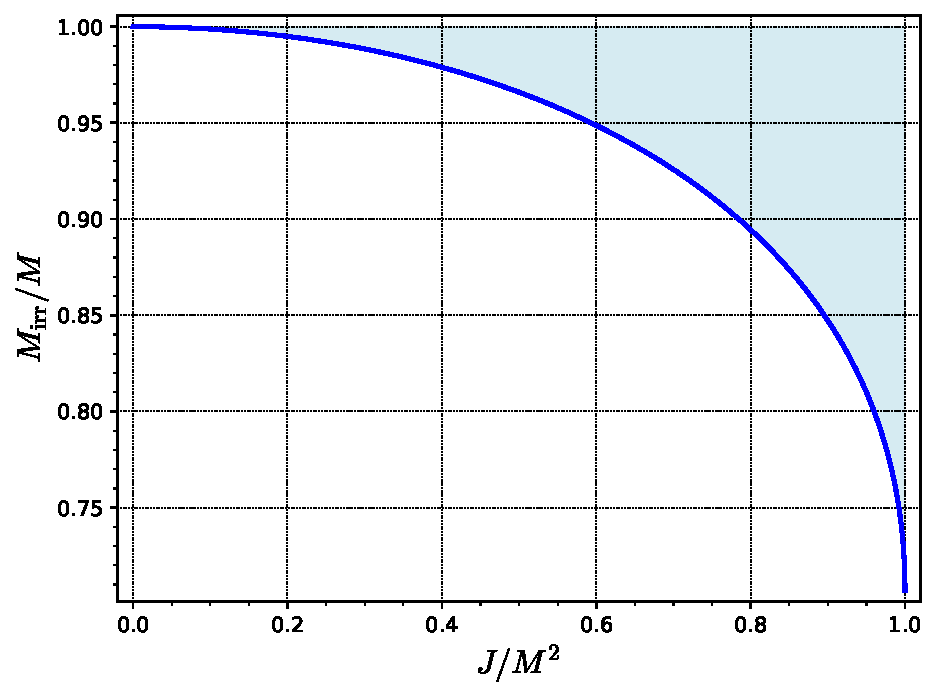
\includegraphics[width=0.6\textwidth]{evo_irred_mass.pdf}}
\caption[]{\label{f:evo:irred_mass} \footnotesize
Irreducible mass $M_{\rm irr}$ of a Kerr black hole of mass $M$, as a
function of the black hole angular momentum $J$ [Eq.~(\ref{e:evo:M_irr_M_J})]
($J = 0$ corresponds to a
Schwarzschild black hole and $J/M^2 = 1$ to an extremal Kerr one). The shadded
area depicts the maximal energy that can be extracted from the black hole by
a Penrose process bringing $J$ down to $0$.}
\end{figure}

Suppose some energy is extracted by a sequence of Penrose processes\index{Penrose!process}
(cf. Sec.~\ref{s:gek:Penrose_proc}) from a Kerr black hole of initial mass $M$ and angular momentum $J$,
leading to a final state corresponding to a Kerr black hole of mass $M_0$ and angular
momentum $J_0$. The maximal energy $\Delta M = M - M_0$ that can be extracted is achieved when the
final state is a Schwarzschild black hole ($J_0=0$), since then the Penrose process
necessarily stops, due to the lack of an outer ergoregion (cf. Sec.~\ref{s:gek:Penrose_proc}).
Since the irreducible mass of a Schwarzschild black hole coincides with its mass
(set $J=0$ in Eq.~(\ref{e:evo:M_irr_M_J})), the irreducible mass
of the final state is $M_{{\rm irr},0} = M_0$ and we have $\Delta M = M - M_{{\rm irr},0}$.
The evolution law $M_{{\rm irr},0} \geq M_{\rm irr}$ provides then a upper bound
on the extracted energy:
\be
    \Delta M \leq M - M_{\rm irr} ,
\ee
with equality only for a sequence of reversible transformations.
Figure~\ref{f:evo:irred_mass} shows that $\Delta M/M$ is maximal when the
initial state is (close to) an extremal Kerr black hole ($J=M^2$). From
Eq.~(\ref{e:evo:M_irr_M_J}), one gets
\be
    \max \frac{\Delta M}{M} = 1 - \frac{1}{\sqrt{2}} \simeq 0.293 .
\ee
We conclude:
\begin{prop}[maximal energy extraction by a Penrose process]
A sequence of Penrose processes can extract up to $29 \%$ of the mass
of a Kerr black hole. This upper bound is achieved for
a maximally spinning black hole (extremal Kerr), by bringing it down to a non-rotating
state (Schwarzschild) via reversible transformations.
\end{prop}

\begin{hist}
\label{h:evo:irreducible_mass}
Demetrios Christodoulou\index[pers]{Christodoulou, D.} introduced the
concepts of \emph{irreversible transformation} and \emph{irreducible mass} of a Kerr black
hole in 1970 \cite{Chris70} and established formula (\ref{e:evo:M_M_irr_J}).
Actually, he did not make any argument about the black hole area; rather he
integrated the relation $\D M = \Omega_{\Hor} \, \D J$, which holds when
the black hole is accreting a particle with $E_* = \Omega_{\Hor} L_*$ (cf. Eq.~(\ref{e:evo:dM_E_dJ_L}), i.e.
at the saturation limit of the inequality (\ref{e:gek:OmegaH_Lpp_Epp}). Indeed, by expressing
$\Omega_{\Hor}$ as a function of $(M,J)$ via Eq.~(\ref{e:ker:def_OmegaH}),
one gets $\D M = J\D J/(2M(M^2 + \sqrt{M^4 - J^2}))$, which is equivalent
to $\D(M^2 + \sqrt{M^4 - J^2}) = 0$.
The irreducible mass $M_{\rm irr}$
then appears when writing the integration constant for this equation as $2 M_{\rm irr}^2$,
namely $M^2 + \sqrt{M^4 - J^2} = 2 M_{\rm irr}^2$, which is equivalent to Eq.~(\ref{e:evo:M_irr_M_J}).
The connection with the black hole area [Eq.~(\ref{e:evo:Mirr_A})] has been
performed in a second study, with Remo Ruffini\index[pers]{Ruffini, R.}, published in 1971
\cite{ChrisR71} and which extends Christodoulou's results to Kerr-Newmann
black holes\index{Kerr-Newman!black hole}. Meanwhile,
Roger Penrose\index[pers]{Penrose, R.}
and Roger Floyd\index[pers]{Floyd, R.M.} noticed at the end of 1970 (published 1971 \cite{PenroF71})
that the area of a Kerr black hole necessarily increases under particle accretion, i.e.
they established Property~\ref{p:evo:area_law_Kerr}.
In 1972, Brandon Carter\index[pers]{Carter, B.} \cite{Carte72} pointed out that the relation
$\D M = \Omega_{\Hor} \, \D J$ also holds for a rigidly rotating fluid star undergoing a
thermodynamically reversible transformation (in that case, $\Omega_{\Hor}$ stands for
the star's angular velocity). This strengthened the analogy between irreversibility in
black hole processes and standard thermodynamics.
\end{hist}

\subsection{Hawking's area theorem}

The area increase law turns out to be far
more general than established in Property~\ref{p:evo:area_law_Kerr},
which regards only a Kerr black hole accreting particles:
the law actually applies to any black hole evolving under
any process (not necessarily a small perturbation) such that the null convergence condition
[Eq.~(\ref{e:neh:null_energy_cond})]
is satisfied in the vicinity of the event horizon.
This is the essence of the famous \emph{area theorem}, first established
by Hawking in 1971.

The first step towards the area theorem is:

\begin{prop}[positive expansion of a black hole horizon\index{expansion!positive -- theorem}]
\label{p:evo:positive_expansion}
Let $(\M,\w{g})$ be a $n$-dimensional spacetime containing a black hole
of event horizon $\Hor$. If the Ricci tensor $\w{R}$ obeys the null
convergence condition\index{null!convergence condition}\index{convergence!condition!null --} (\ref{e:neh:null_energy_cond}) on $\Hor$, i.e. if
$\w{R}(\wl, \wl) \geq 0$ for any null vector $\wl$ on $\Hor$
--- which holds in general relativity if the null energy condition\index{null!energy condition}\index{energy!condition!null --} (\ref{e:neh:null_energy_cond_matter}) is fulfilled ---, then the
expansion $\theta_{(\wl)}$ of $\Hor$ along any future-directed null
normal $\wl$, as defined in Sec.~\ref{s:def:def_expansion}, is positive or zero:
\be \label{e:evo:theta_positive}
    \theta_{(\wl)} \geq 0 .
\ee
\end{prop}
\begin{proof}
Let $\wl$ be a future-directed null normal vector field of $\Hor$.
$\wl$ is necessarily tangent to the null geodesic geodesic generators of $\Hor$
(Property~\ref{p:def:null_geod_generators}) and is thus a pregeodesic
vector, i.e. it obeys Eq.~(\ref{e:def:wl_geod_kappa}):
$\wnab_{\wl}\, \wl = \kappa \, \wl $.
If $\wl$ is not geodesic ($\kappa\neq 0$), it is always possible to rescale it
to $\wl' = \alpha \wl$ with $\alpha > 0$ so that $\wl'$ is a future-directed geodesic vector field:
$\wnab_{\wl'}\, \wl' = 0$ [Eq.~(\ref{e:def:wlp_geod})].
We have then $\theta_{(\wl')} = \alpha \theta_{(\wl)}$ [cf. Eq.~(\ref{e:def:rescale_lambda})],
so that $\theta_{(\wl)} \geq 0 \iff \theta_{(\wl')} \geq 0$.
Accordingly, for proving (\ref{e:evo:theta_positive}), there is no loss of generality in assuming that
$\wl$ is a geodesic vector field.
Let us consider a null geodesic generator $\Li$ of $\Hor$. Up to some additive constant, there is
a unique affine parameter $\lambda$ of $\Li$ associated to $\wl$, i.e.  such that
$\wl = \D\w{x}/\D\lambda$ along $\Li$. The evolution of
$\theta_{(\wl)}$ along $\Li$
is measured by $\D\theta_{(\wl)}/\D\lambda = \wnab_{\el}\,  \theta_{(\wl)}$ and is given by
the null Raychaudhuri equation (\ref{e:def:null_Raychaud_Ricci}).
Owing to $\kappa=0$ (for $\wl$ is assumed to be geodesic), it simplifies to
\[
    \derd{\theta_{(\wl)}}{\lambda}  =
        - \frac{1}{n-2} \, \theta_{(\wl)}^2
        - \underbrace{\sigma_{ab} \sigma^{ab}}_{\geq 0}
        - \underbrace{\w{R}(\wl, \wl)}_{\geq 0} ,
\]
where $\sigma_{ab} \sigma^{ab} \geq 0$ has been established in
Sec.~\ref{s:def:null_convergence_cond} [Eq.~(\ref{e:neh:sigma_square})]
and $\w{R}(\wl, \wl) \geq 0$ holds by virtue of the null
convergence condition on $\Hor$. Hence
\be \label{e:evo:der_theta_lower}
    \derd{\theta_{(\wl)}}{\lambda}  \leq
        - \frac{1}{n-2} \, \theta_{(\wl)}^2  .
\ee
Let us assume the negation of (\ref{e:evo:theta_positive}), i.e. that there
exists a point $p\in\Li\cap\Hor$ where $\theta_{(\wl)} = \theta_0 < 0$.
By choosing the additive constant in the definition of the affine parameter $\lambda$,
we may ensure $\lambda(p) = 0$.
Equation~(\ref{e:evo:der_theta_lower}) implies then
\be \label{e:evo:theta_lower_theta_bar}
 \forall \lambda\geq 0,\quad \theta_{(\wl)}(\lambda) \leq \bar\theta(\lambda) ,
\ee
where $\bar\theta(\lambda)$ obeys
\[
    \frac{\D\bar\theta}{\D\lambda} = -  \frac{1}{n-2}  \bar\theta^2
    \qand \bar\theta(0) = \theta_0 .
\]
The unique solution of this differential equation is
\[
\bar\theta(\lambda) = \frac{\theta_0}{1 + \theta_0\lambda/(n-2)} .
\]
It follows that $\bar\theta \to -\infty$ as $\lambda \to -(n-2)/\theta_0 > 0$.
The inequality~(\ref{e:evo:theta_lower_theta_bar}) then implies
$\theta_{(\wl)} \to -\infty$ as $\lambda \to \lambda_*$
with $0 < \lambda_* \leq -(n-2)/\theta_0$. Hence the point $p_*\in\Li$ of parameter $\lambda_*$ is a \emph{focusing point},
i.e. a point where neighboring null geodesic generators of $\Hor$ intersect.
But according to Property~\ref{p:glo:prop3} of black hole event horizons (cf. Sec.~\ref{s:glo:properties_H}), this can happen
only if $p_*$ is a crossover point, i.e.
a point at which the null geodesic $\Li$ enters $\Hor$; however,
this situation is excluded since $\lambda_* > 0$ implies that $p_*$ lies in the
future of $p$, where $\Li$ is already in $\Hor$. Hence the hypothesis
$\theta_0 < 0$ leads to a contradiction. It follows that $\theta_0 \geq 0$,
i.e. at any point $p\in\Hor$,  $\theta_{(\wl)} \geq 0$.
\end{proof}

\begin{figure}
\centerline{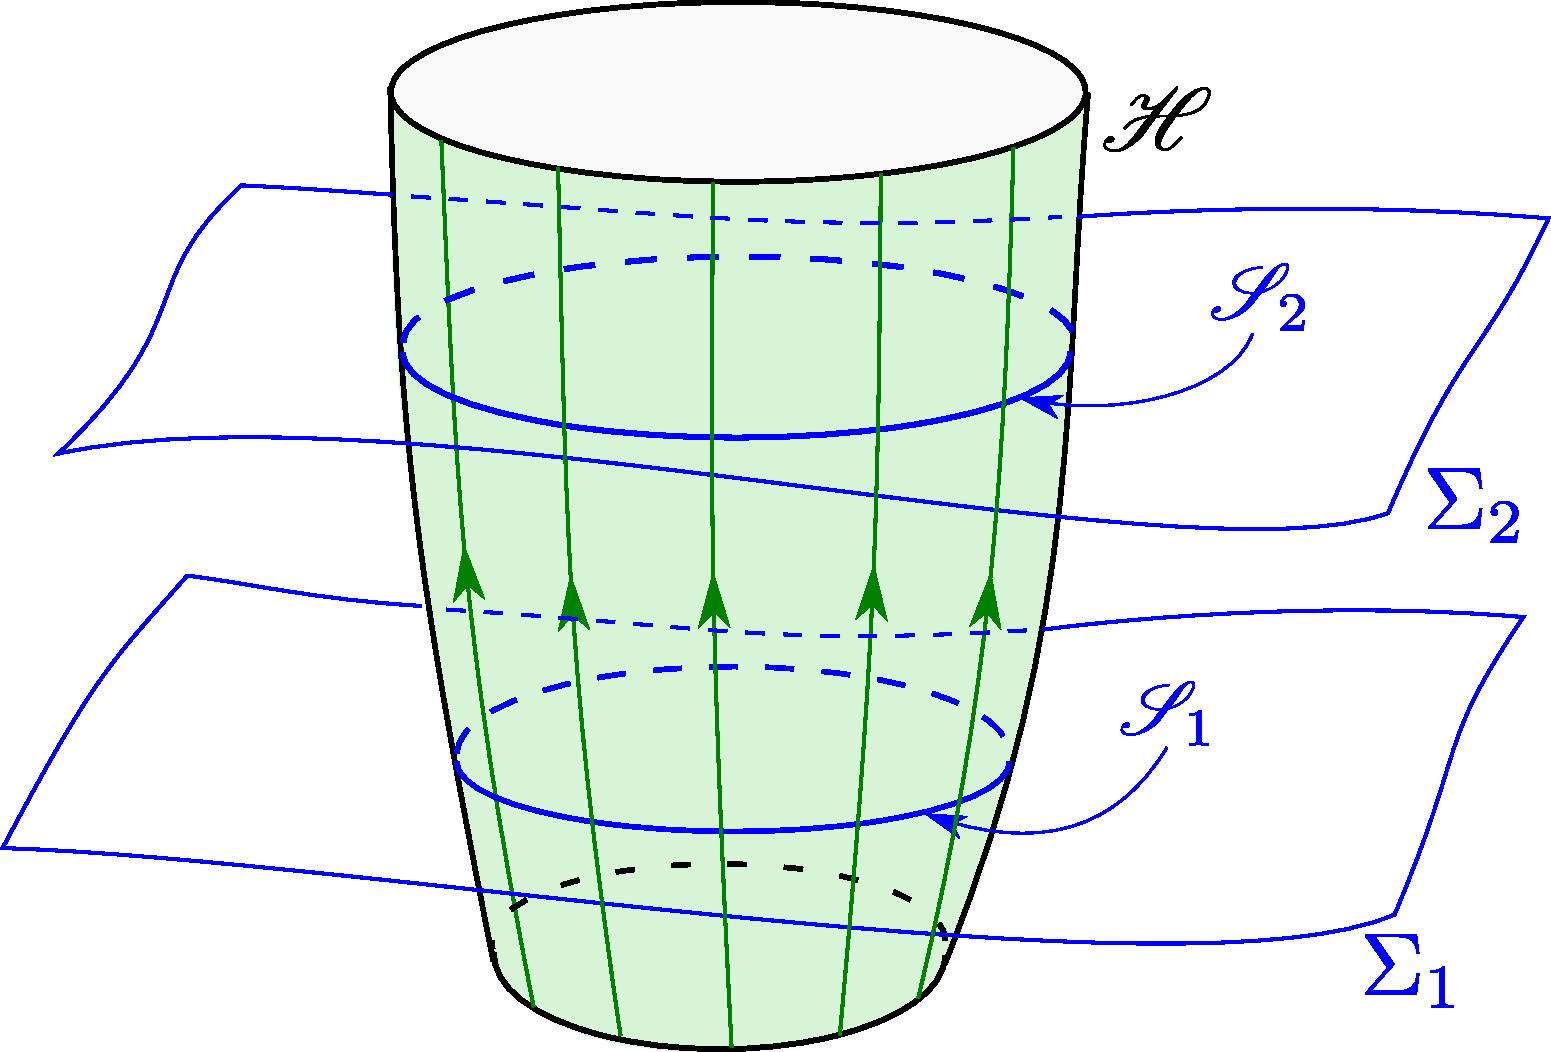
\includegraphics[width=0.6\textwidth]{evo_area_thm_smooth.pdf}}
\caption[]{\label{f:evo:area_thm_smooth} \footnotesize
Cross-sections $\Sp_1$ and $\Sp_2$ induced by the spacelike hypersurfaces $\Sigma_1$
and $\Sigma_2$ in a smooth part of the event horizon $\Hor$,
such that $\Sp_1$ and $\Sp_2$ are intersected by the same null geodesic
generators of $\Hor$ (green curves).}
\end{figure}



\begin{prop}[area theorem\index{area!theorem} \textnormal{(Hawking\index[pers]{Hawking, S.W.} 1971 \cite{Hawki71},
Chru\'sciel\index[pers]{Chrusciel, P.T.@Chru\'sciel, P.T.},
Delay\index[pers]{Delay, E.},
Galloway\index[pers]{Galloway, G.J.} and Howard\index[pers]{Howard, R.} 2001
\cite{ChrusDGH01})}]
\label{p:evo:area_thm}
Let $(\M,\w{g})$ be a spacetime of dimension $n\geq 2$ that contains a black hole
of event horizon $\Hor$. Let us assume that the Ricci tensor $\w{R}$ fulfills the null
convergence condition\index{null!convergence condition}\index{convergence!condition!null --} (\ref{e:neh:null_energy_cond}), i.e.
$\w{R}(\wl, \wl) \geq 0$ for any null vector $\wl$
--- which holds in general relativity if the null energy condition\index{null!energy condition}\index{energy!condition!null --} (\ref{e:neh:null_energy_cond_matter}) is fulfilled.
Let $\Sigma_1$ and $\Sigma_2$ be spacelike hypersurfaces
such that $\Sigma_2$ lies in the causal future of $\Sigma_1$: $\Sigma_2\subset J^+(\Sigma_1)$
(cf. Sec.~\ref{s:glo:causal_struct}). Let $\Sp_1 = \Hor \cap \Sigma_1$
and $\Sp_2 = \Hor\cap\Sigma_2$.
If
\begin{itemize}
\item[(i)] $\Hor$ is smooth between $\Sp_1$ and $\Sp_2$, and $\Sp_1$ and $\Sp_2$
are cross-sections\footnote{If $\Hor$ is smooth between $\Sp_1$ and $\Sp_2$,
it is necessarily a null hypersurface there (Property~\ref{p:glo:prop4} on p.~\pageref{p:glo:prop4}),
so that the concept of cross-section as defined in Sec.~\ref{s:def:spacelike_sections}
makes sense.} of $\Hor$ that are intersected by the same null geodesic generators of $\Hor$
(cf. Fig.~\ref{f:evo:area_thm_smooth})
\end{itemize}
or
\begin{itemize}
\item[(ii)]
the closure of $J^-(\scri^+)\cup \Hor$ in
the conformal manifold $\tilde{\M}\supset\M$ defining $\scri^+$
is included in a globally hyperbolic
region $\mathscr{V}$ of $(\tilde{\M},\tilde{\w{g}})$
and $\Sigma_1$ and $\Sigma_2$ are Cauchy surfaces
of $\mathscr{V}$,
\end{itemize}
then the areas $A(\Sp_1)$ and $A(\Sp_2)$ obey
\be \label{e:evo:AS2_ge_AS1}
    A(\Sp_2) \geq A(\Sp_1) .
\ee
\end{prop}

\begin{figure}
\centerline{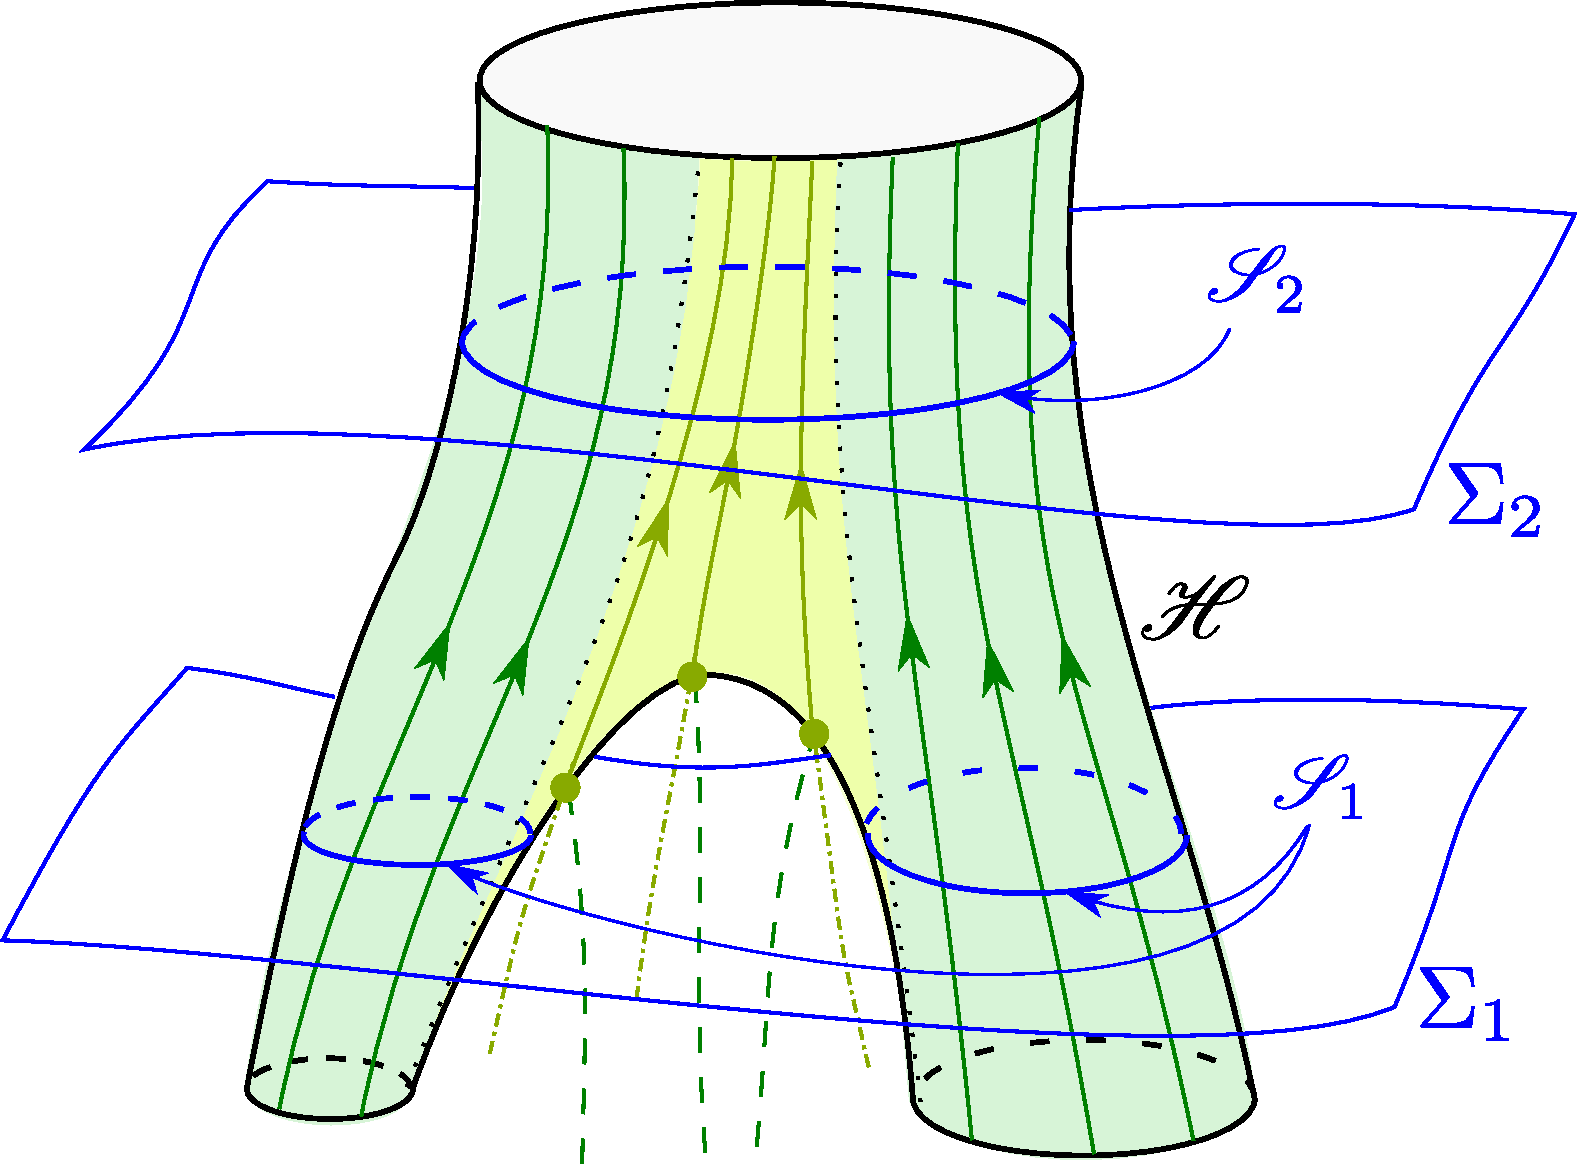
\includegraphics[width=0.6\textwidth]{evo_area_theorem.pdf}}
\caption[]{\label{f:evo:area_theorem} \footnotesize
Surfaces $\Sp_1$ and $\Sp_2$ induced by the spacelike hypersurfaces $\Sigma_1$
and $\Sigma_2$ on the event horizon $\Hor$ corresponding to a black hole merger.
All solid dark green and light green curves are null geodesic generators of $\Hor$.
The light green part of $\Hor$ is generated by null geodesics that
entered $\Hor$ at some caustic points (three of them are indicated as
light green dots); the parts of these geodesics outside $\Hor$ are drawn as
light green dot-dashed curves. The dark green dashed curves depict other null geodesics that
enter $\Hor$ at the same caustic points.}
\end{figure}


\begin{proof}
For $n=2$, the theorem is trivial since $\Sp_1$ and $\Sp_2$ are reduced to
points, so that $A(\Sp_1) = A(\Sp_2) = 0$ and Eq.~(\ref{e:evo:AS2_ge_AS1}) is fulfilled.
Let us then assume $n\geq 3$.
We consider first the case (i) ($\Hor$ smooth between
$\Sp_1$ and $\Sp_2$).
$\Sp_1$ and $\Sp_2$ are then cross-sections of $\Hor$
that are connected by null geodesic generators of $\Hor$
(cf. Fig.~\ref{f:evo:area_thm_smooth}).
One may introduce a 1-parameter foliation $(S_t)_{t\in [0,1]}$ of $\Hor$ by
cross-sections $S_t$ such that $S_0 = \Sp_1$ and $S_1 = \Sp_2$
(cf. the proof of Property~\ref{p:neh:invariance_area} for details, $\lambda$
playing the role of $t$ there). The label $t$
can then be considered as a parameter along the null geodesic generators of $\Hor$
connecting $\Sp_1$ to $\Sp_2$.
Let $\wl = \D\w{x}/\D t$ be the associated tangent vector.
Given that $\Sp_2$ lies in the future of $\Sp_1$, $\wl$ is future-directed.
By the very definition
of the expansion $\theta_{(\wl)}$ along $\wl$ [Eq.~(\ref{e:def:def_expansion})
combined with Eq.~(\ref{e:def:A_sqrt_q})], one has
\[
    \derd{}{t} A(S_t) = \int_{S_t} \theta_{(\wl)} \,  \sqrt{q} \, \D x^2 \cdots \D x^{n-1} ,
\]
where $(x^2, \ldots, x^{n-1})$ is a coordinate system on $S_t$ and $q$ is
the determinant with respect to these coordinates of the metric
induced by $\w{g}$ on $S_t$.
Now, if the null convergence condition holds, Property~\ref{p:evo:positive_expansion} implies
$\theta_{(\wl)} \geq 0$; hence
\[
  \derd{}{t} A(S_t) \geq 0 .
\]
It follows that $t\mapsto A(S_t)$ is a nondecreasing function. Consequently, $A(S_1) \geq A(S_0)$
and Eq.~(\ref{e:evo:AS2_ge_AS1}) holds.

If $\Hor$ is not smooth between $\Sp_1$ and $\Sp_2$, this is due to the crease set\index{crease set},
i.e. the subset of $\Hor$ where new null geodesics enter $\Hor$ (cf. Sec.~\ref{s:glo:properties_H}).
Naively, this reinforces the inequality $A(\Sp_2) > A(\Sp_1)$ since the new geodesics
are generating new parts of $\Hor$ and therefore parts of $\Sp_2$ distinct
from those that can be connected to $\Sp_1$ by null geodesic generators
(cf. Fig.~\ref{f:evo:area_theorem}). More precisely, let us assume (ii) and
let us consider a point $p\in\Sp_1$. Let $\Li$ be the null geodesic
generator of $\Hor$ through $p$. By property~\ref{p:glo:prop3}, $\Li$ stays in $\Hor$ for all its future after $p$. Since $\Sigma_2$ is a Cauchy surface lying in the causal future of $\Sigma_1$, $\Li$
necessarily intersects $\Sigma_2$ at a unique point $q \in \Sigma_2\cap\Hor = \Sp_2$.
Hence every point of $\Sp_1$ is mapped to a point of $\Sp_2$ by a null geodesic generator.
Let $\Sp_2^*$ be the part of $\Sp_2$ covered by this map.
If we assume that the part of $\Hor$ between $\Sp_1$ and $\Sp_2^*$ is smooth,
we may apply (i) to the pair $(\Sp_1, \Sp_2^*)$
and get $A(\Sp_2^*) \geq A(\Sp_1)$. Given that $\Sp_2^* \subset \Sp_2$, one has
$A(\Sp_2) \geq A(\Sp_2^*)$ and (\ref{e:evo:AS2_ge_AS1}) follows.
We refer to the article \cite{ChrusDGH01} for the proof in the case where
$\Hor$ is not assumed smooth between $\Sp_1$ and $\Sp_2^*$ (70 pages!).
\end{proof}

\begin{example}[Oppenheimer-Snyder collapse]
Let us consider the black hole formed by the collapse
of a ball of pressureless matter, as described by the Oppenheimer-Snyder
model studied in Sec.~\ref{s:lem:OS}. Let $\Sp_{\ti}$ be a
cross-section of the event horizon at constant ingoing Eddington-Finkelstein coordinate $\ti$.
The area of $\Sp_{\ti}$ is simply $A = 4\pi r^2$,
where $r$ is the areal radius (cf. Sec.~\ref{s:lem:OS:BH_formation}). Its
evolution can thus be read directly on Fig.~\ref{f:lem:OS:diag_int_EF} (right):
it is increasing from $A = 0$ (at $\ti\simeq 5.6\, m$) to the Schwarzschild
value $A = 16\pi m^2$ (at $\ti\simeq 9.7\, m$). This fully agrees
with the area theorem, given that the null energy condition (\ref{e:neh:null_energy_cond_matter})
is fulfilled by the energy-momentum tensor (\ref{e:lem:T_pressureless}) of the collapsing matter: $\w{T}(\wl,\wl) =  \rho (\w{u}\cdot\wl)^2 \geq 0$ since $\rho \geq 0$.
\end{example}

\begin{example}[Vaidya collapse]
Similarly, we check on Figs.~\ref{f:vai:diag_S0} and \ref{f:vai:diag_S2}
that for the radiation shell collapse studied in Chap.~\ref{s:vai},
the area of cross-sections of the event horizon
at constant ingoing Eddington-Finkelstein coordinate $t$
is increasing towards the future, for $r$ is again the areal radius
[cf. the metric (\ref{e:vai:metric_IEF})]. As we have already noticed in
Sec.~\ref{s:vai:general}, the radiation energy-momentum tensor (\ref{e:vai:ener_mom_tensor})
fulfills the null energy condition, given that $M'(v) \geq 0$ (cf. Fig.~\ref{f:vai:mass_function}).
\end{example}


\begin{hist} \label{h:evo:area_increase}
As mentioned in the historical note on p.~\pageref{h:evo:irreducible_mass},
Roger Penrose\index[pers]{Penrose, R.}
and Roger Floyd\index[pers]{Floyd, R.M.} \cite{PenroF71}
have shown in 1970 (published 1971)
that the area of a Kerr black hole always increases during particle accretion,
even if its mass is decreasing, as in a Penrose process (Property~\ref{p:evo:area_law_Kerr}).
Soon after, in 1971, Stephen Hawking\index[pers]{Hawking, S.W.}
\cite{Hawki71} established the area theorem for generic
dynamical black holes and a detailed proof was given in
Hawking \& Ellis' 1973 textbook (Proposition~9.2.7 in \cite{HawkiE73}).
In 2001, Piotr Chru\'sciel\index[pers]{Chrusciel, P.T.@Chru\'sciel, P.T.},
Erwann Delay\index[pers]{Delay, E.},
Gregory Galloway\index[pers]{Galloway, G.J.} and Ralph Howard\index[pers]{Howard, R.}
\cite{ChrusDGH01} pointed out that the Hawking \& Ellis proof is
valid only for $\Hor$ piecewise smooth (cf. the
discussion in Sec.~3.5.1 of Chru\'sciel's textbook \cite{Chrus20}); they constructed
a new proof that does not rely on the smoothness of $\Hor$.
\end{hist}

\subsection{A second law?}

Basically the area theorem~\ref{p:evo:area_thm} states that
the area of cross-sections of a black hole event horizon
cannot decrease from the past to the future.
By its irreversible character, this property bears some resemblance
with the second law of thermodynamics.
By itself, this is of course not sufficient to identify the black hole area
with some entropy (any nondecaying physical quantity has not to be an entropy!).
However, we have seen in Sec.~\ref{s:evo:a_first_law_question} that the
candidate $T\D S$ term for a possible first law could be $\kappa/(8\pi)\D A$.
It is thus tempting to identify $A$ with an entropy $S$, up to some
constant factor $\alpha$. Then the temperature $T$ would be $\kappa/(8\pi\alpha)$:
\begin{subequations}
\label{e:evo:identif_S_T}
\begin{align}
  S & = \alpha A \label{e:evo:identif_S_A}\\
  T &= \frac{1}{8 \pi\alpha}\, \kappa , \label{e:evo:identif_T_kappa}
\end{align}
\end{subequations}
so that $\kappa/(8\pi)\D A = T\D S$, which makes
the mass variation formula (\ref{e:evo:mass_variation_vacuum_n4}) look pretty much like
the first law of thermodynamics.

%%%%%%%%%%%%%%%%%%%%%%%%%%%%%%%%%%%%%%%%%%%%%%%%%%%%%%%%%%%%%%%%%%%%%%%%%%%%%%%

\section{The laws of black hole dynamics}

In Secs.~\ref{s:evo:towards_1st_law} and \ref{s:evo:evol_area}, we have established black hole
properties that are quite analog to the first and second laws of thermodynamics. Let us now
examine the zeroth and third laws of thermodynamics.

\subsection{Zeroth law}

We have already established a so-called \emph{zeroth law of black hole dynamics}
in Chap.~\ref{s:neh}, namely the surface gravity
$\kappa$ of a Killing horizon is constant, provided that the
null dominance condition is fulfilled (Property~\ref{p:neh:zeroth_law})
or that the Killing horizon is part of a bifurcate Killing horizon
(Property~\ref{p:neh:zeroth_law_bifur}).
Now, by Properties~\ref{p:sta:H_Killing_hor_xi_null}
and \ref{p:sta:strong_rigidity_thm}, (a connected component of) the event horizon
of a stationary black hole must be a Killing horizon. Hence, we may extend
the zeroth law to black holes\index{zeroth law!of BH dynamics}:

\begin{prop}[zeroth law of black hole dynamics]
\label{p:evo:zeroth_law}
Let $(\M,\w{g})$ be a stationary spacetime of dimension $n\geq 4$
containing a black hole.
Let $\Hor$ be a connected component of the black hole event horizon.
If $\Hor$ is non-rotating (i.e. if the stationary Killing vector $\w{\xi}$ is null
on $\Hor$), $\Hor$ is necessarily a Killing horizon (Property~\ref{p:sta:H_Killing_hor_xi_null}).
If $\Hor$ is rotating
($\w{\xi}$ spacelike on some parts of $\Hor$),
we shall assume that the hypotheses of the strong rigidity theorem
(Property~\ref{p:sta:strong_rigidity_thm}) hold, so that $\Hor$ is a Killing horizon as well.
If the null dominance condition\index{null!dominance condition}\index{dominance!null -- condition} (\ref{e:neh:null_dominant_cond})
is fulfilled on $\Hor$  --- which is guaranteed in general relativity
if the null dominant energy condition\index{null!dominant energy condition}\index{energy!condition!null dominant --} (\ref{e:neh:null_dominant_cond_T}) holds on $\Hor$ ---
or if $\Hor$ is part of a bifurcate Killing horizon,
then the surface gravity $\kappa$ is constant over $\Hor$.
\end{prop}

Given that a black hole ``in equilibrium'' is modeled by a black hole in
a stationary spacetime,
this property bears a strong resemblance with
the \emph{zeroth law of thermodynamics}\index{zeroth law!of thermodynamics}, which states that the temperature of a body in equilibrium
is uniform over the entire body.
This strengthens the interpretation of the surface gravity
$\kappa$ as the temperature $T$ (up to some factor) performed in
Eq.~(\ref{e:evo:identif_T_kappa}).


\subsection{What about the third law?} \label{s:evo:third_law}

The classical Nernst formulation of the \emph{third law of thermodynamics}\index{third law!of thermodynamics}
states that the entropy of a system must approach zero (or a universal constant)
as its temperature tends to zero. In this form and with the identification (\ref{e:evo:identif_S_T}), this law certainly does not hold for black holes, because
extremal\index{extremal!black hole} black holes, which have $\kappa=0$, have a non-vanishing area. For
instance, the area of the extremal Kerr black hole\index{extremal!Kerr!spacetime}\index{Kerr!extremal -- spacetime} of mass $m$ (Chap.~\ref{s:exk}) is
$A = 8\pi m^2$ (take the limit $a\to m$ in Eq.~(\ref{e:ker:A_a_m})),
which is neither zero, nor a universal constant. Similarly, the area of
the extremal Reissner-Nordström black hole\index{Reissner-Nordström!black hole!extremal --}\index{extremal!Reissner-Nordström!black hole} of mass $m$ is $A = 4\pi m^2$
(this is immediate from the metric (\ref{e:loc:metric_ERN}) below).
Another formulation of the third law of thermodynamics states that it is impossible to bring any
system to zero temperature by a finite number of operations. This was the formulation adopted
for black holes, as a conjecture, in 1973 by Carter\index[pers]{Carter, B.} \cite{Carte73b} and Bardeen\index[pers]{Bardeen, J.M.}, Carter and Hawking\index[pers]{Hawking, S.W.} \cite{BardeCH73}.
It was then reformulated, with a tentative proof, by Israel\index[pers]{Israel, W.} in 1986 \cite{Israe86b}, as
\begin{quote}
No continuous process in which the energy-momentum tensor of accreted matter remains
bounded and satisfies the weak energy
condition\index{weak!energy condition}\index{energy!condition!weak --} in a neighborhood of the apparent
horizon can reduce the surface gravity of a black hole to zero
within a finite advanced time.
\end{quote}
However, as pointed out recently by Kehle\index[pers]{Kehle, C.} and Unger\index[pers]{Unger, R.} \cite{KehleU23}, Israel's proof
is restricted to the case where outermost trapped surfaces evolve smoothly, while, as we shall discuss in Chap.~\ref{s:loc},
their evolution generically presents discontinuous jumps, even if the spacetime
and all the matter fields remain perfectly smooth. In particular, Kehle and Unger \cite{KehleU23} have exhibited a regular spacetime where the collapse of a charged scalar field (obeying the dominant, and hence the weak, energy condition) turns a Schwarzschild black hole
into an extremal Reissner-Nordström black hole within a finite advanced time\footnote{As shown
in Sec.~5.5.6 of Poisson's textbook \cite{Poiss04}, this cannot happen with a charged null dust
(i.e. a charged generalization of Vaidya collapse discussed in Chap.~\ref{s:vai}) that obeys
the weak energy condition.}.

From an astrophysical point of view, Bardeen\index[pers]{Bardeen, J.M.} has shown in 1970 \cite{Barde70a}
that a Schwarzschild black hole
of mass $m_0$, and hence of surface gravity $\kappa = 1/(4m_0) > 0$ [Eq.~(\ref{e:def:kappa_Schw_hor})],
can in principle be spun up to an extremal\index{extremal!Kerr!spacetime} Kerr black hole
($\kappa = 0$)
by accreting matter from an accretion disk\index{accretion!disk}
terminating at the innermost stable circular orbit\index{innermost!stable circular orbit}\index{circular!orbit!innermost stable --} (ISCO, cf. Sec.~\ref{s:gek:circ_orb_stab}). The total rest-mass of accreted matter is then
$1.86\, m_0$ and the mass of the final black hole is $m \simeq 2.45\, m_0$.
However, if one takes into account the electromagnetic emission of the accretion disk, the extremal Kerr state
cannot be achieved. The reason is that a substantial part of the emitted photons carry a negative angular momentum $\ell$ and
the black hole absorption cross-section for photons with $\ell<0$ is larger than for those with
$\ell>0$. This clearly appears on the shadow picture of Fig.~\ref{f:gik:shadow_a95},
where the part $\alpha>0$, which is due to photons
with $\ell < 0$ (cf. Eq.~\ref{e:gik:shadow_param_eq_alpha}), is much larger than the part $\alpha<0$
corresponding to $\ell > 0$. Consequently, the black hole absorbs more photons with $\ell < 0$
than with $\ell>0$; this diminishes the increase of the black hole spin $a$ induced by accretion of  matter from the disk (which has a positive angular momentum). Thorne\index[pers]{Thorne, K.S.} has shown in 1974 \cite{Thorn74} that the balance between the two processes leads to a final spin parameter $a \simeq 0.998 \, m$, quite insensitive to the details
of the emission mechanism in the accretion disk. This is close to, but strictly lower than, the critical
value $a = m$ that would have yield a zero surface gravity. Hence, in this respect, we may say that
astrophysical black holes absorbing matter from an accretion disk obey a kind of third law.
But this does not appear to arise from some fundamental properties of black holes; it rather results from the properties of their environment.

It must be stressed that in standard thermodynamics as well, the third law has not the same fundamental status as the other laws.
In particular it can be violated by some rather simple systems (see Ref.~\cite{Wald97} for a discussion and an example involving a boson (or fermion) gas confined to a circular ring).

For all the above reasons, we shall no longer discuss the third law here.


\subsection{Summary: the three laws}

Let us collect the results obtained so far, in the form of three laws
similar to the laws of thermodynamics. To stress the analogy, we are using the phrase
\emph{black hole in equilibrium}\index{black!hole!in equilibrium} for \emph{black hole in a stationary spacetime} (cf. Chap.~\ref{s:sta}). Besides, for the sake of brevity, we shall not repeat
the various assumptions underlying these laws, referring to previously
stated properties for all the details. Furthermore, we consider
a connected event horizon for simplicity.

\begin{prop}[laws of black hole dynamics]
\label{p:evo:laws_BH_dyn}
\begin{description}
\item[Zeroth law:]\index{zeroth law!of BH dynamics} Under the hypotheses of Property~\ref{p:evo:zeroth_law},
the surface gravity $\kappa$ of the event horizon of a black hole in equilibrium is
uniform over the horizon:
\be \label{e:evo:zeroth_law}
    \kappa = \mathrm{const}.
\ee
\item[First law:]\index{first law!of BH dynamics} Under the hypotheses of Property~\ref{p:evo:mass_var_electrovac} (in particular, general relativity),
the change $\delta M$ in total mass  between two nearby electrovacuum configurations of
a black hole in equilibrium is related to the change $\delta A$ in horizon area,
the change $\delta J$ in total angular momentum and the change
$\delta Q_{\Hor}$ in electric charge
by\footnote{For simplicity, we are considering
black holes with a connected horizon and a single angular momentum; see
Eq.~(\ref{e:evo:mass_variation_electovac}) for the general formula, where $M$ is denoted by
$M_\infty$ and $J$ by $J_\infty$.}
\be \label{e:evo:first_law}
\delta M = \frac{\kappa}{8\pi} \, \delta A + \Omega_{\Hor} \, \delta J
    + \Phi_{\Hor} \, \delta Q_{\Hor} ,
\ee
where $\Omega_{\Hor}$ and $\Phi_{\Hor}$ are the horizon's angular velocity and
electric potential respectively.
\item[Second law:]\index{second law!of BH dynamics} Under the hypotheses of Property~\ref{p:evo:area_thm},
the area of cross-sections of a black hole event horizon cannot decrease in time:
\be
    A(\Sp_2) \geq A(\Sp_1) ,
\ee
as soon as the cross-section $\Sp_2$ lies in the causal future of the
cross-section $\Sp_1$.
\end{description}
\end{prop}

\begin{remark}
The three laws are valid for any spacetime dimension $n\geq 4$, and even
$n\geq 2$ for the second law. If one assumes that the event horizon is a Killing
horizon, then the zeroth law is valid for $n\geq 2$ as well.
\end{remark}

\begin{hist}
The above ensemble of laws, plus a tentative third law, has been first stated in 1973 by
James Bardeen\index[pers]{Bardeen, J.M.}, Brandon Carter\index[pers]{Carter, B.}
and Stephen Hawking\index[pers]{Hawking, S.W.} in a seminal article
entitled \emph{The Four Laws of Black Hole Mechanics} \cite{BardeCH73}. This
article, which was mostly written during the famous 1972 Les Houches Summer School \cite{DeWit73}, exhibits proofs of the zeroth and first laws for $n=4$,
relies on Hawking's article \cite{Hawki72} for the second law, and presents
the third law as a conjecture, saying that \emph{``there are strong reasons for believing in it''}
(cf. Sec.~\ref{s:evo:third_law}).
\end{hist}

%%%%%%%%%%%%%%%%%%%%%%%%%%%%%%%%%%%%%%%%%%%%%%%%%%%%%%%%%%%%%%%%%%%%%%%%%%%%%%%

\section{Black hole thermodynamics}

In Property~\ref{p:evo:laws_BH_dyn}, we have listed the three laws as those of black hole \emph{dynamics} and not \emph{thermodynamics}, because this still appears as a mathematical analogy without any definite physical content. In particular, if we stick to a
pure classical (i.e. non-quantum) point of view and would like to attribute some
thermodynamic temperature $T$ to a black hole, it should be $T=0$. Indeed, if the black hole is placed in contact with a thermal reservoir of temperature $T_0>0$, energy will necessarily flow from the reservoir to the black hole and not in the reverse way; this implies $T<T_0$, whatever $T_0$.
For a stationary non-extremal black hole ($\kappa\neq 0$), $T=0$ contradicts the tentative identification (\ref{e:evo:identif_T_kappa}) between $T$ and $\kappa$.
It is striking that quantum field theory in curved spacetime
restores the identification, thereby opening the path to a genuine thermodynamics of
black holes. The identification $T\propto \kappa$ arises from Hawking radiation,
which we examine first.

\subsection{Hawking radiation} \label{s:evo:Hawking_rad}

\begin{prop}[Hawking radiation]
Let $(\M,\w{g})$ be a $n$-dimensional ($n\geq 2$) asymptotically flat
spacetime that is stationary and contains a black hole, the event horizon
of which is a Killing horizon of constant surface gravity $\kappa$.
Then, quantum field theory in the curved background $(\M,\w{g})$
predicts that any quantum field gives birth to a thermal radiation
from the black hole to infinity, called
\defin{Hawking radiation}\index{Hawking!radiation}. The radiation temperature
as measured by asymptotic inertial observers at rest with respect to the black hole
is
\be \label{e:evo:Hawking_temp}
    \encadre{T_{\rm H} = \frac{\hbar}{k_{\rm B}} \frac{\kappa}{2\pi} } ,
\ee
where $\hbar = 1.054571817\; 10^{-34} {\rm\; J\, s}$ is the reduced Planck constant and
$k_{\rm B} = 1.380649\; 10^{-23}$ ${\rm\;  J\, K}^{-1}$ is the Boltzmann constant. $T_{\rm H}$ is called the
\defin{Hawking temperature}\index{Hawking!temperature} of the black hole.
\end{prop}

We shall not establish this property here; this is done in many textbooks,
e.g. \cite{Wald84,Wald94,FroloN98,Carro04,FabbrN05}, as well in some review
articles, e.g. \cite{BroutMPS95,Damou04,Jacob96}. Rather, we shall limit
ourselves to a few remarks:


\begin{remark}
Hawking radiation is an outcome of quantum field theory within a fixed \emph{classical} curved background
(see e.g. \cite{Wald94}). It has not been derived from any quantum theory of gravity, i.e. the background spacetime $(\M,\w{g})$ is not quantized. One says that Hawking radiation is
a \emph{semiclassical effect}\index{semiclassical effect}.
\end{remark}

\begin{remark} \label{r:evo:Hawking_rad_kinematic}
The phenomenon of Hawking radiation is essentially kinematic and does not depend on any field equation for the
metric $\w{g}$. In particular it does not rely on the Einstein equation.
Moreover, the Hawking temperature (\ref{e:evo:Hawking_temp}) is independent from the spacetime dimension
$n$ (see e.g. Ref.~\cite{KantiW15} for a detailed discussion).
\end{remark}

\begin{remark}\label{r:evo:Hawking_temp_units}
Formula~(\ref{e:evo:Hawking_temp}) is given for $c=1$
units, which are used throughout the text. If one restores $c$ and considers
that $\kappa$ has the dimension of an acceleration, the formula should read
$T_{\rm H} = \frac{\hbar}{k_{\rm B}} \frac{\kappa}{2\pi c}$.
\end{remark}

\begin{remark}\label{r:evo:local_Hawking_rad}
The Hawking temperature $T_{\rm H}$ is the radiation temperature measured
infinitely far from the black hole; it is not a ``local'' temperature
measured in the vicinity of the event horizon $\Hor$.
More precisely, let us assume for simplicity that the black hole is non-rotating
(cf. Property~\ref{p:sta:xi_tangent_H}) and that its exterior is strictly static.
The stationary Killing vector $\w{\xi}$ is then null on $\Hor$  and
timelike in the black hole exterior. Let us consider static observers at a finite distance
from $\Hor$, i.e. observers
of 4-velocity $\w{u} = \w{\xi} / V$, where $V := \sqrt{-\w{\xi}\cdot\w{\xi}}$
[cf. Eqs.~(\ref{e:neh:def_u_stationary_obs}) and (\ref{e:neh:def_V_norm_xi})].
The temperature of the Hawking radiation measured by these observers is
\footnote{Cf. e.g. Eq.~(7.2.10) in \cite{Wald94}; in view of Eq.~(\ref{e:evo:Hawking_temp_local}), we may say
that Hawking radiation obeys \defin{Tolman-Ehrenfest law}\index{Tolman-Ehrenfest law}, which
states that the temperature $T$ of a medium in thermal equilibrium in a stationary gravitational field
obeys $T V = \mathrm{const}$ \cite{SantiV19}.}
\be \label{e:evo:Hawking_temp_local}
    T = \frac{T_{\rm H}}{V} .
\ee
For infinitely distant observers, $V\to 1$ [cf. Eq.~(\ref{e:sta:xi_scri})], and we recover $T=T_{\rm H}$.
For static observers infinitely close to the event horizon, $V\to 0$ and we get
$T\to +\infty$. Note that those observers are
also experiencing an infinite acceleration [cf. Eq.~(\ref{e:neh_diverging_accel})].
On the contrary, a freely-falling observer crossing the horizon measures
$T=0$, i.e. she does not detect the Hawking radiation (cf. Remark~\ref{r:evo:Unruh_effect} hereafter).
\end{remark}

\begin{remark} \label{r:evo:Unruh_effect}
The Hawking radiation is closely related to the
\defin{Unruh effect}\index{Unruh effect}, which is another prediction of quantum field theory:
in vacuum Minkowski spacetime, a uniformly accelerated observer measures a black-body radiation
of all particle species at the temperature $T_{\rm U} = (\hbar/k_{\rm B}) \, a / (2\pi)$, where
$a = \sqrt{\w{a}\cdot\w{a}}$ is the norm of the observer's 4-acceleration \cite{Unruh76,Wald94,Carro04}.
A static observer $\Obs$ close to the black hole horizon $\Hor$, as considered in Remark~\ref{r:evo:local_Hawking_rad},
feels an acceleration given by Eq.~(\ref{e:neh:kappa_lim_Va}): $a \sim \kappa / V$.
By combining formulas~(\ref{e:evo:Hawking_temp_local}) and (\ref{e:evo:Hawking_temp}),
we may then rewrite the radiation temperature $T$ measured by $\Obs$ as
$T \sim (\hbar/k_{\rm B}) \, a / (2\pi)$. Hence, it coincides with the Unruh temperature $T_{\rm U}$ of
the observer in Minkowski spacetime sharing the same acceleration $a$ as $\Obs$.
This is somehow expected
if one assumes that freely-falling observers near $\Hor$ perceive quantum states identical to
the Minkowski vacuum (no radiation).
\end{remark}

\begin{remark} \label{r:evo:comp_Hawking_rad}
In terms of elementary particles, the Hawking radiation is composed of
all existing species of massless and massive particles. For the latter ones,
the contribution is significant only if
$k_{\rm B} T_{\rm H} > m_{\rm p}$, where $m_{\rm p}$ is the particle's mass.
For Schwarzschild black holes of mass $M \gg 2\; 10^{13} {\rm\; kg}$ (the threshold
for $k_{\rm B} T_{\rm H}$ being lower than the electron mass, see below), the Hawking radiation
is composed quasi-exclusively of neutrinos ($87\%$ of the radiated energy),
photons ($12\%$) and possibly gravitons ($1\%$) \cite{Page76,ThornZP86}.
\end{remark}

\begin{remark}
The observed radiation spectrum at infinity is not exactly that
of a black body\index{black!body} of temperature $T_{\rm H}$: it is corrected
by greybody factors, which originate from the interaction of the radiation
with the spacetime curvature (backscattering).
\end{remark}

For a Kerr black hole, the surface gravity $\kappa$ is given by formula (\ref{e:ker:kappa_m_a}),
so that the Hawking temperature can be expressed in terms
of the black hole mass $M=m$ and the dimensionless spin parameter
$\bar{a} := a/m = J/M^2$ ($0\leq \bar{a}\leq 1$):
\be \label{e:evo:T_H_Kerr}
   \encadre{ T_{\rm H} = \frac{\hbar}{k_{\rm B}} \frac{c^3}{8\pi G M}
   \; \frac{2}{1 + (1 - \bar{a}^2)^{-1/2}} } _{\rm\; Kerr}.
\ee
Note that we have restored the gravitational constant $G$ and the speed of light $c$
(cf. Remark~\ref{r:evo:Hawking_temp_units}). Numerically, we get
\be
    T_{\rm H} = 6.17\; 10^{-8} \left( \frac{M_\odot}{M} \right)
    \frac{2}{1 + (1 - \bar{a}^2)^{-1/2}} {\rm\; K},
\ee
or, in units more adapted to small black holes,
\be
    k_{\rm B} T_{\rm H}= 1.057\; 10^{10} \left( \frac{1 {\rm\; kg}}{M} \right)
    \frac{2}{1 + (1 - \bar{a}^2)^{-1/2}} {\rm\; GeV}.
\ee
Hence, for a Schwarzschild black hole ($\bar{a}=0$),
$T_{\rm H} = 6.17\; 10^{-8} ({M_\odot}/{M}) {\rm\; K}$. For astrophysical black holes,
this leads to tiny temperatures: $T_{\rm H} \simeq 4\; 10^{-9} {\rm\; K}$
for a $15 \, M_\odot$ stellar black hole (e.g. Cyg X-1, cf. Table~\ref{t:ges:time_free_fall}),
$T_{\rm H} \simeq 1.6\; 10^{-14} {\rm\; K}$ for the Milky Way central black hole Sgr~A*
($M=4.1\; 10^{6} \, M_\odot$)
and $T_{\rm H} \simeq 9\; 10^{-18} {\rm\; K}$ for M87*
($M=6.5\; 10^{9} \, M_\odot$). The value $T_{\rm H} = 1 {\rm\; K}$ is achieved
for a black hole of mass $6.17\; 10^{-8} \, M_\odot$, i.e. $2\, \%$ of the
Earth's mass, while the value $k_{\rm B} T_{\rm H} = m_{\rm e} c^2$
($m_{\rm e} = 9.11\; 10^{-31}\; {\rm kg}$ being the electron mass) is achieved
for $M = 2.07\; 10^{13}\; {\rm kg}$.

Another conclusion that one can draw from formula (\ref{e:evo:T_H_Kerr}) is
that $T_{\rm H}=0$ for an extremal Kerr black hole\index{extremal!Kerr!spacetime}\index{Kerr!extremal -- spacetime} ($\bar{a}=1$): such an object does not emit any Hawking radiation.

\begin{remark} \label{r:evo:negative_heat_capacity}
Formula~(\ref{e:evo:T_H_Kerr}) shows that a Schwarzschild black hole ($\bar{a} = 0$)
has a \emph{negative heat capacity}\index{heat capacity}:
its temperature increases while its energy
($M$) diminishes. This feature is shared with Newtonian self-gravitating systems,
if one defines the temperature of such systems from the mean kinetic energy
of their constituents.
\end{remark}

\subsection{Black hole evaporation}

Since it emits some radiation to infinity, the black hole loses energy, which
makes its mass decrease. For a Schwarzschild black hole,
this results in a temperature increase (cf. Remark~\ref{r:evo:negative_heat_capacity})
and hence an enhanced Hawking radiation. Furthermore, the higher the temperature,
the more quantum fields can join the radiation
(cf. Remark~\ref{r:evo:comp_Hawking_rad}), which enhances
the rate of energy loss as well. We are thus facing a runaway process, in which the whole
black hole eventually disappears. This phenomenon is called
\defin{Hawking evaporation}\index{Hawking!evaporation} or
\defin{black hole evaporation}\index{black!hole!evaporation}\index{evaporation (black hole)}.
However, the evaporation occurs on extremely long time scales for astrophysical black holes,
as we are going to see.

To get a rough estimate of the evaporation time, let us consider
that the total power
(energy radiated per unit time, also called \emph{luminosity}) $L$ of Hawking radiation received at infinity
obeys the Stefan-Boltzmann law\index{Stefan-Boltzmann law}:
$L = \mathcal{A} \sigma T_{\rm H}^4$, where $\sigma$ is Stefan-Boltzmann constant:
$\sigma = \pi^2 k_{\rm B}^4/(60 \hbar^3)$ and $\mathcal{A}$ is some ``emission area''.
For simplicity, let us restrict to a Schwarzschild black hole of mass $M$. Then, a
suitable value of $\mathcal{A}$ for an estimate is
$\mathcal{A} = 4\pi b_{\rm c}^2$, where
$b_{\rm c} = 3\sqrt{3} M$ is the critical impact parameter for null geodesics
introduced in Chap.~\ref{s:gis} [cf. Eq.~(\ref{e:ges:b_crit})]. Indeed, $4 \pi b_{\rm c}^2$
can be viewed as the black hole's area ``seen from infinity'' (cf. Fig.~\ref{f:gis:shadow}).
Moreover, it can be shown that the spectrum of Hawking radiation at high frequencies (i.e. $\nu \gg M^{-1}$, so that quantum fields can be treated within geometrical optics) is that of a black
body of temperature $T_{\rm H}$ and total area $4\pi b_{\rm c}^2$ (see Fig.~1 of Ref.~\cite{Page76}). Hence
$\mathcal{A} = 108\pi M^2$. Given that
$k_{\rm B} T_{\rm H} = \hbar/(8\pi M)$ [Eq.~(\ref{e:evo:T_H_Kerr}) with $\bar{a}=0$],
Stefan-Boltzmann law yields
\be \label{e:evo:Hawking_rad_power}
    L = C \frac{\hbar}{M^2} ,
\ee
where $C = 9 / (20480\pi) \simeq 1.40\; 10^{-4}$.
Actually, a precise computation, taking
into account the propagation of quantum fields in the Schwarzschild geometry
and various particle species,
leads to the same formula (\ref{e:evo:Hawking_rad_power}) with \cite{ThornZP86,Page76,Page05}
\be \label{e:evo:Hawking_rad_power_alpha}
    C = 2.83\; 10^{-4}.
\ee
This value is valid for $M \gg 2\; 10^{13} {\rm\; kg}$ ($T_{\rm H}$
below the electron threshold, cf. Remark~\ref{r:evo:comp_Hawking_rad}), so that the Hawking radiation
contains only photons, neutrinos and gravitons\footnote{The original computation,
performed by Page\index[pers]{Page, D.N.} in 1976 \cite{Page76}, resulted
in $C=2.01\; 10^{-4}$ but it took into account only the four species
of neutrinos known at that time ($\nu_{\rm e}$, $\bar{\nu}_{\rm e}$, $\nu_\mu$ and
$\bar{\nu}_\mu$), in addition to photons and gravitons. It has been updated
by adding the tau neutrinos ($\nu_\tau$ and $\bar{\nu}_\tau$)
by Thorne, Zurek \& Price in 1986 \cite{ThornZP86}.
The value (\ref{e:evo:Hawking_rad_power_alpha}) is also recovered by
setting $n_{1/2}=3$, $n_1=1$ and $n_2=1$ in Eq.~(19) of Page's review article~\cite{Page05}.}.
The black hole mass decreases according to $\D M/\D t = - L$, i.e.
\be \label{e:evo:Hawking_rad_mass_decrease}
    \derd{M}{t} = - C \frac{\hbar}{M^2} .
\ee
Here $t$ is the time measured by an inertial observer at infinity.
This differential equation is easily integrated into
\be \label{e:evo:M_t_evapor}
    M(t) = \left( M_0^3 - 3 C \hbar t \right) ^{1/3} ,
\ee
where $M_0$ is the mass at $t=0$. Defining the evaporation time $t_{\rm evap}$
as the time to reach $M=0$ from $M = M_0$, we deduce from Eq.~(\ref{e:evo:M_t_evapor}) the
following property:

\begin{prop}[Hawking evaporation of a Schwarzschild black hole]
As seen by an inertial observer at infinity, a Schwarzschild black hole of initial mass $M_0$ fully evaporates via Hawking radiation within a time
\be \label{e:evo:t_evap}
    \encadre{ t_{\rm evap} = \frac{M_0^3}{3C\hbar}
      = 1.54\; 10^{66} \left( \frac{M_0}{M_\odot} \right) ^3 {\rm\; yr} } ,
\ee
where the value (\ref{e:evo:Hawking_rad_power_alpha}) of $C$ has been used
to get the numerical estimate.
\end{prop}

For an astrophysical black hole ($M_0 >  1 M_\odot$), $t_{\rm evap} $ is
huge --- more than 56
orders of magnitude larger than the age of the Universe ($t_{\rm Univ} \simeq 1.38\; 10^{10} {\rm\; yr}$)!
We conclude that Hawking radiation is ultra-negligible
for astrophysical black holes and
does not play any role in their dynamics. Hawking radiation becomes relevant only when
$t_{\rm evap} < t_{\rm Univ}$, say. From Eq.~(\ref{e:evo:t_evap}), one obtains
$t_{\rm evap} < t_{\rm Univ} \iff M_0 < 4.15\; 10^{11} {\rm\; kg}$. Actually, this value
is below $2\; 10^{13}{\rm\; kg}$, so that electrons, and even muons, should have been included into the Hawking radiation
(cf. Remark~\ref{r:evo:comp_Hawking_rad}). However, the above estimate is pretty good, a precise computation leading to \cite{MacGiCP08}
\be
    t_{\rm evap} < t_{\rm Univ} \iff M_0 < 5.00\; 10^{11} {\rm\; kg} .
\ee
The upper bound is roughly the mass of an asteroid of half-kilometer size.
Note that a black hole of that mass has a Schwarzschild radius
of only $0.74{\rm \; fm}$ (around the proton size!); it
would pertain to the hypothetical class
of the so-called
\defin{primordial black holes}\index{primordial black hole}\index{black!hole!primordial --},
i.e. black holes of subsolar mass that could have been formed in the primordial universe
(see e.g. \cite{CarrKSY21} for a review).

\begin{remark}
For a Schwarzschild black hole, the horizon area $A$ is proportional to the square
of the mass: $A = 16\pi M^2$ [Eq.~(\ref{e:neh:area_Schwarz})], so that
the evaporation law~(\ref{e:evo:Hawking_rad_mass_decrease}) implies $\D A / \D t < 0$.
At first glance,  this seems to contradict the second law of black hole dynamics
(Property~\ref{p:evo:laws_BH_dyn}), i.e. the
area theorem~\ref{p:evo:area_thm}.
Actually there is no contradiction since one of the hypotheses of
the theorem is not fulfilled for evaporating black holes, namely
the null convergence condition. Indeed, the effective energy-momentum tensor\footnote{See e.g.
Ref.~\cite{FroloT89} for the computation of the renormalized expectation value of the energy-momentum tensor of a quantum field near the black hole horizon.}
of the quantum fields generating the Hawking radiation does not obey the
null energy condition (\ref{e:neh:null_energy_cond_matter}).
\end{remark}

\begin{hist} \label{h:evo:Hawking_rad}
In 1971, while introducing the superradiant scattering\index{superradiance}\index{superradiant scattering}
of classical fields by a Kerr black hole
(cf. Sec.~\ref{s:gek:Penrose_proc} and
the historical note on p.~\pageref{h:gek:Penrose_superradiance}),
Yakov Zeldovich\index[pers]{Zeldovich, Ya.B.} \cite{Zeldo71} pointed out that the quantum analog of the field superradiance
would be the spontaneous creation of particle/antiparticle pairs,  with one particle falling into the black hole
and the other one escaping to infinity. Zeldovich and his doctoral student Alexei Starobinsky\index[pers]{Starobinsky, A.A.} presented a computation of this effect to Stephen Hawking\index[pers]{Hawking, S.W.} while he was visiting Moscow
in September 1973, accompanied by Kip Thorne\index[pers]{Thorne, K.S.} (see Hawking's account in Chap.~7 of \cite{Hawki88} and Thorne's one in Chap.~12 of \cite{Thorn94}).
Hawking tried to rederive the effect via a different approach
of quantum field theory in curved spacetime and he realized that superradiance
is not at all required: the spontaneous radiation takes place even for
a non-rotating black hole, which has no outer ergoregion and thus cannot trigger
any Penrose/superradiance process. This fantastic discovery was presented
in short article published in early 1974 \cite{Hawki74} and the computations were detailed in a subsequent one published in 1975 \cite{Hawki75}. Both articles give formula (\ref{e:evo:Hawking_temp})
relating the radiation temperature to the surface gravity and discuss the black hole evaporation.
\end{hist}




\subsection{Bekenstein-Hawking entropy}

The phenomenon of Hawking radiation puts on firm grounds the identification
of the surface gravity as the black hole temperature and fully fixes the coefficient $\alpha$
appearing in Eq.~(\ref{e:evo:identif_S_T}): comparing Eq.~(\ref{e:evo:identif_T_kappa})
with formula~(\ref{e:evo:Hawking_temp}) for $T=T_{\rm H}$, we get $\alpha = k_{\rm B}/(4\hbar)$. Accordingly, Eq.~(\ref{e:evo:identif_S_A}) becomes
$S = k_{\rm B} A/(4\hbar)$ and we may state:
\begin{prop}[Bekenstein-Hawking entropy]
A $n$-dimensional ($n\geq 3$) black hole in equilibrium
is endowed with the \defin{Bekenstein-Hawking entropy}\index{Bekenstein-Hawking entropy}\index{entropy!Bekenstein-Hawking --} $S_{\rm BH}$, which is proportional to the area $A$ of
the event horizon according to the formula:
\be \label{e:evo:S_BH}
    \encadre{S_{\rm BH} = k_{\rm B}\frac{A}{4\hbar} }.
\ee
For $n\geq 4$ and Einstein-Maxwell theory (see Property~\ref{p:evo:mass_var_electrovac}
for detailed assumptions),
the first law of black hole dynamics (\ref{e:evo:first_law}) writes then
\be
    \delta M = T_{\rm H} \, \delta S_{\rm BH} + \Omega_{\Hor} \, \delta J
    + \Phi_{\Hor} \, \delta Q_{\Hor} ,
\ee
where $T_{\rm H}$ is the Hawking temperature.
\end{prop}

\begin{remark}
As for the Hawking temperature (\ref{e:evo:Hawking_temp}),
formula~(\ref{e:evo:S_BH}) for the Bekenstein-Hawking entropy
does not depend on the spacetime dimension $n$.
It is often summarized
by $S_{\rm BH} = A / 4$, which holds in units such that $k_{\rm B} = 1$
and $\hbar = 1$.
\end{remark}

\begin{remark}  \label{r:evo:SBH_Planck_length}
For $n=4$, if one restores the $G$'s and $c$'s, formula~(\ref{e:evo:S_BH}) reads
$S_{\rm BH} = k_{\rm B}\frac{c^3 A}{4G \hbar}$. One recognizes the square
of the \defin{Planck length}\index{Planck!length}:
$\ell_{\rm P} := \sqrt{G\hbar / c^3} \simeq 1.62\; 10^{-35} {\rm\; m}$,
so that formula~(\ref{e:evo:S_BH}) can be rewritten in terms of the
dimensionless ratio $A/\ell_{\rm P}^2$ as
\be
    S_{\rm BH} = k_{\rm B}\frac{A}{4\ell_{\rm P}^2} .
\ee
\end{remark}

\begin{remark}
The subscript ``BH'' in $S_{\rm BH}$ is meant for \emph{Bekenstein-Hawking},
not for \emph{black hole}.
\end{remark}

For a Kerr black hole, the area $A$ is related to the mass $M$ and to the spin
parameter $a = \bar{a} M$ via Eq.~(\ref{e:ker:A_a_m}),
so that the Bekenstein-Hawking entropy (\ref{e:evo:S_BH}) can be expressed as
\be
    \encadre{S_{\rm BH} = 4\pi k_{\rm B} \frac{G M^2}{\hbar c} \,
        \frac{1 + \sqrt{1 - \bar{a}^2}}{2} } _{\rm\; Kerr} .
\ee
Note that, as in formula~(\ref{e:evo:T_H_Kerr}) for the Hawking temperature,
we have restored $G$ and $c$ in the above formula. Numerically, we get
\be
    S_{\rm BH} = 1.05\; 10^{77}\; \left( \frac{M}{M_\odot} \right) ^2
    \frac{1 + \sqrt{1 - \bar{a}^2}}{2} \; k_{\rm B} .
\ee
Hence, for a Schwarzschild black hole ($\bar{a} = 0$),
$S_{\rm BH} = 1.05\; 10^{77} (M/M_\odot)^2  \; k_{\rm B}$.
This yields huge values for astrophysical black holes:
$S_{\rm BH} \simeq 2\; 10^{79} \, k_{\rm B}$
for a $15 \, M_\odot$ stellar black hole,
$S_{\rm BH} \simeq 2\; 10^{90} \, k_{\rm B}$ for Sgr~A*
($M=4.1\; 10^{6} \, M_\odot$)
and $S_{\rm BH} \simeq 4\; 10^{96} \, k_{\rm B}$
for M87* ($M=6.5\; 10^{9} \, M_\odot$).
These numbers are terribly large: besides black holes, the total entropy of the observable
Universe is about $1.1\; 10^{90} \, k_{\rm B}$. It originates mostly from the
cosmic microwave background\index{cosmic!microwave background}
and the cosmic neutrino background\index{cosmic!neutrino background}
(roughly one half each), largely
dominating the entropy of the interstellar and intergalactic medium ($\sim 10^{82}\, k_{\rm B}$)
and that of all the stars ($\sim  10^{81}  \, k_{\rm B}$) \cite{EganL10}.
It follows that the entropy of a single massive black hole, such as Sgr~A* or M~87*,
is larger than the entropy of the whole observable Universe!

\subsection{The generalized second law}

In the presence of a black hole, the standard second law of thermodynamics cannot
hold in the Universe outside the black bole: the total entropy of matter and radiation
located there can be decreased by dropping some matter (and its entropy)
into the black hole. One then has to replace the standard second law by

\begin{prop}[generalized second law of thermodynamics (GSL)
 \textnormal{(Bekenstein\index[pers]{Bekenstein, J.D.} 1973 \cite{Beken73b,Beken74})}]
\index{generalized!second law}\index{second law!generalized --}\index{GSL}
Let us consider a ``closed system'' formed by a black hole and some
matter and electromagnetic radiation in the black hole exterior. Define the
\defin{generalized entropy}\index{generalized!entropy}\index{entropy!generalized --}
$S_{\rm gen}$ by
\be \label{e:evo:def_gen_entropy}
    S_{\rm gen} := S_{\rm mat} + S_{\rm BH} ,
\ee
where $S_{\rm mat}$ is the ordinary entropy of the matter and radiation and
$S_{\rm BH}$ is the Bekenstein-Hawking entropy (\ref{e:evo:S_BH}) of the black hole.
Then, any physical process makes $S_{\rm gen}$ increase, or at the very least, stay constant:
\be
    \Delta S_{\rm gen} \geq 0 .
\ee
\end{prop}

The GSL should be considered more as a postulate ruling
thermodynamics rather than a theorem that can be established. At most it
can be proven in some specific cases.
For instance, if one regards the process of Hawking radiation itself, one
has $\Delta S_{\rm BH} < 0$, since the black hole area diminishes
during Hawking evaporation, as discussed at the end of
Sec.~\ref{s:evo:Hawking_rad}. But one can show that the entropy of the Hawking radiation
compensates for this loss, leading to $\Delta S_{\rm mat} \geq |\Delta S_{\rm BH}|$,
so that $ \Delta S_{\rm gen} \geq 0$ is fulfilled (see Ref.~\cite{Wald01} for details).
Besides, one can also show that the GSL is actually obeyed in various thought experiments
naively devised to violate it \cite{Carli14,Wald94,Wald01,Wall09}.

\begin{hist}
In 1970-71, the discovery of
the irreversible increase of the area of a Kerr black hole interacting with particles
by Roger Penrose\index[pers]{Penrose, R.}, Roger Floyd\index[pers]{Floyd, R.M.}
and Demetrios Christodoulou\index[pers]{Christodoulou, D.}
\cite{PenroF71,Chris70}, along with
the general area theorem established by Stephen Hawking\index[pers]{Hawking, S.W.} \cite{Hawki71}
(cf. the historical notes on p.~\pageref{h:evo:irreducible_mass} and \pageref{h:evo:area_increase}),
suggested an analogy between the black hole area and the entropy in thermodynamics.
In 1972, Jacob Bekenstein\index[pers]{Bekenstein, J.D.}  \cite{Beken72,Beken73b} was the first
to go beyond this formal analogy by considering that
a black hole is endowed with a genuine entropy $S$ proportional to its area $A$,
\emph{``as a measure of the inaccessibility of information (to an exterior observer) as to which
particular internal configuration of the black hole is actually realized in a given case''} \cite{Beken73b}.
Moreover, by means of some heuristic arguments, Bekenstein found that the relation
between $S$ and $A$ should be $S = \eta k_{\rm B} A/(4\pi\hbar)$, where $\eta$ is a dimensionless coefficient of
order unity \cite{Beken72,Beken73b}. This is exactly formula~(\ref{e:evo:S_BH}) provided that $\eta = \pi$.
This value of $\eta$ was determined only after the black hole temperature was set to the Hawking temperature
(\ref{e:evo:Hawking_temp}). This was done by Stephen Hawking in the 1975 article detailing the
computation of Hawking radiation \cite{Hawki75} (cf. historical note on p.~\pageref{h:evo:Hawking_rad}).
As for the generalized second law of thermodynamics, it was proposed by Bekenstein himself in the 1972-73 articles introducing the Bekenstein-Hawking entropy \cite{Beken72,Beken73b}.
Further arguments for its validity have been provided in a subsequent article \cite{Beken74}.
Previously, it was said that the (standard) second law of thermodynamics was \emph{transcended}\index{transcended law}
in presence of a black hole \cite{BardeCH73,Carte73b}: it could not hold when some matter (and its entropy!) is thrown into the black hole.
\end{hist}

\subsection{Black hole entropy as a statistical entropy from quantum gravity}

By superseding the standard second law of thermodynamics, the GSL provides a
genuine thermodynamic meaning to the Bekenstein-Hawking entropy
(note that by adding it to the ``ordinary'' entropy $S_{\rm mat}$, formula (\ref{e:evo:def_gen_entropy})
puts $S_{\rm BH}$ on the same footing as $S_{\rm mat}$). It would be fully satisfactory though to
get a ``statistical mechanics'' origin for $S_{\rm BH}$, i.e. to interpret $S_{\rm BH}$
as representing the number $\mathscr{N}$ of (quantum) microscopic states corresponding to a given macroscopic
state of the black hole, according to Boltzmann's formula\index{Boltzmann formula}:
\be
    S_{\rm BH} = k_{\rm B} \ln \mathscr{N}.
\ee
Defining the microscopic states clearly requires a quantum theory of gravity, which we do not have yet. However some partial results have been
obtained, based on two current approaches to quantum gravity: string theory\index{string theory}
(cf. e.g. \cite{Peet01} and Chap.~9 of \cite{GrumiS22})
and loop quantum gravity\index{loop quantum gravity} (cf. e.g. \cite{Perez17,Rovel04}). Regarding the former, Strominger\index[pers]{Strominger, A.} and Vafa\index[pers]{Vafa, C.} (1996) \cite{StromV96} have first established
the Bekenstein-Hawking formula (\ref{e:evo:S_BH}) by counting the microstates
of an extremal supersymmetric black hole in dimension $n=5$. By \emph{extremal}\index{extremal!black hole}, it is meant
that the event horizon is a degenerate Killing horizon
(cf. Sec.~\ref{s:sta:extremal_BH}), i.e. it has $\kappa=0$, or equivalently,
a vanishing Hawking temperature. By \emph{supersymmetric}, it is meant that these black hole
solutions have been obtained within a $N=4$ supersymmetric Yang-Mills theory,
which corresponds to a low energy limit of some string theory. Further developments are
discussed in the review articles \cite{Carli14,Damou04,Horow98,Wald01,Walla19,Zaffa20}; they are
still limited to extremal black holes or near-extremal ones.
Computations are indeed easier for such black holes because their near-horizon geometries
have additional symmetries, as we have seen for the extremal Kerr case
(cf. Sec.~\ref{s:exk:NHEK}). For the latter, the Bekenstein-Hawking entropy of
has been recovered via some
holographic duality\footnote{This is the \emph{Kerr/CFT correspondence}\index{Kerr/CFT correspondence}
mentioned in Sec.~\ref{s:exk:applications}.} \cite{GuicaHSS09,Compe17}.
Let us stress that the Bekenstein-Hawking entropy of a Schwarzschild black hole, which is non-extremal,
has not been recovered by string theory yet.

Regarding loop quantum gravity, first approaches, devised by Rovelli in 1996 \cite{Rovel96}
and by Ashtekar, Baez, Corichi and Krasnov in 1997 \cite{AshteBCK98},
resulted in a statistical entropy proportional to the black hole area,
as for the Bekenstein-Hawking entropy (\ref{e:evo:S_BH}). Subsequent studies
lead to the following
formula for the entropy of a spherically symmetric macroscopic black hole of area $A$
(see e.g. Ref.~\cite{EngleNP10} and Refs.~\cite{BarbeP23,Carli14,Perez17} for reviews):
\be \label{e:evo:entropy_LQG}
    S = k_{\rm B}  \left[
    \frac{\gamma_0}{\gamma} \frac{A}{4\hbar} - \frac{3}{2} \ln \left( \frac{A}{\hbar} \right) \right],
\ee
where $\gamma_0 \simeq 0.274$ and the dimensionless quantity $\gamma$ is the so-called
\emph{Barbero-Immirzi parameter}\index{Barbero-Immirzi parameter}.
Its value is not set by the theory (yet). This unknown parameter
is not expected to appear at the classical limit of
loop quantum gravity, which should be general relativity.
On the contrary, in the quantum regime, $\gamma$ plays a significant role
by determining the quantum of area $a_0$ in terms of
the Planck length $\ell_{\rm P} := \sqrt{Gh/c^3}$ (cf. Remark~\ref{r:evo:SBH_Planck_length}) as
$a_0 = 4\sqrt{3}\pi \gamma \ell_{\rm P}^2$ \cite{Rovel04}.
For large values of $A$, i.e.  for $A\gg \hbar$,
the logarithmic term can be neglected in formula~(\ref{e:evo:entropy_LQG}) and one recovers the
Bekenstein-Hawking entropy (\ref{e:evo:S_BH}), provided that $\gamma = \gamma_0$.

Other attempts to derive the Bekenstein-Hawking entropy from statistical mechanics
within quantum gravity are described in Sec.~7 of Carlip's review~\cite{Carli14}.
See also Ref.~\cite{GrumiMS15} for an historical review up to 2013.

%%%%%%%%%%%%%%%%%%%%%%%%%%%%%%%%%%%%%%%%%%%%%%%%%%%%%%%%%%%%%%%%%%%%%%%%%%%%%%%

\section{Beyond general relativity: Wald entropy and generalizations} \label{s:evo:Wald_entropy}

\subsection{Introduction}

The first law of black hole dynamics (\ref{e:evo:first_law}) strongly depends
on the theory of gravity being general relativity. Indeed, it is derived
from the general mass variation formula (\ref{e:evo:mass_variation_gal}) by
substituting the electromagnetic field energy-momentum tensor for
the Einstein tensor $\w{G}$
(cf. the proof of Property~\ref{p:evo:mass_var_electrovac}), which amounts
to assuming the electrovacuum Einstein equation.
On the other hand, the second law of black hole dynamics (cf. Property~\ref{p:evo:laws_BH_dyn}),
depends less on general relativity for it requires only
the null convergence condition\index{null!convergence condition}\index{convergence!condition!null --} (\ref{e:neh:null_energy_cond}) to be fulfilled (cf. the area theorem~\ref{p:evo:area_thm}).
This is of course guaranteed by general relativity
with matter and fields obeying the null energy condition\index{null!energy condition}\index{energy!condition!null --} (\ref{e:neh:null_energy_cond_matter}), but one may conceive that this holds in other theories as well.
Similarly, the zeroth law (\ref{e:evo:zeroth_law}) depends weakly on general relativity; it is
even fully independent of it if the event horizon is
part of a bifurcate Killing horizon (Property~\ref{p:neh:zeroth_law_bifur}) or if
the spacetime is axisymmetric with orthogonal transitivity of the $\R\times\mathrm{SO}(2)$ group
action (cf. Remark~\ref{r:neh:zero_law_wo_NDEC} on p.~\pageref{r:neh:zero_law_wo_NDEC}); if none
of these properties is guaranteed, then the zeroth law requires the
null dominance condition (\ref{e:neh:null_dominant_cond}) (cf. Property~\ref{p:neh:zeroth_law}),
which is fulfilled by general relativity combined with the null dominant energy condition
(\ref{e:neh:null_dominant_cond_T}), but may be obeyed in other theories as well.

Hence, among the three laws listed in Property~\ref{p:evo:laws_BH_dyn},
the first one is the most sensitive to
a deviation from general relativity.
Contemplating its expression (\ref{e:evo:first_law}),
one may wonder whether the term
$\frac{\kappa}{8\pi} \, \delta A$
could be changed to something else in an alternative theory of gravity.
Would the new term be of the form $\kappa \, \delta(...)$,
we could still interpret it as a ``$T\, \D S$'' term, given that the identification
$T \leftrightarrow \kappa$ remains valid beyond general relativity, thanks to
the universal character of Hawking radiation (cf. Remark~\ref{r:evo:Hawking_rad_kinematic}
on p.~\pageref{r:evo:Hawking_rad_kinematic}). This would then question
the identification of the entropy $S$ with the black hole area $A$, i.e.
the Bekenstein-Hawking formula (\ref{e:evo:S_BH}).

\subsection{Diffeomorphism-invariant theories of gravity}

To search for some black hole entropy beyond general relativity, let us consider a generic theory of gravity
based on a least action principle\index{least action} involving the action
\be \label{e:evo:action_L}
    S = \int_{\M} \w{L} = \int_{\M} L \, \weps = \int_{\M} L \sqrt{-g} \, \D^n x,
\ee
where $\w{L}$ is the \defin{Lagrangian $n$-form}\index{Lagrangian!form}\footnote{As the integral of a $n$-form over a $n$-dimensional manifold, $S$ is well-posed and coordinate independent.},
$L$ is the \defin{Lagrangian scalar}\index{Lagrangian!scalar}
and
$\weps$ is the Levi-Civita tensor (cf. Sec.~\ref{s:bas:Levi-Civita_tensor}).
The second equality stems from the identity\footnote{Since the space of $n$-forms at any
point $p\in\M$ is 1-dimensional, $\w{L}$ and $\weps$ are
necessarily proportional, so that there is no loss of generality in the writing
$\w{L} = L \, \weps$.} $\w{L} = L \, \weps$ and the third one provides an expression of the integral
in terms of a coordinate system $(x^\alpha)$ on $\M$, $g$ being the determinant of
$\w{g}$ with respect to these coordinates [cf. Eq.~(\ref{e:bas:eps_sqrt_g})].
Disregarding any matter field for simplicity,
we shall assume that $L$ is a function of the metric tensor, the Riemann tensor and a finite number of symmetrized\footnote{There is no loss of generality in considering only symmetrized derivatives, since
any antisymmetrized combination can be reexpressed in term of the Riemann tensor itself and
lower order derivatives.} covariant derivatives of the latter:
\be \label{e:evo:Lagrangian_diffeo_inv}
    L = L\left(g_{\alpha\beta}, R_{\alpha\beta\gamma\delta}, \nabla_\lambda R_{\alpha\beta\gamma\delta},\ldots,
    \nabla_{(\lambda_1} \cdots\nabla_{\lambda_m)} R_{\alpha\beta\gamma\delta} \right) .
\ee
It can be shown \cite{IyerW94} that any diffeomorphism-invariant theory of gravity based on a Lagrangian
involving only the metric tensor and its derivatives (with respect to an arbitrary affine connection on $\M$) can
be recast in the form (\ref{e:evo:Lagrangian_diffeo_inv}).

\begin{example}
\label{x:evo:EH_Lagrangian}
For general relativity, $L = R = g^{\mu\nu} g^{\rho\sigma} R_{\sigma\mu\rho\nu}$
(Einstein-Hilbert Lagrangian\index{Einstein-Hilbert action}).
\end{example}

By \emph{diffeomorphism-invariant} theory, it is meant
that the Lagrangian $n$-form $\w{L}$ is covariant under the group of diffeomorphisms of $\M$.
More precisely, under the action of a diffeomorphism $\Phi:\M \to \M$, the metric tensor
is transformed to its pullback $(\Phi^{-1})^*\w{g}$ by
$\Phi^{-1}$ (cf. Sec.~\ref{s:bas:push_pull} for the definition of the pullback).
The inverse of $\Phi$ is invoked here because, as $\w{g}$ is a
tensor of type $(0,2)$, $\Phi$ itself would carry it from\footnote{Since $\Phi$ is a diffeomorphism
$\M\to \M$, we have of course $\Phi(\M)=\M$; however we keep the notation $\Phi(\M)$ to stress the image character by $\Phi$.} $\Phi(\M)$ to $\M$, while
we are considering the transformation from $\M$ to $\Phi(\M)$ (cf. Remark~\ref{r:bas:comp_push_pull} on
p.~\pageref{r:bas:comp_push_pull}).
Let $\w{L}[(\Phi^{-1})^*\w{g}]$ be the Lagrangian $n$-form constructed by keeping the same functional
dependence in $(\Phi^{-1})^*\w{g}$ as $\w{L}$ has in $\w{g}$,
i.e. $\w{L}[(\Phi^{-1})^*\w{g}] := L((\Phi^{-1})^* g_{\alpha\beta}, R_{\alpha\beta\gamma\delta}[(\Phi^{-1})^*\w{g}], \ldots) \,
\weps[(\Phi^{-1})^*\w{g}]$
with the same function $L$ as in (\ref{e:evo:Lagrangian_diffeo_inv}).
In what follows, we shall denote by $\w{L}[\w{g}]$ the original Lagrangian $n$-form, instead of merely $\w{L}$.
The invariance of the theory by diffeomorphism
amounts to demanding that, as a $n$-form on $\M$, $\w{L}[(\Phi^{-1})^*\w{g}]$ is nothing but
the $n$-form $\w{L}[\w{g}]$ transformed under the action of $\Phi$, i.e. the pullback of $\w{L}[\w{g}]$ by
$\Phi^{-1}$:  $\w{L}[(\Phi^{-1})^*\w{g}] = (\Phi^{-1})^*\w{L}[\w{g}]$.
Given that the spacetimes
$(\M, \w{g})$ and $(\Phi(\M),(\Phi^{-1})^* \w{g})$ are physically equivalent,
this means that $\w{L}[\w{g}]$ and $\w{L}[(\Phi^{-1})^*\w{g}]$ are basically the same object.
In particular, the action $S$ [Eq.~(\ref{e:evo:action_L})] takes the same value if
$\w{L}[(\Phi^{-1})^*\w{g}]$ is substituted for $\w{L}[\w{g}]$. If one interprets the diffeomorphism
action in a ``passive'' way, i.e. as a change of coordinates on $\M$, the
diffeomorphism-invariance condition simply means that the functional form of $L$
expressed in Eq.~(\ref{e:evo:Lagrangian_diffeo_inv}) does not depend upon
the choice of coordinates. Since the condition  $\w{L}[(\Phi^{-1})^*\w{g}] = (\Phi^{-1})^*\w{L}[\w{g}]$
must hold for any diffeomorphism, we may simplify it
by introducing $\Phi' := \Phi^{-1}$ and
renaming $\Phi'$ to $\Phi$:
\begin{greybox}
A gravitation theory is said
to be \defin{diffeomorphism-invariant}\index{diffeomorphism!invariance} iff
the corresponding Lagrangian $n$-form $\w{L}$ is \defin{covariant}\index{covariant} under the group
of diffeomorphisms of $\M$, i.e. iff for
any diffeomorphism $\Phi: \M \to \M$,
\be \label{e:evo:covariant_Lagrangian}
    \w{L}[\Phi^*\w{g}] = \Phi^*\w{L}[\w{g}] ,
\ee
where $\Phi^*$ stands for the pullback by $\Phi$, as defined in Sec.~\ref{s:bas:push_pull}.
\end{greybox}

A standard computation (see e.g \cite{Compe19,LeeW90}) leads to

\begin{prop}[variation of the Lagrangian of a pure metric theory]
\label{p:evo:var_Lagrangian}
Let $\w{L}$ be a Lagrangian $n$-form that depends only of the metric tensor $\w{g}$
and its derivatives, as in Eq.~(\ref{e:evo:Lagrangian_diffeo_inv}).
The variation of $\w{L}$ resulting from a generic variation $\delta\w{g}$ of $\w{g}$ is
expressible as
\be \label{e:evo:delta_L_E_Theta}
    \delta \w{L} = E^{\mu\nu} \delta g_{\mu\nu} \, \weps + \dd \w{\Theta} ,
\ee
where $E^{\mu\nu}$ are the components of a symmetric type-$(2,0)$ tensor field $\w{E}$,
called the \defin{Euler-Lagrange tensor},
and $\w{\Theta}$ is a $(n-1)$-form, called the
\defin{symplectic potential form}\index{symplectic!potential form} \cite{IyerW94}.
The $n$-form $\dd \w{\Theta}$ is the exterior derivative of $\w{\Theta}$
(cf. Sec.~\ref{s:bas:ext_deriv}).
$\w{E}$ depends on $\w{g}$ but not on $\delta\w{g}$, while $\w{\Theta}$
depends on both $\w{g}$ and $\delta\w{g}$, in a linear way for $\delta\w{g}$.
All these dependencies are \emph{local}: at a given point $p\in\M$, $\w{E}$ and $\w{\Theta}$
depend only on the values of $\w{g}$, $\delta\w{g}$ and their derivatives at $p$.
We shall write $\w{E} = \w{E}[\w{g}]$ and $\w{\Theta} = \w{\Theta}[\w{g},\delta\w{g}]$
to stress these dependencies.

For a given $\w{L}$, the symplectic potential form is not unique: since
$\dd$ is nilpotent
[Eq.~(\ref{e:ext_der_nilpot})], $\w{\Theta}$ in formula~(\ref{e:evo:delta_L_E_Theta})
can be substituted by
\be \label{e:evo:Theta_not_unique}
  \w{\Theta'} = \w{\Theta} + \dd \w{Y},
\ee
where $\w{Y}=\w{Y}[\w{g},\delta\w{g}]$ is an
arbitrary $(n-2)$-form that is a local function of $\w{g}$ and $\delta\w{g}$,
with a linear dependence on $\delta\w{g}$.
\end{prop}

\begin{notation}
In all this section, we shall use square brackets, e.g. $\w{\Theta}[\w{g},\delta\w{g}]$, to
denote a \emph{local} function of tensor fields, as defined above.
\end{notation}

\begin{remark}
The term $\dd\w{\Theta}$ collects all the derivatives of $\delta\w{g}$, which have been gathered
by means of the Leibniz rule, so that the term $E^{\mu\nu} \delta g_{\mu\nu} \, \weps$
in Eq.~(\ref{e:evo:delta_L_E_Theta}) does not contain any derivative of $\delta\w{g}$.
\end{remark}

\begin{remark}
For a given theory, the Lagrangian $n$-form itself is not unique:
$\w{L'} = \w{L} + \dd\w{\mu}$, where $\w{\mu}$ is an arbitrary $(n-1)$-form with compact
support, leads to the same action (\ref{e:evo:action_L}). If one takes this into account,
the full degrees of freedom $\w{\Theta}$ are
$\w{\Theta'} = \w{\Theta} + \dd \w{Y} + \delta\w{\mu}$, instead of (\ref{e:evo:Theta_not_unique}).
However, for simplicity, we shall not consider $\w{\mu}$ here.
\end{remark}

\begin{example}
For general relativity, one has $\w{L} = R \weps$ (Example~\ref{x:evo:EH_Lagrangian}).
Given a coordinate system $(x^\alpha)$
on $\M$,
this can be rewritten as $\w{L} = R \sqrt{-g} \, \w{e}$, where
$g$ is the determinant of $\w{g}$ with respect to $(x^\alpha)$ and
$\w{e}$ is the $n$-form whose components with respect to $(x^\alpha)$
are $e_{\alpha_1\cdots\alpha_n} = 1$ (resp. $-1$) if $(\alpha_1,\ldots,\alpha_n)$ is an
even (resp. odd) permutation of $(0,\ldots,n)$ and $0$ otherwise [cf. Eq.~(\ref{e:bas:eps_sqrt_g})].
One has then $\delta\w{L} = \delta(R \sqrt{-g}) \, \w{e}$, since obviously $(x^\alpha)$, and thus
$\w{e}$, is not altered by the variation $\delta\w{g}$.
From the expression of $\delta(R\sqrt{-g})$ given by Eq.~(\ref{e:evo:proto_EH})
and using $G_{\mu\nu} \delta g^{\mu\nu} = - G^{\mu\nu} \delta g_{\mu\nu}$,
we get $\delta\w{L} = - G^{\mu\nu} \delta g_{\mu\nu} \, \weps + \nabla_\mu H^\mu \, \weps$,
where $G^{\mu\nu}$ is the double metric dual of the Einstein tensor and
$\w{H}$ is the vector field defined in terms of $\delta\w{g}$ by Eq.~(\ref{e:evo:def_H}),
where $h^\alpha_{\ \, \beta} = g^{\alpha\mu} \delta  g_{\mu\beta}$
since $h_{\alpha\beta}:= \delta g_{\alpha\beta}$. Now, the identity (\ref{e:bas:dveps_divv})
yields $\nabla_\mu H^\mu \,  \weps = \dd (\w{H}\cdot\weps)$, so that
$\delta\w{L} = - G^{\mu\nu} \delta g_{\mu\nu} \, \weps +  \dd (\w{H}\cdot\weps)$.
We conclude that the variation of the Einstein-Hilbert Lagrangian is indeed of the form
(\ref{e:evo:delta_L_E_Theta}) with
\be \label{e:evo:E_Theta_GR}
    E^{\alpha\beta} = - G^{\alpha\beta}
    \qand
    \w{\Theta} =  \w{H}\cdot\weps = \star\uu{H} ,
\ee
where the last equality stems from the definition of the Hodge dual
of a 1-form [Eq.~(\ref{e:sta:Hodge_dual}) with $p=1$] ($\uu{H}$ being the 1-form
metric dual of the vector $\w{H}$).
In index notation, $\Theta_{\alpha_1\cdots\alpha_{n-1}} =   H^\mu \eps_{\mu\alpha_1\cdots\alpha_{n-1}}$.
Substituting Eq.~(\ref{e:evo:def_H}) for $H^\mu$, we get the explicit expression of
$\w{\Theta}[\w{g},\delta\w{g}]$:
\be \label{e:evo:Theta_GR}
    \Theta_{\alpha_1\cdots\alpha_{n-1}} = g^{\mu\nu} g^{\rho\sigma}
    \left( \nabla_\sigma \delta g_{\nu\rho} - \nabla_\nu \delta g_{\rho\sigma} \right)
    \epsilon_{\mu\alpha_1\cdots\alpha_{n-1}}  .
\ee
We check that $\w{\Theta}[\w{g},\delta\w{g}]$ is linear in $\delta\w{g}$, as stated in Property~\ref{p:evo:var_Lagrangian}.
\end{example}

\begin{prop}[field equations from least action principle]
The action $S$ defined by (\ref{e:evo:action_L}) is extremal with respect to any
metric tensor variation $\delta\w{g}$ that has compact support if, and only if,
\be \label{e:evo:eom_E}
    \w{E} = 0 .
\ee
This constitutes the so-called \defin{Euler-Lagrange equations}\index{Euler-Lagrange equations} for the considered gravity theory, also called the \defin{field equations}\index{field!equations} or
\defin{equations of motion}.
\end{prop}
\begin{proof}
Since $\delta\w{g}$ is assumed to have compact support, let $\mathscr{D}$ be
a submanifold with boundary of $\M$ enclosing the support of $\delta\w{g}$, i.e. such that
$\delta\w{g} = 0$ on the boundary $\partial\mathscr{D}$ and outside $\mathscr{D}$.
In view of Eqs.~(\ref{e:evo:action_L}) and (\ref{e:evo:delta_L_E_Theta}), we have then
\[
    \delta S = \int_\M \delta\w{L} = \int_{\mathscr{D}} E^{\mu\nu} \delta g_{\mu\nu} \, \weps
        + \int_{\mathscr{D}} \dd \w{\Theta}
     = \int_{\mathscr{D}} E^{\mu\nu} \delta g_{\mu\nu} \, \weps
        + \underbrace{\int_{\partial\mathscr{D}} \w{\Theta}}_{0}
     =  \int_{\mathscr{D}} E^{\mu\nu} \delta g_{\mu\nu} \, \weps ,
\]
where Stokes' theorem (\ref{e:bas:Stokes}) has been used to let appear the integral
of $\w{\Theta}$ on $\partial\mathscr{D}$ and this integral has been set to zero due
to the linearity of $\w{\Theta}$ in $\delta\w{g}$ and $\left. \delta\w{g} \right |_{\partial\mathscr{D}} = 0$.
Consequently, having $\delta S = 0$ for any variation $\delta\w{g}$ is equivalent to
Eq.~(\ref{e:evo:eom_E}).
\end{proof}

\begin{example} \label{x:evo:field_equations_GR}
For general relativity, $\w{E}$ is given by Eq.~(\ref{e:evo:E_Theta_GR}).
Hence the field equations (\ref{e:evo:eom_E}) become $\w{G} = 0$, which
is equivalent to $\w{R}=0$ --- the
vacuum Einstein equation\index{Einstein!equation!vacuum --}\index{vacuum!Einstein equation}
(\ref{e:fra:vac_Einstein}).
\end{example}

\subsection{Noether charges related to diffeomorphism invariance}

Let $\w{\xi}$ be a smooth vector field on $\M$. $\w{\xi}$ generates a family of
infinitesimal diffeomorphisms, namely the flow maps $\Phi_t: \M \to \M$, where
$t$ is an infinitesimal parameter. As described in Sec.~\ref{s:bas:Lie_der_vector}, each $\Phi_t$ displaces any point $p\in\M$ by the infinitesimal vector $t\left.\w{\xi}\right| _p$.
The flow map $\Phi_t$ is clearly a diffeomorphism, whose inverse is $\Phi_t^{-1} = \Phi_{-t}$.
Let us consider a variation $\delta\w{g}$ induced $\Phi_t$,
or more precisely by $\Phi_t^{-1}$ in order to simplify expressions:
choosing $\Phi_t^{-1}$ makes indeed the pullback $\Phi_t^*\w{g}$ appear instead of $(\Phi_t^{-1})^*\w{g}$
(cf. the above discussion). The variation of $\w{g}$ is then
\be \label{e:evo:delta_g_Phistar}
    \delta\w{g} = \Phi_t^* \w{g} - \w{g} .
\ee
Since $t$ is infinitesimal, the very definition of the
Lie derivative [Eq.~(\ref{e:bas:def_Lie_der_covar})] leads to
$\Phi_t^*\w{g} - \w{g} = t \Lie{\xi} \w{g}$.
It follows immediately that
\be  \label{e:bas:delta_g_Lie_xi_g}
    \delta\w{g} = t \Lie{\xi} \w{g} .
\ee
The variation of the Lagrangian $n$-form induced by $\delta\w{g}$
is $\delta\w{L} = \w{L}[\Phi_t^*\w{g}] - \w{L}[\w{g}]$.
Since the theory is assumed to be diffeomorphism-invariant, the covariance property
(\ref{e:evo:covariant_Lagrangian}) holds: $\w{L}[\Phi_t^*\w{g}] = \Phi_t^*\w{L}[\w{g}]$.
This yields $\delta\w{L} = \Phi_t^* \w{L}[\w{g}] - \w{L}[\w{g}]$. This
is the same form as $\w{g}$'s variation expressed in Eq.~(\ref{e:evo:delta_g_Phistar}) and, again, the
definition (\ref{e:bas:def_Lie_der_covar}) of the Lie derivative (which is applicable here since
$\w{L}$ is a tensor field of type $(0,n)$) leads to
\be \label{e:bas:delta_L_Lie_xi_L}
    \delta\w{L} = t \Lie{\xi} \w{L} .
\ee

\begin{remark}
The variation $\delta\w{g}$ is often defined as a \emph{variation rate} rather than a genuine variation, namely
as the \emph{derivative} of a 1-parameter family of metric tensors $\hat{\w{g}}(t)$ such that
$\hat{\w{g}}(0) = \w{g}$. Using the symbol $\hat\delta$ to distinguish from the variation considered here,
the definition is
$\hat{\delta}\w{g} := \left. \D{\hat{\w{g}}}/\D{t} \right|_{t=0}$.
Since the metric family induced by the flow maps along $\w{\xi}$ is
$\hat{\w{g}}(t) := \Phi_t^*\, \w{g}$, one gets
$\hat{\delta}\w{g} = \lim_{t\to 0} t^{-1} \left( \Phi_t^* \w{g} - \w{g} \right)$.
In view of the definition (\ref{e:bas:def_Lie_der_covar}) of the Lie derivative, this yields
\be \label{e:evo:hat_delta_g_Lie}
    \hat{\delta}\w{g} =  \Lie{\xi} \w{g} .
\ee
Similarly, one defines $\hat{\delta}\w{L} :=  \left. \D{\w{L}[\hat{\w{g}}(\lambda)]}/\D{\lambda} \right|_{\lambda=0}$, which yields $\hat{\delta}\w{L} =  \Lie{\xi} \w{L}$.
When comparing with Eqs.~(\ref{e:bas:delta_g_Lie_xi_g}) and(\ref{e:bas:delta_L_Lie_xi_L}), we see that the derivative-based definition has the advantage of getting rid of the (not particularly significant) infinitesimal factor $t$.
\end{remark}

If one plugs Eqs.~(\ref{e:bas:delta_g_Lie_xi_g}) and (\ref{e:bas:delta_L_Lie_xi_L})
into the generic Lagrangian variation formula (\ref{e:evo:delta_L_E_Theta}), one gets
$t \Lie{\xi} \w{L}  = t E^{\mu\nu} \Liec{\xi} g_{\mu\nu} \,\weps + \dd( \w{\Theta}[\w{g},t\Lie{\xi}\w{g}])$.
Since $\w{\Theta}$ is linear with respect to its second argument (cf. Property~\ref{p:evo:var_Lagrangian}),
one has
$\dd( \w{\Theta}[\w{g},t\Lie{\xi}\w{g}]) =  t \dd( \w{\Theta}[\w{g},\Lie{\xi}\w{g}])$, so that there comes
\[
    \Lie{\xi} \w{L}  = E^{\mu\nu} \Liec{\xi} g_{\mu\nu} \,\weps + \dd( \w{\Theta}[\w{g},\Lie{\xi}\w{g}]) .
\]
Now, the Cartan identity (\ref{e:bas:Cartan}) gives
$\Lie{\xi} \w{L} = \w{\xi} \cdot\dd \w{L} + \dd(\w{\xi}\cdot\w{L}) = \dd(\w{\xi}\cdot\w{L})$
since $\dd \w{L} = 0$, as any $(n+1)$-form on a manifold of dimension $n$.
Hence, we may rewrite the above equation as
\be \label{e:evo:dd_pre_J_E}
    \dd\left(  \w{\Theta}[\w{g},\Lie{\xi}\w{g}] - \w{\xi}\cdot\w{L} \right) =
    - E^{\mu\nu} \Liec{\xi} g_{\mu\nu} \,\weps .
\ee
If the field equations are fulfilled, i.e. if $\w{E} = 0$ [Eq.~(\ref{e:evo:eom_E})], the
argument of the exterior derivative in the left-hand side is a closed
$(n-1)$-form. This defines a conserved current and motivates the following definition and property.

\begin{prop}[Noether current form]
\label{p:evo:Noether_current}
Given any smooth vector field $\w{\xi}$ on $\M$,
the \defin{Noether current $(n-1)$-form of $\w{\xi}$}\index{Noether!current form} is defined by \cite{Wald93,IyerW94}
\be \label{e:evo:def_Noether_current}
    \w{J}[\w{\xi}] := \w{\Theta}[\w{g},\Lie{\xi}\w{g}] - \w{\xi}\cdot\w{L} ,
\ee
where $\w{\Theta}[\w{g},\Lie{\xi}\w{g}]$ is the $(n-1)$-form obtained by setting the second
argument of the symplectic potential form $\w{\Theta}[\w{g},\delta\w{g}]$
to $\Lie{\xi}\w{g}$ (cf. Property~\ref{p:evo:var_Lagrangian}).
$\w{J}[\w{\xi}]$ is a linear and local function of $\w{\xi}$. It is a priori not unique,
some ambiguity $\w{J}\mapsto \w{J'}$ resulting from (\ref{e:evo:Theta_not_unique}):
\be \label{e:evo:J_not_unique}
     \w{J'}[\w{\xi}] =  \w{J}[\w{\xi}]  + \dd \w{Y}[\w{g},\Lie{\xi}\w{g}],
\ee
where $\w{Y}[\w{g},\Lie{\xi}\w{g}]$ is any $(n-2)$-form that is linear in $\Lie{\xi}\w{g}$.

If the gravity theory described by the Lagrangian $n$-form $\w{L}$ is diffeomorphism-invariant, then
the differential form $\w{J}[\w{\xi}]$ is closed as soon as the equations of motion (\ref{e:evo:eom_E}) are
satisfied or $\w{\xi}$ is a Killing vector:
\be \label{e:evo:J_closed}
    \dd \w{J}[\w{\xi}]  = 0 .
\ee
\end{prop}

\begin{proof}
That $\w{J}[\w{\xi}]$ is a linear function of $\w{\xi}$ follows immediately from
the linearity of $\w{\Theta}[.,.]$ with respect to its second argument. Similarly the
locality of $\w{J}[\w{\xi}]$ with respect of $\w{\xi}$ is inherited from
that of $\w{\Theta}[.,.]$.
Finally, if the theory diffeomorphism-invariant, Eq.~(\ref{e:evo:dd_pre_J_E}) holds. Given the
definition of $\w{J}[\w{\xi}]$, Eq.~(\ref{e:evo:dd_pre_J_E}) is equivalent to
$\dd\w{J}[\w{\xi}]  = - E^{\mu\nu} \Liec{\xi} g_{\mu\nu} \,\weps$,
so that $\dd\w{J}[\w{\xi}]  = 0$ if $\w{E} = 0$ is fulfilled or $\w{\xi}$ is a Killing vector
($\Lie{\xi}\w{g} = 0$).
\end{proof}

\begin{example}
Let us continue with the example of general relativity. From
expression (\ref{e:evo:Theta_GR}) for $\w{\Theta}$ with
$\delta g_{\mu\nu} = t \Liec{\xi} g_{\mu\nu}$ and $\Liec{\xi} g_{\mu\nu} = \nabla_\mu \xi_\nu + \nabla_\nu \xi_\mu$ [Eq.~(\ref{e:bas:Lie_g_Killing})], we get
\bea
  \w{\Theta}[\w{g},\Lie{\xi}\w{g}]_{\alpha_1\cdots\alpha_{n-1}} & = &
  g^{\mu\nu} \left( \nabla_\sigma \nabla_\nu \xi^\sigma + \nabla_\sigma \nabla^\sigma \xi_\nu
    - 2 \nabla_\nu \nabla_\rho \xi^\rho \right) \epsilon_{\mu\alpha_1\cdots\alpha_{n-1}} \nonumber \\
    & = & g^{\mu\nu} \left( 2 R_{\nu\sigma} \xi^\sigma - \nabla_\sigma \nabla_\nu \xi^\sigma
     + \nabla_\sigma \nabla^\sigma \xi_\nu \right) \epsilon_{\mu\alpha_1\cdots\alpha_{n-1}} \nonumber \\
    & = & \left( 2 R^\mu_{\ \, \nu} \xi^\nu + \nabla_\nu \nabla^\nu \xi^\mu - \nabla_\nu \nabla^\mu \xi^\nu
        \right) \epsilon_{\mu\alpha_1\cdots\alpha_{n-1}} , \nonumber
\eea
where the contracted Ricci identity (\ref{e:bas:contract_Ricci_ident}) has been used to write the second
line. Plugging this formula, as well as $\w{L} = R \weps$ (Example~\ref{x:evo:EH_Lagrangian}) into
the definition (\ref{e:evo:def_Noether_current}) of $\w{J}[\w{\xi}]$ yields
\[
    J[\w{\xi}]_{\alpha_1\cdots\alpha_{n-1}} = \left(2 G^\mu_{\ \, \nu} \xi^\nu +
        \nabla_\nu \nabla^\nu \xi^\mu - \nabla_\nu \nabla^\mu \xi^\nu \right) \epsilon_{\mu\alpha_1\cdots\alpha_{n-1}} .
\]
If the field equations are obeyed, then $\w{G}=0$ (Example~\ref{x:evo:field_equations_GR}) and the above
expression reduces to
\be \label{e:evo:J_GR_comp}
    J[\w{\xi}]_{\alpha_1\cdots\alpha_{n-1}} = \left(
        \nabla_\nu \nabla^\nu \xi^\mu - \nabla_\nu \nabla^\mu \xi^\nu \right) \epsilon_{\mu\alpha_1\cdots\alpha_{n-1}} .
\ee
We recognize in the term within parentheses the \emph{Komar current of $\w{\xi}$}\index{Komar!current}\index{current!Komar --}  as defined by Eq.~(\ref{e:sta:def_Komar_current}):
$\mathcal{J}[\w{\xi}]^\mu := \nabla_\nu \nabla^\nu \xi^\mu - \nabla_\nu \nabla^\mu \xi^\nu$.
Accordingly, we may write
\be \label{e:evo:J_GR_Komar}
    \w{J}[\w{\xi}] = \w{\mathcal{J}}[\w{\xi}]  \cdot \weps = \star\uu{\mathcal{J}}[\w{\xi}]  ,
\ee
where the last equality stems from Eq.~(\ref{e:sta:Hodge_dual}) with $p=1$.
Hence, for general relativity, the Noether current $(n-1)$-form of $\w{\xi}$ is nothing but the
Hodge dual of the (metric dual of) Komar current of $\w{\xi}$.
That $\w{J}[\w{\xi}]$ is closed in that case follows readily from the identity (\ref{e:bas:dveps_divv}):
$\dd\w{J}[\w{\xi}] = \dd( \w{\mathcal{J}}[\w{\xi}] \cdot \weps ) = (\wnab\cdot\w{\mathcal{J}}[\w{\xi}]) \weps$, along
with the conservation law (\ref{e:sta:divJ_zero}): $\wnab\cdot\w{\mathcal{J}}[\w{\xi}] = 0$.
\end{example}

\begin{prop}[Noether charge form]
\label{p:evo:Noether_charge_form}
Given a vector field $\w{\xi}$ on $\M$ and a diffeomorphism-invariant theory described by a Lagrangian $n$-form $\w{L}$, there exists a $(n-2)$-form $\w{Q}[\w{\xi}]$ on $\M$,
which is a linear local function of $\w{\xi}$, such that
the Noether current $(n-1)$-form of $\w{\xi}$ is the exterior derivative of $\w{Q}[\w{\xi}]$:
\be \label{e:evo:J_dQ}
    \w{J}[\w{\xi}] = \dd \w{Q}[\w{\xi}] .
\ee
$\w{Q}[\w{\xi}]$ is called the \defin{Noether charge $(n-2)$-form of $\w{\xi}$}\index{Noether!charge!form}
    \cite{Wald93}. It is not unique, being subject to the ambiguity
$\w{Q} \mapsto \w{Q'}$, with
\be \label{e:evo:Q_not_unique}
    \w{Q'}[\w{\xi}] = \w{Q}[\w{\xi}] + \w{Y}[\w{g},\Lie{\xi}\w{g}] + \dd\w{Z}[\w{g},\w{\xi}] ,
\ee
where $\w{Y}[\w{g},\Lie{\xi}\w{g}]$ is any $(n-2)$-form that is linear in $\Lie{\xi}\w{g}$ and
$\w{Z}[\w{g},\w{\xi}] $ is any $(n-3)$-form that is linear in $\w{\xi}$.
\end{prop}

\begin{proof}
Since $\w{J}[\w{\xi}]$ is a closed differential form [Eq.~(\ref{e:evo:J_closed})], the Poincaré lemma
states that it is locally exact (on a contractible open set, cf. Sec.~\ref{s:bas:ext_deriv}). However, because
$\dd \w{J}[\w{\xi}]  = 0$ holds for any vector field $\w{\xi}$, it can be shown that
$\w{J}[\w{\xi}]$ is \emph{globally} exact, i.e. takes the form (\ref{e:evo:J_dQ})
with $\w{Q}[\w{\xi}]$ being a local function of $\w{\xi}$ \cite{Wald90}.
Finally, the $\w{Y}$ ambiguity  in (\ref{e:evo:Q_not_unique}) is inherited from the ambiguity of $\w{J}$ [Eq.~(\ref{e:evo:J_not_unique})], while the $\w{Z}$ ambiguity stems from Eq.~(\ref{e:evo:J_dQ}) defining
$\w{Q}$ up to the addition of a closed $(n-2)$-form (cf. Lemma~1 in Ref.~\cite{Wald90}).
\end{proof}


\begin{example}
\label{x:evo:Noether_charge_form_GR}
For general relativity, $\w{J}[\w{\xi}]$ is given by Eq.~(\ref{e:evo:J_GR_comp}), or Eq.~(\ref{e:evo:J_GR_Komar}) in terms of the Komar current of $\w{\xi}$.
The Noether charge $(n-2)$-form is then nothing but minus the Hodge dual of the exterior derivative
of the 1-form $\uu{\xi}$ (the metric dual to $\w{\xi}$):
\be \label{e:evo:Q_GR_Komar}
    \w{Q}[\w{\xi}] = - \star (\dd \uu{\xi}) .
\ee
Given the expression of the Hodge dual
of a 2-form [Eq.~(\ref{e:sta:Hodge_dual}) with $p=2$], the identity
$(\dd\uu{\xi})_{\alpha\beta} = \nabla_\alpha  \xi_\beta - \nabla_\beta \xi_\alpha$
[Eq.~(\ref{e:bas:def_ext_1f_nab})] and the antisymmetry of $\weps$, an expression
equivalent to (\ref{e:evo:Q_GR_Komar}) is
\be
    Q[\w{\xi}]_{\alpha_1\cdots\alpha_{n-2}} = - \nabla^\mu \xi^\nu
        \eps_{\mu\nu\alpha_1\cdots\alpha_{n-2}} .
\ee
To prove that $\w{Q}[\w{\xi}]$ as given by (\ref{e:evo:Q_GR_Komar}) obeys
$\dd\w{Q}[\w{\xi}] = \w{J}[\w{\xi}]$ [Eq.~(\ref{e:evo:J_dQ})], let us establish the
Hodge dual of this relation: $\star\dd\w{Q}[\w{\xi}] = \star\w{J}[\w{\xi}]$,
which is an equality between 1-forms. From Eq.~(\ref{e:evo:Q_GR_Komar}), we have
$\star\dd\w{Q}[\w{\xi}] = - \star\dd \star (\dd \uu{\xi})$.
Now, the operator $\star\dd\star$ is, up to a sign, the \defin{codifferential}\index{codifferential}
$\w{\delta}$, which maps a $p$-form to a $(p-1)$-form and is defined by\footnote{See e.g. Eq.~(14.35) of Straumann's book \cite{Strau13}, whose sign
convention we follow here. Note that the same letter $\delta$
is used to denote the codifferential and the variation operator; to distinguish between the two,
we are using a boldface symbol for the codifferential.}
$\w{\delta} := (-1)^{n(p+1)+1} \star\dd\star$. Since $\dd \uu{\xi}$ is a 2-form, we get
$\star\dd\w{Q}[\w{\xi}] = (-1)^n \w{\delta}(\dd \uu{\xi})$. From the expression of the
codifferential in a coordinate chart $(x^\alpha)$ (cf. e.g. Eq.~(14.37) in Ref.~\cite{Strau13}), we may
write, for any 2-form $\w{A}$:
\[
        (\w{\delta}\w{A})^\alpha = \frac{1}{\sqrt{-g}} \der{}{x^\mu} \left(\sqrt{-g} A^{\mu\alpha} \right)
            = - \nabla_\mu A^{\alpha\mu} ,
\]
where the last equality follows from the identity (\ref{e:bas:div_antisym}).
Applying the above formula to $\w{A} := \dd\uu{\xi}$,  we get
$\w{\delta}(\dd\uu{\xi})^\alpha = - \nabla_\mu (\nabla^\alpha \xi^\mu - \nabla^\mu \xi^\alpha) = \mathcal{J}[\w{\xi}]^\alpha$, i.e. $\w{\delta}(\dd\uu{\xi}) = \uu{\mathcal{J}}[\w{\xi}]$,
where $\w{\mathcal{J}}[\w{\xi}]$ is the Komar current of $\w{\xi}$
defined by Eq.~(\ref{e:sta:def_Komar_current}).
Hence $\star\dd\w{Q}[\w{\xi}] = (-1)^n \uu{\mathcal{J}}[\w{\xi}]$. On the other hand, we have
$\star \w{J}[\w{\xi}] =\star \star\uu{\mathcal{J}}[\w{\xi}]$ from
Eq.~(\ref{e:evo:J_GR_Komar}). Since $\star\star = (-1)^n \mathrm{Id}$ for a 1-form
(cf. e.g. formula (14.26) in Ref.~\cite{Strau13}), we get immediately
$\star \w{J}[\w{\xi}]  = \star\dd\w{Q}[\w{\xi}]$, which is equivalent to
Eq.~(\ref{e:evo:J_dQ}).
\end{example}


\begin{prop}[Noether charge of a spacelike hypersurface]
\label{p:evo:Noether_charge_hypersurf}
Let us consider a vector field $\w{\xi}$ on $\M$ and a diffeomorphism-invariant theory described by a Lagrangian $n$-form $\w{L}$.
Given a spacelike hypersurface $\Sigma$, the
\defin{Noether charge of $\Sigma$ with respect to $\w{\xi}$}\index{Noether!charge!of a hypersurface} is
\be \label{e:evo:def_Q_hypersurf}
    \mathscr{Q}_{\Sigma,\w{\xi}} := \int_{\Sigma} \w{J}[\w{\xi}] ,
\ee
where $\w{J}[\w{\xi}]$ is the Noether current $(n-1)$-form of $\w{\xi}$ (Property~\ref{p:evo:Noether_current})
and the integral is taken with respect to $\Sigma$ endowed with the \defin{future orientation},
i.e. the orientation defined by $\w{n}\cdot\weps$, where $\w{n}$ is the future-directed timelike unit normal
to $\Sigma$. The Noether charge is a priori not unique, since any change $\w{J} \mapsto \w{J'}$
obeying (\ref{e:evo:J_not_unique}) leads to $\mathscr{Q}_{\Sigma,\w{\xi}} \mapsto \mathscr{Q'}_{\Sigma,\w{\xi}}$
with
\be \label{e:evo:Q_hyper_not_unique}
    \mathscr{Q'}_{\Sigma,\w{\xi}} = \mathscr{Q}_{\Sigma,\w{\xi}} +
    \int_{\partial\Sigma} \w{Y}[\w{g},\Lie{\xi}\w{g}] ,
\ee
where $\w{Y}[\w{g},\Lie{\xi}\w{g}]$ is any $(n-2)$-form that is linear in $\Lie{\xi}\w{g}$.

Let $\Sigma_1$ and $\Sigma_2$ be two spacelike hypersurfaces, such that $\Sigma_2$ lies
in the future of $\Sigma_1$ and both hypersurfaces are connected by a hypersurface $\mathscr{W}$, i.e.
$\Sigma_1\cup\Sigma_2\cup\mathscr{W}$ is a closed hypersurface consituting
the boundary of a $n$-dimensional manifold  $\mathscr{D}\subset\M$ (cf. Fig.~??).
Then the following conservation law holds:
\be \label{e:evo:Noether_Q_Sigma_1_2}
    \encadre{ \mathscr{Q}_{\Sigma_2,\w{\xi}}  = \mathscr{Q}_{\Sigma_1,\w{\xi}}
    + \int_{\mathscr{W}^{\swarrow}} \w{J}[\w{\xi}] },
\ee
where the integral over $\mathscr{W}$ is taken with respect to the \emph{inward} orientation (indicated by
the arrow), i.e. the orientation
defined by $\w{v}\cdot\weps$, where $\w{v}$ is any vector field pointing into $\mathscr{D}$.
\end{prop}

\begin{proof}
Equation~(\ref{e:evo:Q_hyper_not_unique}) readily follows from (\ref{e:evo:J_not_unique}) and
Stokes' theorem (\ref{e:bas:Stokes}). As for Eq.~(\ref{e:evo:Noether_Q_Sigma_1_2}),
given that $\partial\mathscr{D} = \Sigma_1\cup\Sigma_2\cup\mathscr{W}$, Stokes' theorem (\ref{e:bas:Stokes})
along with $\dd \w{J}[\w{\xi}] = 0$ [Eq.~(\ref{e:evo:J_closed})] yields
\[
     \int_{\Sigma_1^{\nearrow}} \w{J}[\w{\xi}] + \int_{\Sigma_2^{\nearrow}} \w{J}[\w{\xi}]
      + \int_{\mathscr{W}^{\nearrow}} \w{J}[\w{\xi}] = 0 ,
\]
where the arrows mean that $\Sigma_1$, $\Sigma_2$ and $\mathscr{W}$ are oriented according to the outward
convention (with respect to $\mathscr{D}$).
Noticing that $\int_{\Sigma_1^{\nearrow}} \w{J}[\w{\xi}] = -\mathscr{Q}_{\Sigma_1,\w{\xi}}$,
$\int_{\Sigma_2^{\nearrow}} \w{J}[\w{\xi}] = \mathscr{Q}_{\Sigma_1,\w{\xi}}$
and $\int_{\mathscr{W}^{\nearrow}} \w{J}[\w{\xi}] = - \int_{\mathscr{W}^{\swarrow}} \w{J}[\w{\xi}]$
yields (\ref{e:evo:Noether_Q_Sigma_1_2}).
\end{proof}

The integral over $\mathscr{W}$ in Eq.~(\ref{e:evo:Noether_Q_Sigma_1_2}) can be interpreted an
an ``inward flux'' integral, especially if $\mathscr{W}$ is a timelike hypersurface
(cf. the electromagnetic analogy detailed in Remark~\ref{r:evo:charge_em_analogy} below).
If this flux integral vanishes,
Eq.~(\ref{e:evo:Noether_Q_Sigma_1_2}) expresses the
invariance of the Noether charge with respect to the choice of the hypersurface
(conservation during ``time evolution''). This occurs
if $\w{J}[\w{\xi}] = 0$ on $\mathscr{W}$ or if  $\mathscr{W}$ is at some asymptotically flat end
of $\M$ with $\w{J}[\w{\xi}]$ decaying sufficiently fast so that its integral on $\mathscr{W}$ is zero.

\begin{prop}[Noether charge of a spacelike $(n-2)$-surface]
\label{p:evo:Noether_charge_surf}
Let us consider a vector field $\w{\xi}$ on $\M$ and a diffeomorphism-invariant theory described by a Lagrangian $n$-form $\w{L}$.
Let assume further that $(\M,\w{g})$ is asymptotically flat.
Given a closed $(n-2)$-surface $\Sp\subset\M$, the
\defin{Noether charge of $\Sp$ with respect to $\w{\xi}$}\index{Noether!charge!of a surface} is
\be \label{e:evo:def_Noether_Q_surf}
    \mathscr{Q}_{\Sp,\w{\xi}} := \int_{\Sp} \w{Q}[\w{\xi}] ,
\ee
where $\w{Q}[\w{\xi}]$ is the Noether charge $(n-2)$-form of $\w{\xi}$
(Property~\ref{p:evo:Noether_charge_form}) and the orientation of $\Sp$ for the above integral is the \emph{future-outward} orientation
defined by Eq.~(\ref{e:sta:def_weps_S}).
The Noether charge is a priori not unique, since any change $\w{Q} \mapsto \w{Q'}$
obeying (\ref{e:evo:Q_not_unique}) leads to $\mathscr{Q}_{\Sp,\w{\xi}} \mapsto \mathscr{Q'}_{\Sp,\w{\xi}}$
with
\be \label{e:evo:Q_surf_not_unique}
    \mathscr{Q'}_{\Sp,\w{\xi}} = \mathscr{Q}_{\Sp,\w{\xi}} + \int_{\Sp} \w{Y}[\w{g},\Lie{\xi}\w{g}] ,
\ee
where $\w{Y}[\w{g},\Lie{\xi}\w{g}]$ is any $(n-2)$-form that is linear in $\Lie{\xi}\w{g}$.

Let $\Sigma$ be a compact spacelike hypersurface bounded by two closed $(n-2)$-surfaces:
an ``internal'' one, $\Sp_{\rm int}$, and an ``external'' one,
$\Sp_{\rm ext}$, the exterior direction being that of the asymptotic flat end of $(\M, \w{g})$.
Then
\be \label{e:evo:Noether_Q_S_ext_int}
     \encadre{ \mathscr{Q}_{\Sp_{\rm ext},\w{\xi}} = \mathscr{Q}_{\Sp_{\rm int},\w{\xi}}
        + \mathscr{Q}_{\Sigma,\w{\xi}}  }.
\ee
\end{prop}

\begin{proof}
Equation~(\ref{e:evo:Q_surf_not_unique}) readily follows from (\ref{e:evo:Q_not_unique})
along with $\int_{\Sp} \dd\w{Z} = 0$ as a result of Stokes' theorem (\ref{e:bas:Stokes}),
given that $\Sp$ is a closed manifold:
$\partial\Sp = \varnothing$.
Regarding Eq.~(\ref{e:evo:Noether_Q_S_ext_int}),
let us substitute $\dd\w{Q}$ for $\w{J}$ [cf. Eq.~(\ref{e:evo:J_dQ})]
in expression (\ref{e:evo:def_Q_hypersurf}) of
$\mathscr{Q}_{\Sigma,\w{\xi}}$. Applying
Stokes' theorem (\ref{e:bas:Stokes}) and using
$\partial\Sigma = \Sp_{\rm int} \cup \Sp_{\rm ext}$, we get
\[
    \mathscr{Q}_{\Sigma,\w{\xi}} = \int_{\Sp_{\rm int}^\nearrow} \w{Q}[\w{\xi}]
    + \int_{\Sp_{\rm ext}^\nearrow} \w{Q}[\w{\xi}] ,
\]
where the arrows mean that $\Sp_{\rm int}$ and  $\Sp_{\rm ext}$
are outward-oriented with respect to $\Sigma$ (which is itself future-oriented).
Noticing that $\int_{\Sp_{\rm int}^\nearrow} \w{Q}[\w{\xi}] = - \mathscr{Q}_{\Sp_{\rm int},\w{\xi}}$
and $\int_{\Sp_{\rm ext}^\nearrow} \w{Q}[\w{\xi}] = \mathscr{Q}_{\Sp_{\rm ext},\w{\xi}}$
yields (\ref{e:evo:Noether_Q_S_ext_int}).
\end{proof}

\begin{remark}
We are using the same letter $\mathscr{Q}$ to denote the Noether charge of a hypersurface
(Property~\ref{p:evo:Noether_charge_hypersurf}) and the Noether charge of
a $(n-2)$-surface (Property~\ref{p:evo:Noether_charge_surf}). The distinction between the two quantities
occurs only through the index: $\mathscr{Q}_{\Sigma,\w{\xi}}$ versus $\mathscr{Q}_{\Sp,\w{\xi}}$.
This common notation is justified in so far as both quantities are strongly related by
Eq.~(\ref{e:evo:Noether_Q_S_ext_int}). In particular, if the hyprsurface $\Sigma$ has
a single (external) boundary $\Sp$, i.e. $\Sp_{\rm int} = \varnothing$, Eq.~(\ref{e:evo:Noether_Q_S_ext_int}) reduces to
$\mathscr{Q}_{\Sp,\w{\xi}} = \mathscr{Q}_{\Sigma,\w{\xi}}$.
\end{remark}

\begin{remark}
\label{r:evo:charge_em_analogy}
The name \emph{charge} in the expression \emph{Noether charge} comes of course from the analogy
with electromagnetism: considering $n=4$ for simplicity, the analog of the Noether current 3-form $\w{J}$ is the Hodge dual of the 1-form $\uu{j}$, metric dual of the electric 4-current $\w{j}$:
$\w{J} = \star\uu{j}$, while the analog of the Noether charge 2-form $\w{Q}$ is the Hodge dual
of the electromagnetic field tensor $\w{F}$ divided by $\mu_0$: $\w{Q} =\mu_0^{-1}\star\!\w{F}$. The relation
$\dd \w{Q} = \w{J}$ [Eq.~(\ref{e:evo:J_dQ})] is then nothing but the Maxwell
equation\index{Maxwell equations} (\ref{e:fra:Maxwell_forms}): $\dd\star\!\w{F} = \mu_0 \star\!\uu{j}$.
Then $\mathscr{Q}_{\Sigma,\w{\xi}}$ is the total electric charge within the volume $\Sigma$
(cf. e.g. Eq.~(18.2) in Ref.~\cite{Gourg13}) and $\mathscr{Q}_{\Sp,\w{\xi}}$ is $\mu_0^{-1}$ times the flux of the electromagnetic
field through the surface $\Sp$. Accordingly,
Eq.~(\ref{e:evo:Noether_Q_Sigma_1_2}) expresses the \emph{conservation of electric charge}
and Eq.~(\ref{e:evo:Noether_Q_S_ext_int})
with $\Sp_{\rm int} = \varnothing$ is nothing but \emph{Gauss's law}\index{Gauss's law} (cf. e.g. Eq.~(18.40) in Ref.~\cite{Gourg13}).
\end{remark}

From Example~\ref{x:evo:Noether_charge_form_GR},
we note that the $(n-2)$-form $\star (\dd \uu{\xi})$ giving $\w{Q}[\w{\xi}]$
for general relativity [cf. Eq.~(\ref{e:evo:Q_GR_Komar})]
is exactly the differential form that constitutes the integrand in
formula (\ref{e:sta:def_Komar_mass}) defining the Komar mass or in formula
(\ref{e:sta:def_Komar_J}) defining the Komar angular momentum ($\w{\xi} := \w{\eta}$ in that case).
In view of the definition (\ref{e:evo:def_Noether_Q_surf}) of the Noether charge, we conclude that

\begin{prop}[Komar mass and angular momentum as Noether charges]
\label{p:evo:Komar_Noether}
In a stationary spacetime governed by general relativity, the Komar mass\index{Komar!mass}\index{mass!Komar --} over a $(n-2)$-dimensional closed spacelike surface $\Sp$
[Eq.~(\ref{e:sta:def_Komar_mass})]
is, up to a constant factor,
the Noether charge of $\Sp$ with respect to the stationary Killing vector $\w{\xi}$.
Similarly, in an axisymmetric spacetime governed by general relativity,
the Komar angular momentum\index{Komar!angular momentum}\index{angular!momentum!Komar --} over $\Sp$ [Eq.~(\ref{e:sta:def_Komar_J})] is, up to a constant factor,
the Noether charge of $\Sp$ with respect to the axisymmetric Killing vector $\w{\eta}$.
\end{prop}

\begin{remark}
The Noether charge is subject to the ambiguity (\ref{e:evo:Q_surf_not_unique}).
However, when $\w{\xi}$ is a Killing vector, this ambiguity disappears.
Indeed, by the very definition of a Killing vector (cf. Property~\ref{p:def_Killing_vector}),
$\Lie{\xi}\w{g}= 0$, which
implies $\w{Y}[\w{g},\Lie{\xi}\w{g}] = 0$ in the
right-hand side of Eq.~(\ref{e:evo:Q_surf_not_unique}), given that
$\w{Y}$ must be linear in its second argument. Hence there is a unique
Noether charge of a closed spacelike $(n-2)$-surface $\Sp$ with respect to a given Killing vector. For general relativity,
this Noether charge is the Komar mass over $\Sp$ ($\w{\xi}$ stationary) or
the Komar angular momentum over $\Sp$ ($\w{\xi}$ axisymmetric).
\end{remark}

\subsection{Wald entropy}

Having introduced the concept of Noether charge related to diffeomorphism invariance,
we are in position to define the Wald entropy of a stationary black hole.
This requires the concepts of \emph{bifurcate Killing horizon} and \emph{bifurcation
surface}, which have been introduced in Sec.~\ref{s:sta:bifur_Killing_hor}.

\begin{greybox}
Let $(\M,\w{g})$ be a stationary spacetime of dimension $n\geq 3$ governed
by a diffeomorphism-invariant theory and containing a black hole, whose
event horizon $\Hor$ is a Killing horizon that is part of a bifurcate
Killing horizon of bifurcation surface $\Sp$. Let $\w{\chi}$ be the Killing
vector generating $\Hor$ and $\kappa$ the corresponding surface gravity:
$\wnab_{\w{\chi}}\w{\chi} \equalH \kappa \w{\chi}$ [Eq.~(\ref{e:neh:xi_nab_xi_kappa})].
By virtue of Property~\ref{p:neh:zeroth_law_bifur}, $\kappa$ is a nonzero constant.
The \defin{Wald entropy}\index{Wald entropy}\index{entropy!Wald --} of the black hole is defined as $2\pi/\kappa$ times
the Noether charge of the bifurcation surface $\Sp$ with respect to $\w{\chi}$:
\be
    \encadre{ S_{\rm W} := \frac{2\pi}{\kappa} \mathcal{Q}_{\Sp,\w{\chi}}
    = \frac{2\pi}{\kappa} \int_{\Sp} \w{Q}[\w{\chi}] } ,
\ee
where $\w{Q}[\w{\chi}]$ is the Noether charge $(n-2)$-form of $\w{\chi}$,
as defined in Property~\ref{p:evo:Noether_charge_form}.
Since $\w{\chi}$ is a Killing vector, $\mathcal{Q}_{\Sp,\w{\chi}}$ does not suffer from
the ambiguity (\ref{e:evo:Q_surf_not_unique}), so that $S_{\rm W}$ is uniquely defined.
\end{greybox}














